\section{Analyse}
\subsection{Résolution inéquation}

\begin{exercice}
Résoudre pour $x \in \R$ l'inéquation $$\frac{1}{x+1}\leq \frac{x}{x+2}.$$
\end{exercice}



\begin{correction}
Le fomaine de définition est $\R\setminus\{ -1, -2\}$ . Sur ce domaine l'équation est équivalente à 
\begin{align*}
\frac{1}{x+1}-\frac{x}{x+2}&\leq 0\\
\frac{x+2-x(x+1)}{(x+1)(x+2)}&\leq 0\\
\frac{-x^2+2}{(x+1)(x+2)}&\leq 0\\
\frac{x^2-2}{(x+1)(x+2)}&\geq 0\geq\\
\frac{(x-\sqrt{2})(x+\sqrt{2})}{(x+1)(x+2)}&\geq 0
\end{align*}
Tableau de signe. 
Les solutions sont 
\begin{center}
\fbox{$\cS =]-\infty, -2[\cup [-\sqrt{2}, -1[\cup [\sqrt{2}, +\infty[$. }
\end{center}


\end{correction}

%%%%%%%%%%%%
%%%%%%%%%%%%

\subsection{Calcul ensemble de définition}
\begin{exercice}
Donner l'ensemble de définition de $f(x) = \sqrt{ (x^2-4)\ln\left(\frac{1}{x}\right)}$
\end{exercice}


\begin{correction}


Le logarithme est défini sur $\R^*_+$, on obtient donc comme condition 
$$\frac{1}{x}>0$$
Cette  condition équivaut à $x>0$.

La racine est définie sur $\R^+$ donc on obtient comme deuxième condition 
$$(x^2-4)\ln(\frac{1}{x}) \geq 0.$$
Ceci équivaut à $(x-2)(x+2) \ln(x)\leq 0$ et un tableau de signe donne comme solution $[1,2]$.
Ce dernier ensemble est donc l'ensemble de définition de $f$ :

\begin{center}
\fbox{$D_f =[1,2]$}
\end{center}
\end{correction}


%------------------------------------------------------------
%------------------------------------------------------------
%------------------------------------------------------------
%------------------------------------------------------------
%------------------------------------------------------------


\subsection{Résolution $\floor{\sqrt{x}} = \floor{ \frac{x}{2}}$}

\begin{exercice}
On cherche à résoudre l'équation $(E)$ suivante, d'inconnue réelle $x$: 
$$\floor{\sqrt{x}} = \floor{ \frac{x}{2}}$$
\begin{enumerate}
\item Donner le domaine de définition de  l'équation $(E)$. 
\item Ecrire un programme python qui demande à l'utilisateur un flottant $x$ et qui renvoie True si le réel ets solution de l'équation $(E)$  et False sinon. 
\item Montrer que toute solution $x$  de $(E)$ est solution du système $(S)$ suivant : 
$$\left\{ 
\begin{array}{ccc}
\sqrt{x}&<& \frac{x}{2}+1\\
\frac{x}{2}-1&<& \sqrt{x}
\end{array}
\right. $$
\item Résoudre le système $(S)$. 
\item Soit $\alpha = 2(2+\sqrt{3})$ Calculer la partie entière de $\alpha$. 
\item Pour tout $k\in \intent{0,7} $ déterminer si les réels de l'intervalle $[k,k+1[$ sont solutions de $(E)$. 
\item Conclure.  
\end{enumerate}
\end{exercice}
\begin{correction}
\begin{enumerate}
\item (E) est bien défini pour $x\geq 0$
\item \begin{lstlisting}
x=float(input('donnez une valeur de x' ))
if floor(sqrt(x))==floor(x/2):
	print(True)
else:
	print(false)
\end{lstlisting}
\item Rappelons l'inégalité vraie pour tout $y\in \R$ :
$$y-1<\floor{y} \leq y <\floor{y}+1$$
 Soit $x$ une solution de (E) on a d'une part : 
$$\floor{\sqrt{x}}=\floor{\frac{x}{2}} \leq \frac{x}{2}$$
et 
$$\sqrt{x}-1< \floor{\sqrt{x}}$$
Donc 
\conclusion{$\sqrt{x}<\frac{x}{2}+1$}



D'autre part on  a : 
$$\floor{\frac{x}{2}}=\floor{\sqrt{x}}\leq \sqrt{x}$$
et $$\frac{x}{2}-1<\floor{\frac{x}{2}}$$
donc 
\conclusion{$\frac{x}{2}-1< \sqrt{x}.$}

\item 
\begin{itemize}


\item Résolvons la première inégalité : $\sqrt{x}<\frac{x}{2}+1$

\begin{itemize}
\item[•] Cas 1 $\frac{x}{2}+1\geq 0$ c'est-à-dire $x\geq -2$. Rappelons que l'ensemble de définion de l'équation est $x\geq 0$, on se concentre donc sur les réels positifs. 

On peut alors mettre l'équation au carré qui devient 
$$x < \frac{x^2}{4} +x+1.$$
D'où $x^2>-4$ ce qui est toujours vrai. 
\conclusion{ Les solutions de cette première inéquation sont $x\geq 0$}
\item[•] Cas 2 $\frac{x}{2}+1< 0$. Ce cas ne se produit pas car $x\geq 0$ pour que l'équation soit bien définie. 
\end{itemize}


\item Résolvons la seconde inégalité : $\frac{x}{2}-1<\sqrt{x}$

\begin{itemize}
\item[•] Cas 1 $\frac{x}{2}-1\geq 0$ c'est-à-dire $x\geq 2$. 

On peut alors mettre l'équation au carré qui devient 
$$ \frac{x^2}{4} -x+1<x$$
D'où l'on obtient $\frac{x^2}{4} -2x+1<0$. 
Le discrimant vaut $\Delta =4-1=3>0$ et on obtient 2 racines 
$$r_1 = \frac{2+\sqrt{3}}{\frac{1}{2}}\quadet r_2 = \frac{2-\sqrt{3}}{\frac{1}{2}}$$
soit en simplifiant 
$$r_1 = 2(2+\sqrt{3})\quadet r_2 = 2(2-\sqrt{3}).$$
Le polynôme est strictement négatif entre les racines c'est-à-dire sur $]2(2-\sqrt{3}),2(2+\sqrt{3})[$.

On doit maintenant prendre l'intersection avec l'ensemble de définition : $x\geq 0$ et l'hypothèse $x\geq 2$ 
On obtient 
$$x\in [2,2(2+\sqrt{3})[$$



\item[•] Cas 2 $\frac{x}{2}-1< 0$ c'est-à-dire $x< 2$.   Ici tous les réels sont solutions car la racine est toujours positive. 

On obtient donc $x\in [0,2[$

En conclusion, les solutions de cette deuxième équation sont 
\conclusion{  $[0,2(2+\sqrt{3})[$}

\end{itemize}
\end{itemize}

Les solutions du système correspondent à l'intersection des deux enembles trouvés précédemment : c'est donc 
\conclusion{  $[0,2(2+\sqrt{3})[$}


\item $1<3< 4$ donc $1<\sqrt{3}<2$ et donc 
$3<2+\sqrt{3}<4$ et finalement $\alpha \in ]6, 8[$.
Ainsi $\floor{\alpha  }$ vaut $6$ ou $7$. 

Vérifions que $\alpha >7$, pour cela regardons l'inégalité 

$$\begin{array}{lrl}
&2(2+\sqrt{3})&>7\\
\equivaut &(2+\sqrt{3})&>\frac{7}{2}\\
\equivaut &\sqrt{3} &>\frac{3}{2}\\
\equivaut &3&>\frac{9}{4}\\
\equivaut & 12&>9
\end{array}$$
La dernière inégalité étant vraie, comme nous avons procédé par équivalence, on a bien $\alpha >7$. 
Ainsi 
\conclusion{$\floor{\alpha  }=7$}

\item \begin{itemize}
\item \underline{Cas $k=0$}
Soit $x\in [0,1[$. On a alors $0\leq \sqrt{x}<1$ et donc $\floor{x}=0$ et $0\leq \frac{x}{2}<\frac{1}{2}<1$ donc 
$\floor{\frac{x}{2}} =0$. D'où 
\conclusion{
$\forall x\in [0,1[\,\quad  \floor{\sqrt{x}} = \floor{ \frac{x}{2}}$
}
\item \underline{Cas $k=1$}
Soit $x\in [1,2[$. On a alors $1\leq \sqrt{x}<\sqrt{2}<2$ et donc $\floor{x}=1$ et $0\leq \frac{1}{2}\leq \frac{x}{2}<1$ donc 
$\floor{\frac{x}{2}} =0$. D'où 
\conclusion{
$\forall x\in [1,2[\,\quad  \floor{\sqrt{x}} \neq  \floor{ \frac{x}{2}}$
}
\item \underline{Cas $k=2$}
Soit $x\in [2,3[$. On a alors $1\leq \sqrt{2}\leq\sqrt{x}<\sqrt{3}<2$ et donc $\floor{x}=1$ et $1\leq \frac{x}{2}<\frac{3}{2}<2$ donc 
$\floor{\frac{x}{2}} =1$. D'où 
\conclusion{
$\forall x\in [2,3[\,\quad  \floor{\sqrt{x}} =  \floor{ \frac{x}{2}}$
}


\item \underline{Cas $k=3$}

Soit $x\in [3,4[$. On a alors $1\leq \sqrt{3}\leq\sqrt{x}<\sqrt{4}=2$ et donc $\floor{x}=1$ et $1\leq \frac{3}{2}\leq \frac{x}{2}<2$ donc 
$\floor{\frac{x}{2}} =1$. D'où 
\conclusion{
$\forall x\in [3,4[\,\quad  \floor{\sqrt{x}} =  \floor{ \frac{x}{2}}$
}


\item \underline{Cas $k=4$}
Soit $x\in [4,5[$. On a alors $2\leq \sqrt{x}<\sqrt{5}< 3$ et donc $\floor{x}=2$ et $2\leq \frac{x}{2}<\frac{5}{2}<3$ donc 
$\floor{\frac{x}{2}} =2$. D'où 
\conclusion{
$\forall x\in [4,5[\,\quad  \floor{\sqrt{x}} =  \floor{ \frac{x}{2}}$
}




\item \underline{Cas $k=5$}
Soit $x\in [5,6[$. On a alors $2\leq \sqrt{x}<\sqrt{5}< 3$ et donc $\floor{x}=2$ et $2\leq \frac{x}{2}<\frac{5}{2}<3$ donc 
$\floor{\frac{x}{2}} =2$. D'où 
\conclusion{
$\forall x\in [5,6[\,\quad  \floor{\sqrt{x}} =  \floor{ \frac{x}{2}}$
}


\item \underline{Cas $k=6$}
Soit $x\in [6,7[$. On a alors $2\leq \sqrt{6}\leq \sqrt{x}<\sqrt{7}< 3$ et donc $\floor{x}=2$ et $3\leq \frac{x}{2}<\frac{7}{2}<4$ donc 
$\floor{\frac{x}{2}} =3$. D'où 
\conclusion{
$\forall x\in [6,7[\,\quad  \floor{\sqrt{x}} \neq  \floor{ \frac{x}{2}}$
}



\item \underline{Cas $k=7$}
Soit $x\in [7,8[$. On a alors $2\leq \sqrt{7}\leq \sqrt{x}<\sqrt{8}< 3$ et donc $\floor{x}=2$ et $3\leq \frac{7}{2}\leq \frac{x}{2}<\frac{8}{2}=4$ donc 
$\floor{\frac{x}{2}} =3$. D'où 
\conclusion{
$\forall x\in [7,8[\,\quad  \floor{\sqrt{x}} \neq  \floor{ \frac{x}{2}}$
}

\end{itemize}
\item On a vu à la question $4$ que si $x$ était solution de $\floor{x}= \floor{ \frac{x}{2}}$ alors 
$x\in [0,\alpha]\subset [0,8[$.

Réciproquement, la question précédente permet de voir que $x$ est solution si $x\in  [0,1[\cup  [2,3[\cup  [3,4[\cup  [4,5[\cup  [5,6[= [0,1[\cup [2,6[$ et n'était pas solution pour $x\in [1,2[\cup [6,7[\cup [7,8[$. 

\conclusion{
$\cS = [0,1[\cup [2,6[$
}

\end{enumerate}
\end{correction}




%------------------------------------------------------------
\subsection{Etude de $I_n=\int_1^e (\ln(x))^n dx$ }

\begin{exercice}
On considère pour tout $n\in \N$ l'intégrale 
$$I_n = \int_1^e (\ln(x))^n dx$$

\begin{enumerate}
\item \begin{enumerate}
\item Démontrer que pour tout $x\in ]1,e[ $ et pour tout entier naturel $n\in \N$ on  a $ (\ln(x))^n  - (\ln(x))^{n+1} >0$.
\item En déduire que la suite $\suite{I}$ est décroissante.
\end{enumerate}
\item \begin{enumerate}
\item Calculer $I_1$ à l'aide d'une intégration par parties. 
\item Démontrer, toujours à l'aide d'une intégration par parties que, pour tout $n\in \N$, $I_{n+1} = e- (n+1)I_n$
\end{enumerate}
\item \begin{enumerate}
\item Démontrer que pour tout $n\in \N$, $I_n\geq0$.
\item Démontrer que pour tout $n\in \N$, $(n+1) I_n\leq e$.
\item En déduire la limite de $\suite{I}$. 
\item Déterminer la valeur de $nI_n +(I_n+I_{n+1})$  et en déduire la limite de $nI_n$. 
\end{enumerate}
\end{enumerate}
\end{exercice}

\begin{correction}
\begin{enumerate}
\item Pour tout $x\in ]1,e[ $ , $0<\ln(x) <1$, donc $\ln(x)^n \ln(x)< \ln(x)^n $. On obtient bien 
\conclusion{$\ln(x)^n -\ln(x)^{n+1}>0$}
\item En intégrant, par positivité de l'intégrale on a 
$$\int_1^e \ln(x)^n -\ln(x)^{n+1}dx >0$$
\conclusion{Donc $I_n>I_{n+1}$ et la suite est bien décroissante. }

\item vu en cours. 
$$\int_1^e \ln(x) dx= [x\ln(x)]_1^e - \int_1^e x \frac{1}{x}dx$$\\
Donc \conclusion{$\int_1^e \ln(x) dx = e-(e-1) =1$}

\item On pose $u'(x)= 1$ et $v(x) = (\ln(x))^{n+1}$. On  a
$u(x)=x$ et $v'(x) = (n+1) \frac{1}{x}  (\ln(x))^{n}$. Et finalement 
\begin{align*}
I_{n+1} &=  \int_1^e 1 (\ln(x))^{n+1} dx\\
			 &= [x (\ln(x))^{n+1}]^e_1 -\int_1^e  x  (n+1) \frac{1}{x}  (\ln(x))^{n} dx  \\
			  &= e -(n+1)I_n 
\end{align*}

\item Comme $\ln(x)\geq 0$ pour tout $x\in [1,e]$, $\ln(x)^n\geq 0$.
\conclusion{
 Par positivité de l'intérgale, $I_n$ est positive. }
\item D'après la question 2b, $(n+1)I_n = e -I_{n+1}$ et d'après la question précédente pour tout $n\in\N$, $I_n \geq 0$ donc 
$e-I_{n+1} \leq e$. \conclusion{On  a bien $(n+1)I_n\leq e$. }
\item Les question précédentes montre que 
$$0\leq I_n \leq \frac{e}{n+1}$$
Comme $\lim_{n\tv+\infty} \frac{e}{n+1}=0$, le théorème des gendarmes assure que 
\conclusion{La suite $\suite{I}$ converge et sa limite vaut $0$. }

\item D'après la question 2b, $I_{n+1} = e- (n+1)I_n$ donc 
$$(n+1)I_n+I_{n+1} =e$$
et finalement 
$nI_n + (I_n +I_{n+1}) =e$
Comme $\lim I_n = \lim I_{n+1} =0$ on obtient 
\conclusion{$\ddp \lim_{n\tv+\infty}  nI_n = e.$}

\end{enumerate}
\end{correction}






%------------------------------------------------------------


\subsection{Racine de $x^3-6x-9$}

\begin{exercice}
On cherche les racines réelles du polynôme $P(x) =x^3-6x-9$. 
\begin{enumerate}
\item Donner en fonction du paramètre $x$ réel, le nombre de solutions réelles de l'équation $x=y+\frac{2}{y}$ d'inconnue $y\in \R^*$. 
\item Soit $x\in \R$ vérifiant $|x|\geq 2\sqrt{2}$. Montrer en posant le changement de variable $x=y+\frac{2}{y}$ que : 
$$ P(x) =0 \equivaut y^6 -9y^3 +8=0$$
\item Résoudre l'équation $z^2-9z+8=0$ d'inconnue $z\in \R$. 
\item En déduire une racine du polynôme $P$.
\item Donner toutes les racines réelles du polynôme $P$. 
\end{enumerate}
\end{exercice}

\begin{correction}
\begin{enumerate}
\item Résolvons l'équation proposée en fonction du paramètre $x$. 
On a $$
\begin{array}{lrl}
&y+\frac{2}{y}&=x\\
\equivaut & y^2+2&=yx\\
\equivaut & y^2-xy+2&=0
\end{array}
$$

On calcule le discriminant de ce polynome de degré $2$ on obtient
$$\Delta = x^2-8$$

Donc : 
\begin{itemize}
\item si $x^2-8>0$  c'est-à-dire si  $|x| >2\sqrt{2}$, 
l'équation admet $2$ solutions. 
\item si $x^2-8=0$  c'est-à-dire si  $x=2\sqrt{2}$ ou $x=-2\sqrt{2}$ 
l'équation admet $1$ seule solution. 
\item si $x^2-8<0$  c'est-à-dire si  $x\in ]-2\sqrt{2},22\sqrt{2}[$ 
l'équation admet $0$ solution. 
\end{itemize}

\item 
Soit $x=y+\frac{2}{y}$, on a :
$$\begin{array}{lrl}
&P(x)&=0 \\
\equivaut&\left(y+ \frac{2}{y}\right)^3-6\left(y+ \frac{2}{y}\right)-9&=0
\end{array}
$$

Développons à part 
$\left(y+ \frac{2}{y}\right)^3$. On obtient tout calcul fait
$$\left(y+ \frac{2}{y}\right)^3=y^3 +6y+\frac{12}{y}+\frac{8}{y^3}$$
Donc 

$$\begin{array}{lrl}
&\left(y+ \frac{2}{y}\right)^3-6\left(y+ \frac{2}{y}\right)-9&=0\\
\equivaut& y^3 +\frac{8}{y^3}-9&=0\\
\equivaut& y^6 +8-9y^3&=0
\end{array}
$$
où la dernière équivalence s'obtient en multipliant par $y^3$ non nul. 

\item On résout $z^2-9z+8=0$ à l'aide du discriminant du polynôme $z^2-9z+8$ qui vaut 
$\delta = 81-32= 49=7^2$. On  a donc deux solutions 
\conclusion{
$z_1 =\frac{9+7}{2}=8 \quadet z_2 =\frac{9-7}{2}=1$
}

\item La question d'avant montre que $\sqrt[3]{1}=1$ est solution de l'équation $y^6-9y^3+8=0$ (on peut le vérifier à la main si on veut, mais c'était le but de la question précédente.) 

Comme  on a effectué le changement de variable  $x=y+\frac{2}{y}$ et à l'aide de la question $2$, on voit que $x=1+\frac{2}{1}=3$ est solution de l'équation $P(x)=0$ c'est-à-dire que 
\conclusion{$3$ est une racine de $P$.} 

(de nouveau on pourrait le revérifier en faisant le calcul, mais ceci n'est psa nécéssaire)

\item Comme $3$ est racine de $P$, on peut écrire $P(x)$ sous la forme $(x-3)(ax^2+bx+c)$, avec $(a,b,c)\in \R^3$. 

En développant on obtient 
$P(x)= ax^3 +(-3a+b)x^2+(c-3b)x-3c.$ Maintenant par identification on obtient 
$$\left\{\begin{array}{ccc}
a&=&1\\
-3a+b&=&0\\
c-3b&=&-6\\
-3c&=&-9
\end{array}\right.$$
Ce qui donne 
$$\left\{\begin{array}{ccc}
a&=&1\\
b&=&3\\
c&=&3\\
c&=&3
\end{array}\right.$$
Et finalement 
$$P(x) = (x-3) (x^2+3x+3)$$

Il nous reste plus qu'à trouver les racines de $x^2+3x+3$ que l'on fait grâce à son discriminant qui vaut $\Delta =9-12<-3$. 

\conclusion{
L'unique racine réelle de $P$ est $3$}


Je rajoute le graphique de la courbe représentative de $P$ avec le programme Python qui permet de le tracer. 
\begin{lstlisting}
import matplotlib.pyplot as plt
import numpy as np
def P(x):
    return(x**3-6*x+9)
X=np.linspace(-5,5,100)
Y=P(X)
Z=np.zeros(100)
plt.plot(X,Y)
plt.plot(X,Z)
plt.show()
\end{lstlisting}
%\begin{center}
%\includegraphics[scale=0.4]{../../../graph.png} 
%\end{center}

 
\end{enumerate}

\end{correction}







%------------------------------------------------------------


\subsection{Résolution de $\sqrt{e^x-2} \geq e^{x}-4$}
\begin{exercice}
Donner l'ensemble de définition de 
$$f(x) = \sqrt{e^x-2}$$

Résoudre $$f(x)\geq e^{x}-4$$
\end{exercice}

\begin{correction}
$f$ est bien définie pour tout $x$ tel que $e^x-2\geq 0$ c'est à dire pour $e^x\geq2$ soit $x\geq \ln(2)$

\conclusion{ $D_f =[\ln(2),+\infty[$}

On fait le changement de variable $e^x=X$, l'équaiton $f(x) \geq e^x-4$ équivaut alors à 
$$\sqrt{X-2} \geq X-4 \quad (E')$$
$(E')$ est bien définie sur $[2,+\infty[$

On étudie alors le signe de $X-4$

\begin{itemize}
\item Si $X-4\geq 0$, ie $X\in [4,+\infty[$. 

\begin{align*}
E' \equivaut X-2 \geq X^2 - 8X +16\\
	\equivaut X^2 -9X +18\leq 0
\end{align*}
Le discriminant de $X^2 -9X +18$ vaut $\Delta =9^2 - 4*18 = 81- 72 =9=3^2$
On a donc deux racines réelles : 
$$X_1= \frac{9 +3}{2} = 6 \quadet X_2 = \frac{9-3}{2}= 3$$

Donc $(E') \equivaut  (X-6)(X-3)\leq 0$ d'où les solutions sur $ [4,+\infty[$ : 
$$\cS_1= [4,6]$$


\item Si $X-4<0$, ie $X\in ]-\infty,4[$. 

Alors comme $\sqrt{X-2} \geq 0$  et $X-4<0$, tous les réels de l'ensemble de définition sont solutions 
$$\cS_2 = [2,4]$$


Ainsi les solutions de $(E')$ sont 
$$\bS' = [2,6]$$



\end{itemize}

On repasse à la variable $x$ on a $e^x =X$ donc $x =\ln(X)$

\conclusion{Les solutions de l'équation $f(x) \geq e^{x}-4$ sont 
$\cS = [\ln(2), \ln(6)]$}

\end{correction}




%------------------------------------------------------------
\subsection{Equation trigonométrique et changement de variable}
\begin{exercice}
\begin{enumerate}
\item Résoudre l'inéquation d'inconnue $y$ suivante : 
$$\frac{y-3}{2y-3}\leq 2y \quad (E_1)$$

\item En déduire les solutions sur $\R$ de l'inéquation d'inconnue $X$  : 
$$\frac{\sin^2(X)-3}{2\sin^2(X) -3} \leq 2 \sin^2(X)\quad (E_2)$$

\item Finalement donner les solutions sur $[0,2\pi[ $ de l'inéquation d'inconnue $x$ : 
$$\frac{\sin^2(2x+\frac{\pi}{6})-3}{2\sin^2(2x+\frac{\pi}{6}) -3} \leq 2 \sin^2(2x+\frac{\pi}{6}) \quad (E_3)$$
\end{enumerate}

\end{exercice}

\begin{correction}
\begin{enumerate}
\item 
$$\begin{array}{lrl}
&\frac{y-3}{2y-3}&\leq 2y\\
\equivaut &0 &\leq 2y - \frac{y-3}{2y-3}\\
\equivaut &0 &\leq \frac{4y^2-7y+3}{2y-3}
\end{array}$$
$4y^2-7y+3$ admet pour racines : $y_0 = 1$ et $y_1 =\frac{3}{4}$, donc 
$$\begin{array}{lrl}
&\frac{y-3}{2y-3}&\leq 2y\\
\equivaut &0&\leq \frac{4(y-1)(y-\frac{3}{4})}{2(y-\frac{3}{2})}
\end{array}$$
Donc les solutions de $(E_1)$ sont 
\conclusion{ $\cS_1 = \left[ \frac{3}{4}, 1\right] \cup \left] \frac{3}{2}, +\infty\right[ $} 


\item $X$ est solutions de $(E_2)$ si et seulement si : 
$$\sin^2(X) \in \left[ \frac{3}{4}, 1\right] \cup \left] \frac{3}{2}, +\infty\right[ $$
Comme pour tout $X\in \R$,  $\sin(X) \in [-1,1]$, ceci équivaut à 
$$\sin^2(X) \in \left[ \frac{3}{4}, 1\right] $$
c'est-à-dire : $\sin^2(X) \geq \frac{3}{4}$, soit 
$\left(\sin(X) -\frac{\sqrt{3}}{2}\right)\left(\sin(X) +\frac{\sqrt{3}}{2}\right)\geq 0$ 
On obtient donc 
$$\sin(X) \in  \left[ -1, \frac{-\sqrt{3}}{2},\right] \cup  \left[ \frac{\sqrt3}{4}, 1\right] $$
On a  d'une part $\sin(X) \leq  \frac{-\sqrt{3}}{2} \equivaut X \ddp \in \bigcup_{k\in \Z} \left[ \frac{4\pi}{3} +2k\pi,\frac{5\pi}{3} +2k\pi \right] $
et d'autre part 
$\sin(X) \geq  \frac{\sqrt{3}}{2} \equivaut X \in \ddp \bigcup_{k\in \Z} \left[ \frac{-\pi}{3} +2k\pi,\frac{2\pi}{3} +2k\pi \right] $

Ainsi les solutions de $(E_2)$ sont
 $$\cS_2 =\ddp   \bigcup_{k\in \Z} \left[ \frac{\pi}{3} +2k\pi,\frac{2\pi}{3} +2k\pi \right]  \cup \left[ \frac{4\pi}{3} +2k\pi,\frac{5\pi}{3} +2k\pi \right]$$
 
 En remarquant que $ \frac{4\pi}{3} =  \frac{\pi}{3}+\pi$ et 
  $ \frac{5\pi}{3} =  \frac{2\pi}{3}+\pi$, on peut  simplifier les solutions de la manière suivante : 
  \conclusion{ $\cS_2 =\ddp   \bigcup_{k\in \Z} \left[ \frac{\pi}{3} +k\pi,\frac{2\pi}{3} +k\pi \right] $}
 

\item $x$ est solution de $(E_3)$ si et seulement si 
$$2x+\frac{\pi}{6}\in \ddp  \bigcup_{k\in \Z} \left[ \frac{\pi}{3} +k\pi,\frac{2\pi}{3} +k\pi \right] $$
C'est-à-dire 
$$2x \in  \ddp  \bigcup_{k\in \Z} \left[ \frac{\pi}{3}- \frac{\pi}{6} +k\pi,\frac{2\pi}{3}-\frac{\pi}{6} +k\pi \right] $$
On obtient 
$$x \in  \ddp  \bigcup_{k\in \Z} \left[ \frac{\pi}{12} +\frac{k\pi}{2},\frac{\pi}{4}+\frac{k\pi}{2}\right] $$
Les solutions sur $[0,2\pi[$ sont donc 

\conclusion{ $\cS_3=  \left[ \frac{\pi}{12} ,\frac{\pi}{4}\right] \cup \left[ \frac{\pi}{12} +\frac{\pi}{2},\frac{\pi}{4}+\frac{\pi}{2}\right] \cup \left[ \frac{\pi}{12} +\pi,\frac{\pi}{2}+\pi\right] \cup \left[ \frac{\pi}{12} +\frac{3\pi}{2},\frac{\pi}{4}+\frac{3\pi}{2}\right] $}

\end{enumerate}
\end{correction}

%------------------------------------------------------------

\subsection{Equation différentielle, changement de variable}
\begin{exercice}
Le but de cet exercice est de déterminer l'ensemble $\cS$ des fonctions
$f :]0,+\infty[\tv \R$ telles que : 
$$ \text{$f$ est dérivable sur $]0,+\infty[$ et } \forall t>0, \, f'(t) = f(1/t)$$

On fixe une fonction $f\in \cS$ et on définit la fonction $g$ par 
$$g(x) =f(e^{x})$$
\begin{enumerate}
\item Justifier que $f$ est deux fois dérivable sur $]0,+\infty[$ et exprimer sa dérivée seconde en fonction de $f$. 
\item Justifier que $g$ est deux fois dérivable sur $\R$ et montrer que $g$ est solution de l'équation diffrentielle suivante : 
$$y''-y'+y=0\quad(E)$$
\item Résoudre $(E)$. 
\item En déduire que $f$ est de la forme $$f(t) = A \sqrt{t}  \cos\left(\frac{\sqrt{3}}{2}\ln(t)\right) +B\sqrt{t}  \sin\left(\frac{\sqrt{3}}{2}\ln(t)\right)$$ où $(A,B)$ sont deux constantes réelles.

On appelle $f_1(t) =  \sqrt{t}  \cos\left(\frac{\sqrt{3}}{2}\ln(t)\right)$ et 
$f_2(t)= \sqrt{t}  \sin\left(\frac{\sqrt{3}}{2}\ln(t)\right)$
\item Calculer les dérivées premières de $f_1$ et $f_2$
\item En considérant les cas $t=1$ et $t=e^{\pi/\sqrt{3}}$, montrer que $A$ et $B$ sont solutions de
$$(S) \left\{ \begin{array}{ccc}
A-B\sqrt{3}&=&0\\
A\sqrt{3}-3B&=&0
\end{array}\right.$$
\item Résoudre $(S)$. 
\item Conclure. 
\end{enumerate} 
\end{exercice}

\begin{correction}
\begin{enumerate}
\item Remarquons qu'étant donné que $f$ est dérivable et $t\mapsto \frac{1}{t}$ est aussi dérivable, la fonction $f'$ est dérivable par composée de fonctions dérivables. Ainsi $f$ est dérivable deux fois sur $]0,+\infty[$ et on a \conclusion{$f''(t) = \frac{-1}{t^2}f'(1/t)  = \frac{-1}{t^2}f(t)$}

\item La fonction $x\mapsto e^x$ est dérivable deux fois sur $\R$ et $exp(\R) = ]0,+\infty[$, de nouveau par composition, $g$ est dérivable deux fois sur $\R$. 

Calculons les dérivées successives de $g$ en fonction de celles de $f$ :
$$g'(x) = e^x f'(e^x) \quadet g''(x) = e^xf'(e^x) +e^{2x} f''(e^x)$$
On  a donc 
\begin{align*}
g''(x)-g'(x)+g(x)  &= e^xf'(e^x) +e^{2x} f''(e^x)-e^x f'(e^x)+f(e^{x})\\
						&= e^{2x} f''(e^x)+f(e^{x})
\end{align*}
On utilise alors la relation vérifiée par $f$ : $f'(x) = f(1/x)$, on a par dérivation $f''(x) = \frac{-1}{x^2}f'(1/x)  = \frac{-1}{x^2}f(x)$, d'où 
$$f''(e^x) = \frac{-1}{e^{2x}}f(e^{x})=-e^{-2x} f(e^x)$$
Donc pour tout $x\in \R$ :
\begin{align*}
g''(x)-g'(x)+g(x)  &=  -e^{2x}e^{-2x} f(e^x) +f(e^x)\\
							&=0
\end{align*}
\conclusion{La fonction $g$ est donc solution de l'équation différentielle $g''-g'+g=0$.}

\item Résolvons $(E)$ avec la méthode vue en cours. Le polynôme caractéristique est 
$X^2-X+1$ qui admet comme discriminant $\Delta = 1-4 =-3<0$ et donc deux racines complexes : $r_1=\frac{1-i\sqrt{3}}{2}$ et $r_2=\frac{1+i\sqrt{3}}{2}$. 
Les solutions de $(E)$ sont donc de la forme 
\conclusion{
$\cS = \left\{ x\mapsto  e^{x/2} \left(A\cos\left(\frac{\sqrt{3}}{2}x\right)+B\sin\left(\frac{\sqrt{3}}{2}x\right)\right) \, | \, A, B\in \R \right\}$}

\item On vient de voir que $f(e^{x})$ est de la forme $e^{x/2} (A\cos\left(\frac{\sqrt{3}}{2}x\right)+B\sin\left(\frac{\sqrt{3}}{2}x\right)) $, donc 
$f(t) $ est de la forme 
$$f(t) = A \sqrt{t}  \cos\left(\frac{\sqrt{3}}{2}\ln(t)\right) +B\sqrt{t}  \sin\left(\frac{\sqrt{3}}{2}\ln(t)\right)$$
avec $A,B$ deux constantes réelles. Ceci est bien la forme demandée par l'énoncé, avec 
$$f_1(t) = \sqrt{t}  \cos\left(\frac{\sqrt{3}}{2}\ln(t)\right)$$ et 
$$f_2(t) = \sqrt{t}  \sin\left(\frac{\sqrt{3}}{2}\ln(t)\right)$$

\item Calculons les dérivées des fonctions $f_1$ et $f_2$. 
On a 
\begin{align*}
f_1'(t) &= \frac{1}{2\sqrt{t}}  \cos\left(\frac{\sqrt{3}}{2}\ln(t)\right)  - \sqrt{t} \frac{\sqrt{3}}{2t} \sin\left(\frac{\sqrt{3}}{2}\ln(t)\right)\\
&= \frac{1}{2\sqrt{t}}  \cos\left(\frac{\sqrt{3}}{2}\ln(t)\right)  - \frac{\sqrt{3}}{2\sqrt{t} } \sin\left(\frac{\sqrt{3}}{2}\ln(t)\right)
\end{align*}

De même 
$$f'_2(t)= \frac{1}{2\sqrt{t}}  \sin\left(\frac{\sqrt{3}}{2}\ln(t)\right)  + \frac{\sqrt{3}}{2\sqrt{t} } \cos\left(\frac{\sqrt{3}}{2}\ln(t)\right)$$

\item Pour $t= 1$ on obtient d'une part 
\begin{align*}
f(1)& = A \sqrt{1}  \cos\left(\frac{\sqrt{3}}{2}\ln(1)\right) +B\sqrt{1}  \sin\left(\frac{\sqrt{3}}{2}\ln(1)\right)\\
&=A
\end{align*}
et  d'autre part : 
\begin{align*}
f'(1) &= Af_1'(1) +  Bf_2'(1)\\
		&= \frac{A}{2} + \frac{B\sqrt{3}}{2}
\end{align*}
Comme $f'(1) =f(1/1)=f(1)$,
on obtient alors 
$$A= \frac{A+B\sqrt{3}}{2}$$
donc 
$2A=A+B\sqrt{3} $ et finalement 
\conclusion{$A-B\sqrt{3}=0$}
C'est la première équation du système $(S)$


Faisons la même chose pour $t=e^{\pi/\sqrt{3}}$. Remarquons tout d'abord que 
$$f'(e^{\pi/\sqrt{3}}) = f(1/e^{\pi/\sqrt{3}}) = f(e^{-\pi/\sqrt{3}})$$

Calculons alors les deux membres de cette égalité. 
\begin{align*}
f(e^{-pi/\sqrt{3}}) &=Ae^{-\pi/2\sqrt{3}}  \cos( -\frac{\pi}{2})+Be^{-\pi/2\sqrt{3}}  \sin( -\frac{\pi}{2})\\
&=-B e^{-\pi/2\sqrt{3}} 
\end{align*}

et
\begin{align*}
 f'_1(e^{\pi/\sqrt{3}})&= -\frac{\sqrt{3}}{2}e^{-\pi/2\sqrt{3}}
\end{align*}
\begin{align*}
 f'_2(e^{\pi/\sqrt{3}})&= \frac{1}{2}e^{-\pi/2\sqrt{3}}
\end{align*}
d'où 
$$f'(e^{\pi/\sqrt{3}}) =  -\frac{A\sqrt{3}}{2}e^{-\pi/2\sqrt{3}}+ \frac{B}{2}e^{-\pi/2\sqrt{3}}$$

Finalement on obtient 
$$B e^{-\pi/2\sqrt{3}}  =  -\frac{A\sqrt{3}}{2}e^{-\pi/2\sqrt{3}}+ \frac{B}{2}e^{-\pi/2\sqrt{3}}$$
Donc 
$$-B =  -\frac{A\sqrt{3}}{2} +\frac{B}{2}$$
Ce qui donne alors 
$-2B = -A\sqrt{3} +B$ et finalement 
\conclusion{$-3B+A\sqrt{3}=0$}
C'est la deuxième équation du système $(S)$

\item 
Le système $(S)$ est équivalent à 
$$\left\{ \begin{array}{ccc}
A-B\sqrt{3}&=&0\\
\sqrt{3}(A-\sqrt{3}B)&=&0
\end{array}\right. \equivaut A-B\sqrt{3}=0$$

Le système admet alors une infinité de solutions de la forme 
\conclusion{$\cS = \{ (B\sqrt{3}, B) \, |\, B\in R\}$}

\item On en déduit que $f$ est de la forme 
$$f (t) = B\sqrt{3} f_1(t) +Bf_2(t)$$
où 
$B$ est une constante réelle. 

Il faut maintenant vérifier que les fonctions de cette forme sont bien solutions de notre problème. 

$f$ est bien définie et dérivable sur $]0, +\infty[$
et $$f'(t) = \frac{B\sqrt{3}}{\sqrt{t}} \cos\left(\frac{\sqrt{3}}{2}\ln(t)\right)  - \frac{B}{\sqrt{t}} \sin\left(\frac{\sqrt{3}}{2}\ln(t)\right) $$

D'autre part $f(1/t) = B\sqrt{3}f_1(1/t) +Bf_2(1/t)$

Et  on a 
\begin{align*}
f_1(1/t) &=\frac{1}{\sqrt{t}} \cos\left(\frac{\sqrt{3}}{2}\ln(1/t)\right)  \\
			 &=\frac{1}{\sqrt{t}} \cos\left(-\frac{\sqrt{3}}{2}\ln(t)\right)  \\
			 			 &=\frac{1}{\sqrt{t}} \cos\left(\frac{\sqrt{3}}{2}\ln(t)\right)  
\end{align*}

De même on obtient 
$$f_2(1/t) = -\frac{1}{\sqrt{t}} \sin\left(\frac{\sqrt{3}}{2}\ln(t)\right)  $$
par imparité de la fonction $\sin$

Ainsi $$f(1/t) =  B\frac{\sqrt{3}}{\sqrt{t}} \cos\left(\frac{\sqrt{3}}{2}\ln(t)\right)  - B\frac{1}{\sqrt{t}} \sin\left(\frac{\sqrt{3}}{2}\ln(t)\right) =f'(t)$$
 


\end{enumerate}
\end{correction}




%------------------------------------------------------------


\subsection{Suite arithmético-géométrique}

\begin{exercice}
Soit $(a, b) \in \R^2$ tels que $0<a<b.$ On pose $u_0=a, v_0=b$ et pour tout $n\in \N$:
$$ u_{n+1} =\sqrt{u_n v_n}, \quad v_{n+1} = \frac{u_n +v_n}{2}.$$
\begin{enumerate}
\item Montrer que :  $\forall n\in \N, \, 0<u_n<v_n.$
%\item Montrer que $\suiteu$ est croissante et $\suite{v}$ et décroissante. 
\item Montrer que :  $\forall n\in \N, \, v_n-u_n\leq \frac{1}{2^n}(v_0-u_0).$
\end{enumerate}
\end{exercice}


\begin{correction}
\begin{enumerate}
\item Montrons par récurrence la propriété $\cP(n)$ définie pour tout $n$ par : \og $  0<u_n<v_n$ \fg. 
\textbf{Initialisation:}  Pour $n=0$, la propriété est vraie, d'après l'hypothèse faite dans l'énoncé  $0<a<b.$ 

 \textbf{H\'er\'edit\'e:}\\
Soit $n\geq 0$ fix\'e. On suppose la propri\'et\'e vraie \`a l'ordre $n$. Montrons qu'alors $\mathcal{P}(n+1)$ est vraie.\\
On a $u_{n+1} = \sqrt{u_n v_n}$ qui est bien défini car $u_n $ et $v_n$ sont positifs par hypothèse de récurrence. Cette expression assure aussi que $u_{n+1}$ est positif. 

De plus, 
\begin{align*}
v_{n+1}-u_{n+1} &= \frac{u_n +v_n}{2} - \sqrt{u_n v_n}&  \text{Par définition. }\\
						&= \frac{u_n -2 \sqrt{u_nv_n}+v_n}{2} \\
						&= \frac{(\sqrt{u_n} -\sqrt{v_n})^2}{2} 			&  \text{car $u_n$ et   $v_n$ sont positifs. }\\	
						&>0
\end{align*} 
Ainsi $v_{n+1} > u_{n+1}$
La propriété $\cP$ est donc vraie au rang $n+1$.

\textbf{Conclusion:}\\
Il r\'esulte du principe de r\'ecurrence que pour tout $ n\geq 0$:
\begin{center}
\fbox{$  0<u_n<v_n$}
\end{center}

\item 
Montrons par récurrence la propriété définie $\cP(n)$ définie pour tout $n$ par : \og $  v_n-u_n\leq \frac{1}{2^n}(v_0-u_0).$\fg. 
\textbf{Initialisation:}  Pour $n=0$, la propriété est vraie car le terme de gauche vaut $v_0-u_0$ et le terme de droite vaut $\frac{1}{1}(v_0-u_0)$. 

 \textbf{H\'er\'edit\'e:}\\
Soit $n\geq 0$ fix\'e. On suppose la propri\'et\'e vraie \`a l'ordre $n$. Montrons qu'alors $\mathcal{P}(n+1)$ est vraie.\\
Montrons tout d'abord que $v_{n+1}-u_{n+1} \leq \frac{1}{2} (v_n -u_n)$. 
En effet, on a 
\begin{align*}
v_{n+1}-u_{n+1} -\frac{1}{2} (v_n -u_n)&= \frac{u_n +v_n}{2} - \sqrt{u_n v_n}  -\frac{1}{2} (v_n -u_n)\\
															&=u_n - \sqrt{u_n v_n}\\
															&=\sqrt{u_n}(\sqrt{u_n} - \sqrt{ v_n})\\
															&<0															
\end{align*}
On a donc bien $v_{n+1}-u_{n+1} \leq \frac{1}{2} (v_n -u_n)$. On applique maintenant l'hypothèse de récurrence, on a alors 
\begin{align*}
v_{n+1}-u_{n+1} & \leq \frac{1}{2} \times \frac{1}{2^n}(v_0-u_0)\\
						 & \leq \frac{1}{2^{n+1}}(v_0-u_0)				
\end{align*}

La propriété $P$ est donc vraie au rang $n+1$.

\textbf{Conclusion:}\\
Il r\'esulte du principe de r\'ecurrence que pour tout $ n\geq 0$:
\begin{center}
\fbox{$  v_n-u_n\leq \frac{1}{2^n}(v_0-u_0).$}
\end{center}





\end{enumerate}
\end{correction}

%------------------------------------------------------------------
%------------------------------------------------------------------
%------------------------------------------------------------------





\subsection{Equation rationnelle à paramètre}
\begin{exercice}
Résoudre l'équation pour $x\in \R$ de paramètre $a$  : 
$$\frac{1}{x-a} \geq x$$
\end{exercice}

\begin{correction}
L'ensemble de définition est $D_a= \R\setminus \{ a\}$. 
On a pour tout $x\in D_a$ : 
\begin{eqnarray*}
(I(a))  &\Longleftrightarrow &\frac{1}{x-a}  -x  \geq 0\\
	&\Longleftrightarrow &\frac{1-x(x-a)}{x-a}  \geq 0\\
	&\Longleftrightarrow &\frac{- x^2 + ax+1}{x-a}  \geq 0\\
	&\Longleftrightarrow &\frac{x^2-ax-1}{x-a}  \leq 0 \\
\end{eqnarray*}
Le discriminant de $x^2-ax-1$ est $\Delta(a) = a^2+4>0$ pour tout $a\in \R$. 
Les racines sont 
$$r_+ (a) = \frac{a+\sqrt{a^2+4}}{2} \quad \text{ et} \quad r_- (a) = \frac{a-\sqrt{a^2+4}}{2} $$
On va résoudre
\begin{equation}\tag{$I_+$}
r_+(a) \geq a 
\end{equation} 
 et 
\begin{equation}\tag{$I_-$}
r_-(a) \geq a
\end{equation} 
Résolvons $(I_+)$
\begin{eqnarray}
r_+(a) \geq a &\Longleftrightarrow & \sqrt{a^2+4} \geq a
\end{eqnarray}
Si $a\geq 0$, $ r_+(a) \geq a \Longleftrightarrow  a^2+4 \geq a^2$ toujours vrai. Donc $a\geq 0 $ solution. \\
Si $a\leq 0$, $a$ est solution car $ \sqrt{a^2+4} \geq 0\geq a$
Les solutions de $(I_+)$ sont $S_+=\R$


Les solutions de $(I_-)$ sont $S_-=\emptyset$.


Les solutions de $I(a)$ sont donc données par (tableau de signes)
\conclusion{$]-\infty, r_-(a)]\cup ]a, r_+(a)]$)}

\end{correction}


%------------------------------------------------------------------
%------------------------------------------------------------------
%------------------------------------------------------------------
%------------------------------------------------------------------
%------------------------------------------------------------------


\subsection{Résolution de $\floor{2x-\sqrt{5x-1}} =0 $}
\begin{exercice}
On considère l'équation suivante d'inconnue $x\in \R : $ 
$$\floor{2x-\sqrt{5x-1}} =0 \quad \quad (E)$$
\begin{enumerate}
\item Déterminer le domaine de définition de $(E)$. 
\item Dire si les réels suivants sont solutions ou non de $(E)$
$$x_1 = \frac{1}{5}, \, x_2 = \frac{1}{2}, \, x_3 =1,\, x_4=12$$
\item Pour tout $a\in \R$, rappeler  un encadrement de la partie entière de $a$ en fonction de $a$. 
\item Montrer que résoudre $(E)$ est équivalent à résoudre le système :
$$\left\{\begin{array}{clc}
\sqrt{5x-1} >&2x-1 &\quad(E_1)\\ 
\sqrt{5x-1} \leq &2x&\quad(E_2)
\end{array}\right.
$$
\item Résoudre les deux inéquations obtenues à la question précédente. 
\item Résoudre $(E)$. 
\end{enumerate}
\end{exercice}

\begin{correction}
\begin{enumerate}
\item Seule la fonction $x\mapsto \sqrt{x}$ n'est pas définie sur $\R$ mais sur $\R_+$ ainsi $(E)$ est bien définie pour tout $x$ tel que $5x-1\geq 0$ c'est-à-dire 
\conclusion{ $D_E=]\frac{1}{5},+\infty[$}
\item Cours 
\conclusion{$\forall a\in \R\, \quad  a-1 <\floor{a}\leq a$}

\item Notons $f(x) = \floor{2x-\sqrt{5x-1} }$ 
On a $f(\frac{1}{5}) = \floor{2\frac{1}{5}-\sqrt{5\frac{1}{5}-1} }= \floor{2\frac{1}{5}} =0$
Donc \conclusion{$\frac{1}{5}$ est solution de $E$}

On a $f(\frac{1}{2} )  =\floor{2\frac{1}{2}-\sqrt{5\frac{1}{2}-1} } = \floor{1-\sqrt{\frac{3}{2} }}$ Or $\frac{3}{2}> 1 $ donc 
$\sqrt{\frac{3}{2}} >\sqrt{1}=1$ et donc 
$1-\sqrt{\frac{3}{2} }<0$ ainsi  
\conclusion{$\frac{1}{2}$ n'est pas solution de $E$}

On a $f(1) = \floor{2\times 1-\sqrt{5-1}} =\floor{2-2}=\floor{0}$
\conclusion{$1$ est solution de $E$}

On  a $f(12) = \floor{2\times 12-\sqrt{60-1}}=\floor{24-\sqrt{59}}$ 
Or$ 59<64=8^2$ donc  $\sqrt{59} < 8 $ et 
$24-\sqrt{59}> 24-8=16$ ainsi $f(2)>16 $ et 
\conclusion{$12$ n'est pas solution de $E$}


\item D'après ce qu'on vient de voir, pour tout $x\in D_E$ on a :
$$2x-\sqrt{5x-1} -1<\floor{2x-\sqrt{5x-1} } \leq 2x-\sqrt{5x-1} $$
Si $x$ est solution de $(E)$ on a $\floor{2x-\sqrt{5x-1} }=0$ et donc l'équation $(E)$ équivaut à $2x-\sqrt{5x-1} -1<0 \leq 2x-\sqrt{5x-1} $, soit 
\conclusion{$\left\{\begin{array}{clc}
\sqrt{5x-1} >&2x-1 &\quad(E_1)\\ 
\sqrt{5x-1} \leq &2x&\quad(E_2)
\end{array}\right.
$}

\item Résolvons ces deux inéquations. Tout d'abord la première :
$$\sqrt{5x-1} >2x-1 \quad(E_1)$$
On distingue deux cas : 
\begin{itemize}
\item[$\blacktriangleright$] \underline{Cas 1 :} $2x-1\geq 0$ c'est-à-dire $x\geq \frac{1}{2}$

Alors on peut passer au carré dans l'équation car les deux cotés sont du même signe. On a alors : 
\begin{align*}
(E_1)& \equivaut 5x-1 > (2x-1) ^2\\
& \equivaut 5x-1 > 4x^2-4x+1\\
& \equivaut 4x^2-9x+2<0
\end{align*}
Un petit discriminant comme on aime : 
$\Delta = 9^2 - 4*4*2 = 81- 32= 49 =7^2$. 
$4x^2-9x+2$ admet donc deux racines 
$$r_1 = \frac{9+7}{8}=2 \quadet r_2 =\frac{9-7}{8} = \frac{1}{4}$$

Ainsi les solutions de $(E_1) $ sur $[\frac{1}{2},+\infty[$ sont
\begin{align*}
\cS_1 &= ]\frac{1}{4},2[ \cap [\frac{1}{2},+\infty[ \cap D_E\\
		 &= [\frac{1}{2},2[	
\end{align*}


\conclusion{  Les solutions de $(E_1) $ sur $[\frac{1}{2},+\infty[$ sont  $\cS_1 = [\frac{1}{2},2[	$}

\item[$\blacktriangleright$] \underline{Cas 2 :} $2x-1<0$ c'est-à-dire $x<\frac{1}{2}$

Dans ce cas, tous les réels $x\in D_E$ sont solutions car le membre de gauche est positif et celui de droite négatif. 

\conclusion{  Les solutions de $(E_1) $ sur $]-\infty,\frac{1}{2}[$ sont  $\cS_1' = [\frac{1}{5},\frac{1}{2}]	$}

En conclusion :
\conclusion{  Les solutions de $(E_1) $ sur $D_E$ sont  $\cS = \cS_1\cup \cS_1' = [\frac{1}{5},2[	$}



\end{itemize}

On fait la même chose pour $(E_2) $ 
$$\sqrt{5x-1} \leq 2x \quad(E_2)$$

On distingue deux cas : 
\begin{itemize}
\item[$\blacktriangleright$] \underline{Cas 1 :} $2x\geq 0$ c'est-à-dire $x\geq 0$

Alors on peut passer au carré dans l'équation car les deux cotés sont du même signe. On a alors : 
\begin{align*}
(E_1)& \equivaut 5x-1 \leq  (2x) ^2\\
& \equivaut 5x-1 \leq 4x^2\\
& \equivaut 4x^2-5x+1\geq 0
\end{align*}
Un petit discriminant comme on aime : 
$\Delta = 5^2 - 4*4*1 = 25- 16= 9 =3^2$. 
$4x^2-5x+1$ admet donc deux racines 
$$r_1 = \frac{5+3}{8}=1 \quadet r_2 =\frac{5-3}{8} = \frac{1}{4}$$

Ainsi les solutions de $(E_2) $ sur $[0,+\infty[$ sont
\begin{align*}
\cE_2 &=( ]-\infty, \frac{1}{4}] \cup [1,+\infty[) \cap [0,+\infty[ \cap D_E\\
		 &= [\frac{1}{5} ,\frac{1}{4}] \cup[1,+\infty[	
\end{align*}


\conclusion{  Les solutions de $(E_2) $ sur $[0,+\infty[$ sont  $\cE_2 =  [\frac{1}{5} ,\frac{1}{4}] \cup[1,+\infty[	$}

\item[$\blacktriangleright$] \underline{Cas 2 :} $2x<0$ c'est-à-dire $x<0$

Dans ce cas, aucun réel n'est solution car le membre de gauche est positif et celui de droite négatif. 

\conclusion{  Les solutions de $(E_2) $ sur $]-\infty,0[$ sont  $\cE_2' =\emptyset$}

En conclusion :
\conclusion{  Les solutions de $(E_2) $ sur $D_E$ sont  $\cE = \cE_2\cup \cE_2' =  [\frac{1}{5} ,\frac{1}{4}] \cup[1,+\infty[		$}



\end{itemize}

\item $x$ est solution de $(E)$ si et seulement si il est solution de $(E_1) $ et $(E_2)$, l'ensemble des solutions correspond donc à l'intersection : $\cE \cap \cS =   ([\frac{1}{5} ,\frac{1}{4}] \cup[1,+\infty[	) \cap[\frac{1}{5},2[ = 
[\frac{1}{5} ,\frac{1}{4}] \cup[1,2[$ 

\conclusion{ Les solutions de $(E)$ sont $[\frac{1}{5} ,\frac{1}{4}] \cup[1,2[$ }


\end{enumerate}
\end{correction}



%------------------------------------------------------------------
%------------------------------------------------------------------


\subsection{Equation complexe}
\begin{exercice}
Résoudre dans $\bC$ l'équation d'inconnue $z$: 
$$\left(\frac{z-2i}{z+2i}\right)^3+\left(\frac{z-2i}{z+2i}\right)^2+\left(\frac{z-2i}{z+2i}\right)+1=0$$
\end{exercice}


\begin{correction}
On pose, $Z =\left(\frac{z-2i}{z+2i}\right)$, l'équation devient alors: 
$$Z^3+Z^2+Z+1=0.$$
On  remarque que $-1$ est une racine du polynôme,   $Z^3+Z^2+Z+1$, qui se factorise alors en 
$(Z+1)(Z^2+1)$. $Z^2+1 =(Z-i)(Z+i)$ et on  a donc 
$$Z^3+Z^2+Z+1 =(Z+1)(Z-i)(Z+i).$$

\begin{enumerate}
\item Pour $Z=-1 \Longleftrightarrow \left(\frac{z-2i}{z+2i}\right)=-1$, on obtient 
$z-2i =-z-2i$ soit $$z=0.$$
\item Pour $Z=i \Longleftrightarrow \left(\frac{z-2i}{z+2i}\right)=i$, on obtient 
$z-2i =iz-2$. Soit $z(1-i) = -2+2i$, donc 
$$z=-2$$


\item Pour $Z=-i \Longleftrightarrow \left(\frac{z-2i}{z+2i}\right)=-i$, on obtient 
$z-2i =-iz+2$ soit $z(1+i) =2+2i$ donc 
$$z=2$$



Les solutions de l'équation sont donc 
\conclusion{$\cS=\{ -2,0,  2 \}$}

\end{enumerate}



\end{correction}



%------------------------------------------------------------------
%------------------------------------------------------------------
%------------------------------------------------------------------


\subsection{Somme de nombres complexes(Pb)}
\begin{exercice}
 Soit  $n\in \N$. On définit la somme pour tout $x \in ]0, 2\pi[$ :
$$\ddp Z(x) =\sum_{k=0}^n e^{ikx}.$$
\begin{enumerate}
\item Montrer par récurrence que $Z(x) = \frac{1-e^{(n+1)ix}}{1-e^{ix}}$.

On suppose que $n\geq 2$, on pose: 
$$\ddp S_n = \sum_{k=1}^{n-1} \sin \left( \frac{k\pi}{n}\right).$$
\item Justifier que $\ddp S_n = \sum_{k=0}^{n} \sin \left( \frac{k\pi}{n}\right).$\\
\item Prouver que : $\ddp S_n = \frac{1}{ \tan \left( \frac{\pi}{2n}\right)}\, $.\\
\item En déduire la valeur de $\ddp \tan \left( \frac{\pi}{8}\right).$\\
\item Déterminer $\ddp \lim_{n\tv \infty} \frac{S_n}{n}\, .$
\end{enumerate}
\end{exercice}


\begin{correction}
\begin{enumerate}
\item C'est l'exercice 2 du TD 1 - Récurrence, où $q=e^{ix}$. 
\item $\ddp \sum_{k=0}^{n} \sin \left( \frac{k\pi}{n}\right) =  \ddp \sum_{k=1}^{n-1} \sin \left( \frac{k\pi}{n}\right)  + \sin\left( \frac{0\pi}{n}\right) + \sin\left( \frac{n\pi}{n}\right) $
Or $ \sin\left( \frac{0\pi}{n}\right)=0$ et $ \sin\left( \frac{n\pi}{n}\right)=\sin(\pi)=0 $. Donc 
$$\ddp S_n = \sum_{k=0}^{n} \sin \left( \frac{k\pi}{n}\right).$$
\item  On a $\ddp Z(\frac{\pi}{n})= \sum_{k=0}^n e^{ik\frac{\pi}{n}}.$ D'après la question $1$ : 
\begin{align*}
\sum_{k=0}^n e^{ik\frac{\pi}{n}}&= \frac{1-e^{i(n+1)\frac{\pi}{n}}}{1-e^{i\frac{\pi}{n}}}\\
												&=\frac{1-e^{i\pi +i\frac{\pi}{n}}}{1-e^{i\frac{\pi}{n}}}\\
												&=\frac{1+e^{i\frac{\pi}{n}}}{1-e^{i\frac{\pi}{n}}}\\
												&=\frac{e^{i\frac{\pi}{2n}}  \left(e^{-i\frac{\pi}{2n}}+e^{i\frac{\pi}{2n}}\right)  }{   e^{i\frac{\pi}{2n}}  \left(e^{-i\frac{\pi}{2n}}-e^{i\frac{\pi}{2n}}\right)  }\\
											&=\frac{  \left(e^{-i\frac{\pi}{2n}}+e^{i\frac{\pi}{2n}}\right)  }{     \left(e^{-i\frac{\pi}{2n}}-e^{i\frac{\pi}{2n}}\right)  }\\
										&=\frac{ 2\cos(\frac{\pi}{2n} ) }{  2i \sin(\frac{\pi}{2n})} \\
										&=\frac{ 1  }{  i \tan(\frac{\pi}{2n})} \\										
\end{align*}
De plus 
\begin{align*}
\Im(Z(x))&= \Im\left(\sum_{k=0}^n e^{ikx}\right)\\
							&=\sum_{k=0}^n \Im(e^{ikx})\\
							&=\sum_{k=0}^n \sin(kx))
\end{align*}
Donc $S_n= \Im( Z(\frac{\pi}{n})) = \Im(\frac{ 1  }{  i \tan(\frac{\pi}{2n})}) =\frac{ 1  }{  \tan(\frac{\pi}{2n})}$

\item On a d'après la question précédente $\frac{1}{\tan(\frac{\pi}{8}}= S_4$
Donc $\tan(\frac{\pi}{8})= \frac{1}{S_4}$.

Par ailleurs $S_4=\ddp \sum_{k=1}^{3} \sin \left( \frac{k\pi}{4}\right) =  \sin \left( \frac{1\pi}{4}\right)+ \sin \left( \frac{2\pi}{4}\right)+ \sin \left( \frac{3\pi}{4}\right) = \frac{\sqrt{2}}{2}+1+\frac{\sqrt{2}}{2}=1+\sqrt{2}$.

Donc 
\begin{center}
\fbox{$ \tan(\frac{\pi}{8}) = \frac{1}{1+\sqrt{2}}$}
\end{center}

\item Montrons que $\ddp\lim_{x\tv 0} \frac{\tan(x)}{x}=1$. 
On a en effet pour tout $x\in ]-\pi/2, \pi/2[$  :
\begin{align*}
\tan'(x) &=\frac{\sin'(x)\cos(x)-\cos'(x)\sin(x)}{\cos^2(x)}\\
			&=\frac{\sin^2(x)+\cos^2(x)}{\cos^2(x)}\\
			&=\frac{1}{\cos^2(x)}			
\end{align*}
En particulier $\tan'(0)=1$ et par définition  de la dérivée en $0$: 
$$\lim_{x\tv 0} \frac{\tan(x)}{x}=\lim_{x\tv 0} \frac{\tan(x)-\tan(0)}{x-0}=\tan'(0)=1$$

On a  $\frac{S_n}{n}= \frac{1}{n \tan(\frac{\pi}{2n})}$, et 
\begin{align*}
n \tan(\frac{\pi}{2n}) &= \frac{ \tan(\frac{\pi}{2n}) }{\frac{1}{n}}\\
								&= \frac{ \frac{\pi}{2}\tan(\frac{\pi}{2n}) }{\frac{\pi}{2n}}
\end{align*}
On vient de voir que $\ddp\lim_{x\tv 0} \frac{\tan(x)}{x}=1$, comme $\ddp \lim_{n\tv \infty} \frac{\pi}{2n}=0$ on a par composé de limites : 
$$\lim_{n\tv \infty} n \tan(\frac{\pi}{2n})  =\frac{\pi}{2}.$$
En conclusion : 
\begin{center}
\fbox{$\ddp \lim_{n\tv \infty} \frac{S_n}{n} = \frac{2}{\pi}\, .$}
\end{center}
\end{enumerate}
\end{correction}


%------------------------------------------------------------------
%------------------------------------------------------------------
%------------------------------------------------------------------

%------------------------------------------------------------------
%------------------------------------------------------------------
%------------------------------------------------------------------

\subsection{Equations trigonométriques}


\begin{exercice}
Résoudre dans $\R$ puis dans $[-\pi, \pi[$:
\begin{equation}
\cos(3x-1)=\sin(2x)
\end{equation}


\begin{equation}
\cos(3x)+\cos(2x)+\cos(-x)=0
\end{equation}
\end{exercice}

\begin{correction}
$$\cos(3x-1)=\sin(2x)$$
Equivaut à 
$$\cos(3x-1)=\cos(\frac{\pi}{2}-2x)$$
Donc 
$$\left\{ \begin{array}{cc}
3x-1&\equiv \frac{\pi}{2}-2x\quad [2\pi]\\
ou &\\
3x-1&\equiv -\frac{\pi}{2}+2x\quad [2\pi]
\end{array}\right.$$
C'est à dire : 
$$\left\{ \begin{array}{cc}
5x&\equiv \frac{\pi}{2}+1\quad [2\pi]\\
ou &\\
x&\equiv 1-\frac{\pi}{2}\quad [2\pi]
\end{array}\right.$$

$$\left\{ \begin{array}{cc}
x&\equiv \frac{\pi}{10}+\frac{1}{5}\quad [\frac{2\pi}{5}]\\
ou &\\
x&\equiv 1-\frac{\pi}{2}\quad [2\pi]
\end{array}\right.$$






Sur $\R $ : les solutions sont $$\cS=\bigcup_{k\in \Z} \{ \frac{\pi}{10}+\frac{1}{5} + \frac{2k\pi}{5},1-\frac{\pi}{2}+2k\pi \}$$
Sur $[-\pi, \pi[$:
$$\cS\cap [-\pi, \pi[ = \{  \frac{\pi}{10}+\frac{1}{5},  \frac{\pi}{2}+\frac{1}{5} ,  \frac{-3\pi}{10}+\frac{1}{5},  \frac{-7\pi}{10}+\frac{1}{5} ,  \frac{9\pi}{10}+\frac{1}{5}, 1-\frac{\pi}{2}\}$$


(On a $\frac{1}{5}< \frac{\pi}{10} \Longleftrightarrow 1<\frac{\pi}{2} $, qui est vrai, donc $ \frac{9\pi}{10}+\frac{1}{5}<\pi$  )

\begin{equation}\tag{(2)}
\cos(3x)+\cos(2x)+\cos(-x)=0
\end{equation}
$\cos(3x) =\Re((e^{ix})^3)=\cos^3(x) -3\cos(x)\sin^2(x)=4\cos^3(x)-3\cos(x) $\\
$\cos(2x) = \cos^2(x)-\sin^2(x)=2\cos^2(x)-1$\\
L'équation est équivalente  à 
$$4\cos^3(x)+2\cos^2(x)-2\cos(x)-1=0$$
Notons $X=\cos(x)$, on obtient l'équation 
$$4X^3+2X^2-2X-1 =0.$$
Or $4X^3+2X^2-2X-1  =4(X+\frac{1}{2}) (X-\frac{\sqrt{2}}{2})(X+\frac{\sqrt{2}}{{2}})$
On a donc 

$\left\{ \begin{array}{cc}
\cos(x)&=\frac{-1}{2}\\
ou&\\
\cos(x)&=\frac{\sqrt{2}}{2}\\
ou&\\
\cos(x)&=-\frac{\sqrt{2}}{2}\\
\end{array}\right.$

\conclusion{$\cS = \{ \frac{2\pi}{3}+2k\pi, -\frac{2\pi}{3}+2k\pi, \frac{\pi}{4}+2k\pi, -\frac{\pi}{4}+2k\pi,\frac{3\pi}{4}+2k\pi,-\frac{3\pi}{4}+2k\pi\,  |\, k\in \Z\}$}

et 
\conclusion{$\cS \cap[-\pi, \pi[ =  \{ \frac{2\pi}{3}, -\frac{2\pi}{3}, \frac{\pi}{4}, -\frac{\pi}{4},\frac{3\pi}{4},-\frac{3\pi}{4} \}$}

\end{correction}



%------------------------------------------------------------%-------------------------------------------------------------%------------------------------------------------------------
%--------------------------------------------------------

\subsection{Arctan(Pb)}



\begin{exercice}[Autour de $\arctan$]

\begin{enumerate}
\item 
\begin{enumerate}
\item Soit $x\in \R$ que vaut $\tan (\arctan(x))$ ? 

\item Soit $x\in ]-\pi/2, \pi/2[$, que vaut  $\arctan(\tan(x))$ ? 
 \item Soit $x\in ]\pi/2, 3 \pi/2[$, que vaut  $\arctan(\tan(x))$ ? 
  \item  Soit $k\in \Z$, et $x\in ]-\pi/2+k\pi, \pi/2+k\pi [$, que vaut  $\arctan(\tan(x))$ ? 
\end{enumerate}

\item On rappelle que la dérivée d'un quotient 
$\frac{f}{g}$ vaut $\frac{f'g-fg'}{g^2}$. Montrer que pour tout $x$ où $\tan $  est définie on  a:
$$\tan'(x) = 1+\tan^2(x).$$


\item On rappelle que la dérivée d'une composée 
$f \circ g$ vaut $g'\times f'\circ g$. Grâce à la formule obtenue en $1.(a)$ montrer que la dérivée de $\arctan$ sur $\R$ vaut 
$$\arctan'(x) = \frac{1}{1+x^2}$$

\item Montrer que pour tout $x>0$ on a :
$$\arctan(x)+\arctan(\frac{1}{x})=\frac{\pi}{2}$$


\item Soit $x, y $ deux réels positifs.  Montrer que si $xy<1$ alors 
$$0\leq \arctan(x)+\arctan(y)< \frac{\pi}{2}$$

\item Etant donnée $(x,y)\in \R_+^2$, tel que $xy<1$, montrer que 

$$\arctan(x)+\arctan(y) =\arctan\left(\frac{x+y}{1-xy}\right),
\footnote{
De manière plus générale, $\arctan(x)+\arctan(y) =\arctan\left(\frac{x+y}{1-xy}\right) +k\pi, \quad \text{où : }$
\begin{itemize}
\item[•] $k=0$ si $xy<1$.
\item[•] $k=1$ si $xy>1$, avec $x$ et $y$ positifs. 
\item[•] $k=-1$ si $xy>1$, avec $x$ et $y$ négatifs. 
\end{itemize}
}$$


\item Soit $x>0$, comparer : 
$\arctan\left(\frac{1}{2x^2}\right) $ et 
$\arctan\left(\frac{x}{x+1}\right)-\arctan\left(\frac{x-1}{x}\right)$.
\item Simplifier 
$$\sum_{k=1}^n \arctan\left(\frac{1}{2k^2}\right)$$
\item En déduire $\ddp \lim_{n\tv \infty}\sum_{k=1}^n \arctan\left(\frac{1}{2k^2}\right)$.
\end{enumerate}
\end{exercice}


\begin{correction}
\begin{enumerate}
\item \begin{enumerate}
\item 
Par définition pour tout $x\in \R$, l'équation $\tan(\theta)=x$ d'inconnue $x$ a une unique solution dans $]-\pi/2, \pi/2[$ notée $\arctan (x)$. 

Donc pour tout $x\in \R$, $$\tan(\arctan(x))=x$$

\item Pour tout  $y \in \R$, l'équation $\tan(x)=y$ admet une unique solution dans $]-\pi/2, \pi/2[$. 
Si $x\in  ]-\pi/2, \pi/2[$ et $\tan(x)=y$ alors par définition $x=\arctan (y)$. Ainsi pour tout $x\in ]-\pi/2, \pi/2[$, $\tan(x)=y$ implique 
$$\arctan(\tan(x))= \arctan(y) = x$$

\item Ici $x \notin ]-\pi/2, \pi/2[$, donc $tan(x)=y$ n'implique pas 
$x=\arctan(y)$ !! Par contre, $x-\pi $ vérifie 
\begin{enumerate}
\item $x-\pi \in   ]-\pi/2, \pi/2[$
\item  $tan(x-\pi)=y$
\end{enumerate}
Donc $x-\pi = \arctan(y)$ et finalement 
\conclusion{$ \forall x\in ]\pi/2, 3\pi/2[, \, \arctan(\tan(x)) = \arctan(y) =x-\pi$}


\item Soit $y$ tel que $\tan(x)=y$ et $x\in  ]-\pi/2+k\pi, \pi/2+k\pi[$ avec $k\in \Z$ 
\begin{enumerate}
\item $x-k \pi \in   ]-\pi/2, \pi/2[$
\item  $tan(x-k\pi)=\tan(x)=y$
\end{enumerate}
Donc $x-k\pi =\arctan(y)$ et finalement 
\conclusion{$ \forall x\in]-\pi/2+k\pi, \pi/2+k\pi[, \, \arctan(\tan(x)) = \arctan(y) =x-k\pi$}


\end{enumerate}


\item $\forall x\in \R\setminus \{ \pi/2 +k\pi, k\in \Z\}$:
\begin{align*}
\left(\frac{\sin(x)}{\cos(x)}\right)'&=\frac{\sin'(x)\cos(x)-\cos'(x)\sin(x)}{cos^2(x)}\\
&=\frac{\cos^2(x)+\sin^2(x)}{cos^2(x)} =1+\tan^2(x)\\
\end{align*}


\item D'après la formule $1,a$, on a pour tout $x \in \R:$
\begin{align*}
\tan(\arctan(x))' &=1
\end{align*}

Et par ailleurs 
\begin{align*}
\tan(\arctan(x))' &=\arctan'(x) \times (1+\tan^2(\arctan(x))\\
				&=\arctan'(x) \times (1+x^2)
\end{align*}

\conclusion{Donc $\arctan'(x)= \frac{1}{1+x^2}$}


\item 
Soit $f(x)=\arctan(x)+\arctan(\frac{1}{x})$. $f$ est dérivable  sur $\R^*$ et $f'(x)=0$ donc $f$ est constante sur $]0, \infty [$ et $]-\infty , 0[$. 

$f(1)=\pi/2$ donc pour tout $x\in ]0, \infty [$, $f(x)=\pi/2$. 
\footnote{On remarquera que $f(-1)=-\pi/2$ et pour tout $x\in  ]-\infty , 0[$, $f(x)=-\pi/2$}



\item Soit $x\geq0, y\geq 0$ alors $\arctan(x)\geq0$ et $\arctan(y)\geq0$ donc l'inégalité de gauche est triviale. 

Remarquons par ailleurs que $\arctan$ est croissante (cf 3). Ainsi,  
 pour $xy < 1$, c'est-à-dire $y<\frac{1}{x}$ on a 
 $$\arctan(y)< \arctan(\frac{1}{x})$$
 donc 
 \begin{align*}
  \arctan(x)+\arctan(y)<\arctan(x)+\arctan(\frac{1}{x} )=\pi/2
 \end{align*}




\item On  a d'après 1-a$$\tan(\arctan(x)+\arctan(y) ) =\frac{\tan(\arctan(x))+\tan(\arctan(y))}{1-\tan(\arctan(x)) \tan(\arctan(y)}=\left(\frac{x+y}{1-xy}\right)$$


De plus $\tan(\theta)=x$ équivaut à  $\theta =\arctan (x)$ pour $\theta\in ]-\pi/2, \pi/2[$. D'aprés la question 5, $\arctan(x)+\arctan(y)\in [0, \pi/2[$ donc on a bien 
\conclusion{$\arctan(x)+\arctan(y) =\arctan\left(\frac{x+y}{1-xy}\right)$}


\item Soit $X= \frac{x}{x+1}$ et $Y=-\frac{x-1}{x}$ avec $x>0$. 

Pour tout $x>0$, $XY = \frac{1-x}{1+x}<1$, on peut donc appliquer le résultat de la question 6. On obtient : 
$$\arctan(X)+\arctan(Y) =\arctan\left(\frac{X+Y}{1-XY}\right)$$


\conclusion{$\arctan\left(\frac{x}{x+1}\right)-\arctan\left(\frac{x-1}{x}\right) = \arctan
\left(\frac{\frac{x}{x+1}+\frac{1-x}{x}}{1-\frac{1-x}{1+x}}\right)= \arctan\left(\frac{1}{2x^2}\right) $}


\item \begin{align*}
\sum_{k=1}^n \arctan\left(\frac{1}{2k^2}\right)&=\sum_{k=1}^n  \arctan\left(\frac{k}{k+1}\right)-\arctan\left(\frac{k-1}{k}\right)\\
&=\arctan(\frac{n}{n+1}) - \arctan(\frac{0}{1})\\
&=\arctan(\frac{n}{n+1}).
\end{align*}

\item \conclusion{$\ddp \lim_{n\tv \infty}\sum_{k=1}^n \arctan\left(\frac{1}{2k^2}\right) =\lim_{n\tv \infty} \arctan(\frac{n}{n+1})= \arctan(1) =\frac{\pi}{4}$}
\end{enumerate}




\end{correction}



%------------------------------------------------------------%-------------------------------------------------------------%------------------------------------------------------------
%--------------------------------------------------------


\subsection{Simplification Produit}

\begin{exercice}
Simplifier  
$$\prod_{k=1}^n \left(1-\frac{1}{k^2}\right) \quad \text{ et } \quad \prod_{k=2}^n \left(1-\frac{1}{k^2}\right).$$
En déduire la valeur de $\ddp \lim_{n\tv \infty} \prod_{k=2}^n \left(1-\frac{1}{k^2}\right)$
\end{exercice}




\begin{correction}
$$\prod_{k=1}^n \left(1-\frac{1}{k^2}\right) = \left(1-\frac{1}{1^2}\right) \times \prod_{k=2}^n \left(1-\frac{1}{k^2}\right) =0 \times \prod_{k=2}^n \left(1-\frac{1}{k^2}\right) =0$$
et
$$\prod_{k=2}^n \left(1-\frac{1}{k^2}\right) =\prod_{k=2}^n\left( \frac{k-1}{k}\frac{k+1}{k}\right) = \prod_{k=2}^n\left( \frac{k-1}{k}\right) \prod_{k=2}^n\left(  \frac{k+1}{k}\right) $$ 
On reconnait deux produits téléscopiques, donc 
$$\prod_{k=2}^n \left(1-\frac{1}{k^2}\right)  = \frac{2-1}{n} \times \frac{n+1}{2} =\frac{n+1}{2n}$$

$\ddp \lim_{n\tv \infty} \frac{n+1}{n}=1$, donc 
$$\lim_{n\tv \infty} \prod_{k=2}^n \left(1-\frac{1}{k^2}\right)  =\frac{1}{2}$$

\end{correction}



%------------------------------------------------------------%-------------------------------------------------------------
\subsection{Suite récurrente et césaro PB(long)}
\begin{exercice}
Le but de cet exerice est l'étude de  la suite $\left(a_{n}\right)$ définie par $a_{1}=1$ et $\forall n \in \mathbb{N}^{*}, a_{n+1}=$ $\frac{a_{n}\left(1+a_{n}\right)}{1+2 a_{n}} .$

\begin{enumerate}
\item Etude de la limite de $\suiteun{a}$.
\begin{enumerate}

\item  Calculer $a_{2}$ et $a_{3}$.
\item Etudier la fonction $f$ définie par  $f(x) =\frac{x(x+1)}{1+2x}$
\item Déterminer l'image directe de $]0,1[$ par $f$. 
\item  Démontrer que, $\forall n \geqslant 2$, on a $0<a_{n}<1$.
\item Montrer que la suite $\suiteun{a}$ est décroissante.
\item Rédoudre l'équation $f(x)=x$ sur $[0,1]$. 
\item En déduire la limite de $\suiteun{a}$.
\end{enumerate}
\item Un résultat intermédiaire. 

Soit $\suiteun{u} $ une suite croissante, admettant une limite $\ell$ en $+\infty$ et $\suiteun{C}$ définie par 
$$C_n=\frac{1}{n}\sum_{k=1}^n  u_n$$
\begin{enumerate}
\item Montrer que pour tout $n\in \N^*$, $C_n\leq u_n$. 
\item Montrer que pour $\suiteun{C}$ est croissante. 
\item Montrer que pour tout $n\in \N^*$, $2C_{2n}-C_n \geq u_{n+1}$. 
\item En déduire que $\suiteun{C}$ converge et donner la valeur de sa  la limite en fonction de celle de $\suiteun{u}$. 

\end{enumerate}
\item Etude d'un équivalent de $\suiteun{a}$.
\begin{enumerate}
\item Montrer que $\frac{1}{a_{n+1}}-\frac{1}{a_{n}}=\frac{1}{1+a_{n}}$.
\item On pose $u_{n}=\frac{1}{a_{n+1}}-\frac{1}{a_{n}} .$ Déterminer la limite de $\suiteun{u}$.
\item Montrer que $\suite{u}$ est croissante. 
\item En posant $C_{n}=\ddp \frac{1}{n} \sum_{k=1}^{n} u_{k}$, exprimer $C_{n}$ en fonction de $a_{n+1}$ et de $a_{1}$.
\item Conclure à l'aide de la question 2.e que $a_n \equivalent{+\infty} \frac{1}{n}$.
\end{enumerate}
\end{enumerate}


\end{exercice}

\begin{correction}
\begin{enumerate}
\item \begin{enumerate}
\item $a_2 = \frac{1(1+1)}{1+2\times1}= \frac{2}{3}$

 $a_3 =  \frac{ \frac{2}{3}(1+ \frac{2}{3})}{1+2\times \frac{2}{3}}= \frac{ \frac{10}{9}}{\frac{7}{3}} = \frac{10}{21}$
 
\conclusion{  $a_2 = \frac{2}{3}$ et $a_3 =  \frac{10}{21}$}
 
\item $f$ est continue et dérivable sur $\R\setminus \{ \frac{-1}{2}\}$ et $\forall x\in  \R\setminus \{ \frac{-1}{2}\}$ 
$$ f'(x) = \frac{(2x+1)(1+2x) -x(x+1)2  }{(1+2x)^2 } = \frac{2x^2 +2x +1}{(1+2x)^2}$$

Le discriminant du numérateur vaut $\Delta = 4 - 8=-4<0$ donc $f'$ est strictement positif sur $\R\setminus \{ \frac{-1}{2}\}$
Ainsi $f$ est strictement croissante sur $]-\infty, \frac{-1}{2}[$ et sur $]\frac{-1}{2},+\infty[$.

\item  $f(0)=0$ et $f(1)=\frac{2}{3}$, comme $f$ est continue et strictement croissante sur $[0,1]$, le thoérème de la bijection assure que 
\conclusion{$f(]0,1[) = ]0,\frac{2}{3}[$}

\item On montre le résultat par récurrence. Soit $P(n)$ la propriété 
$$P(n): " 0<a_n<1"$$

\paragraph{Initialisation : }
$P(2)$ est vraie d'après la question 1a)

\paragraph{Hérédité : }
On suppose qu'il existe $n\geq 2$ tel que $P(n)$ soit vraie, on a alors $0<a_n <1$. D'après l'étude de $f$ on a alors que $f(a_n) \in 0,\frac{2}{3}
\subset ]0,1[$, donc 
$$a_{n+1} =f(a_n) \in ]0,1[$$

\paragraph{Conclusion : }
La propriété $P(n)$ est héréditaire donc pour tout $n\geq 2$, on  a 
\conclusion{ $0<a_n<1$}



\item  Pour tout $n\in N^*$ on a 
\begin{eqnarray*}
a_{n+1} -a_n &= f(a_n) -a_n\\
					&= \frac{a_n(1+a_n)}{1+2a_n)} - a_n\\
					&=  \frac{a_n(1+a_n) - a_n -2a_n^2}{1+2a_n)} \\
					&=  \frac{-a_n^2}{1+2a_n)} 
\end{eqnarray*}
Or on a a prouvé que $a_n\in ]0,1[$ donc $1+2a_n>0$ et $-a_n^2<0$ donc 
$a_{n+1}-a_n<0$. Ainsi: 
\conclusion{ $\suite{a}$ est décroissante }

\item
\begin{eqnarray}
f(x) &= x\\
\equivaut \frac{x(x+1)}{1+2x}&=x\\
\equivaut \frac{-2x^2)}{1+2x}&=0\\ 
\equivaut x=0 
\end{eqnarray}
Donc 

\conclusion{  La seule solution de $f(x)=x$ est $x=0$}

\item La suite $\suiteun{a}$ est décroissante et minorée donc elle converge, notons $\ell$ sa limite. Par unicité de la limite $a_{n+1} $ converge vers $\ell$ et par continuité de $f$ la suite $f(a_n) $ converge vers $f(\ell)$ 
Ainsi $f(\ell)=\ell$ et finalement d'après la question précédente:  
\conclusion{ $\ddp \lim_{n\tv +\infty } a_n = 0$}

\end{enumerate}
\item \begin{enumerate}
\item Par croissance de $\suiteun{u}$ on a pour  tout $k\in \intent{1,n}$, 
$$u_k \leq u_n$$
Donc $$\sum_{k=1}^n u_k \leq \sum_{k=1}^n u_n,$$
c'est-à-dire $\sum_{k=1}^n u_k \leq n u_n$
En divisant par $n\in \N^*$ on obtient :
\conclusion{ $C_n \leq u_n$}

\item 
$C_{n+1} =\frac{1}{n+1} \sum_{k=1}^{n+1} u_k = \frac{1}{n+1} \sum_{k=1}^{n} u_k +\frac{1}{n+1} u_{n+1}$
Or $C_n \leq u_n \leq u_{n+1} $ où la deuxième inégalité vient de la croissance de $\suiteun{u}$. Donc

\begin{eqnarray*}
C_{n+1} &\geq \frac{1}{n+1} \sum_{k=1}^{n} u_k + \frac{1}{n+1} C_n\\
			&\geq \frac{1}{n+1} nC_n + \frac{1}{n+1} C_n\\
			&\geq \frac{n+1}{n+1} C_n \\
			&\geq C_n	
\end{eqnarray*}

Ainsi :
\conclusion{ $\suiteun{C}$  est croissante.}


\item \begin{eqnarray}
2 C_{2n}-C_n &= 2 \frac{1}{2n }\sum_{k=1}^{2n} u_k - \frac{1}{n }\sum_{k=1}^{n} u_k\\
					&= \frac{1}{n }\sum_{k=1}^{2n} u_k - \frac{1}{n }\sum_{k=1}^{n} u_k\\
				&= \frac{1}{n }\sum_{k=n+1}^{2n} u_k 
\end{eqnarray}
Or par croissance de $\suiteun{u}$, pour tout $k\geq n+1$, $u_k\geq u_{n+1}$ Donc  
$$\sum_{k=n+1}^{2n} u_k  \geq \sum_{k=n+1}^{2n} u_{n+1} = nu_{n+1}$$

Finalement 
\begin{eqnarray*}
2 C_{2n}-C_n &\geq \frac{1}{n }nu_{n+1}\\ 
					&\geq u_{n+1}
\end{eqnarray*}


\item D'aprés $2a)$ $C_n \leq u_n$ et comme $u_n $ est croissante $u_n\leq \ell$. Donc $C_n\leq \ell$. 

D'après 2b) $\suiteun{C} $ est majorée, donc $\suiteun{C}$ converge en vertu du théorème de la limite monotone.  Soit $\ell'$ sa limite. 

D'après 2a) $$\ell' \leq \ell$$

Et d'après 2c) $2 \ell' - \ell' \geq \ell $ d'où $$\ell' \geq \ell$$

Finalement
\conclusion{ $\suiteun{C}$ converge et $\lim_{n\tv +\infty } C_n =\ell$.}




\end{enumerate}
\item \begin{enumerate}
\item On a pour tout $n\geq 1$
\begin{eqnarray*}
\frac{1}{a_{n+1}} -\frac{1}{a_n} &= \frac{1+2a_n}{a_n(1+a_n)} -\frac{1}{a_n}\\
&= \frac{1+2a_n - (1+a_n)}{a_n(1+a_n)} \\
&= \frac{a_n}{a_n(1+a_n)} \\
&= \frac{1}{(1+a_n)} 
\end{eqnarray*}
Ce qui est bien l'égalité demandée. 
\item Pour tout $n\geq 1$:  $u_n =\frac{1}{1+a_n}$, or $\suiteun{a}$ converge et $\lim_{n\tv+\infty} a_n =0$ donc 
\conclusion{ $\lim_{n\tv+\infty} u_n =\frac{1}{1+0}=1$ }

\item $u_{n+1}-u_n= \frac{1}{a_{n+2}}- \frac{1}{a_n}$
Comme $\suiteun{a}$  est décroissante $a_n\geq a_{n+2}$ et donc 
$\frac{1}{a_{n+2}}- \frac{1}{a_n}\geq  0$ 
\conclusion{$\suiteun{u}$ est croissante}


\item $C_n =\frac{1}{n }\sum_{k=1}^n \frac{1}{a_{k+1}} -\frac{1}{a_k} $
On reconnait une somme télescopique : on a donc 
\conclusion{ $C_n = \frac{1}{n}\left(\frac{1}{a_{n+1}} - \frac{1}{a_1}\right)$ }



\item D'après la question précédente : 

$$a_{n+1} = \frac{1}{C_n +\frac{1}{a_1}}= \frac{1}{nC_n +1}$$

D'après la question $2d)$ Comme $\suiteun{u}$ est croissante et converge  vers $1$, $C_n$ converge aussi vers $1$. 
On a donc $$a_n \equivalent{+\infty} \frac{1}{n+1}\equivalent{+\infty} \frac{1}{n}$$

Au final 



\item 
\item 
\item 
\end{enumerate}
\end{enumerate}
\end{correction}



%------------------------------------------------------------
%--------------------------------------------------------
\subsection{$u_{n+1}=\sin(u_n)$ (Pb)}

\begin{exercice}
Soit $\suite{u}$ la suite définie par 
$$\left\{ 
\begin{array}{ccl}
u_0&=&1\\
u_{n+1} &=& \sin(u_n)
\end{array}
\right.$$

\begin{enumerate}
\item Montrer que pour tout $n\in \N$, $0<u_n<\frac{\pi}{2}$.
\item On note $f(x) = \sin(x)-x$. Montrer que pour tout $x\in \R_+^*$, $f(x)<0.$
\item En déduire le sens de variation de $\suite{u}$.
%\item Montrer que $\suite{u}$ est bornée.
\item En déduire que $\suite{u}$ converge vers $\ell \in \R$
\item  Montrer que $f(x)=0 \equivaut x=0$.
\item Déterminer la valeur de $\ell$. 
\end{enumerate}

Info 
\begin{enumerate}
\item Ecrire une fonction qui prend en paramètre $n\in \N$ et qui retourne la valeur de $u_n$. (Pour ceux qui n'ont pas encore vu les fonctions, vous pouvez écrire un script qui demande à l'utilisateur la valeur de $n$ souhaité et qui retourne la valeur de $u_n$ sans les fonctions, mais bon c'est pas si différent... ) 
\item 
Ecrire une fonction qui prend en paramètre $e\in \R^+$ et qui retourne la valeur du premier terme $n_0\in \N$ telle que $|u_{n_0}-\ell| \leq e$ et la valeur de $u_{n_0}$. (même remarque) 
\end{enumerate}

\end{exercice}

\begin{correction}
\begin{enumerate}
\item On fait une récurrence. 
Pour tout $n\in \N$ on note  $P(n)$ la propriété définie par:  $" 0<u_n<\frac{\pi}{2}"$
Par définition $u_0= 1$, et on a bien $0<1<\frac{\pi}{2}$ (car $\pi>3$) 
Donc la propriété $P$ est vraie au rang $0$.  

 On suppose qu'il existe $n_0\in \N$ tel que $P_{n_0}$ soit vraie et on  va montrer que ceci implique $P_{n_0+1}$ 

En effet, pour tout $x\in ]0,\frac{\pi}{2}[,$ $\sin(x) \in ]0,1[\subset ]0,\pi/2[$ \footnote{en d'autres termes, $]0,\pi/2[ $ est stable par la fonction sinus}. Donc 
si $P_{n_0}$ est vraie, c'est à dire  $u_{n_0} \in  ]0,\frac{\pi}{2}[ $, on a  alors $u_{n_0+1}=\sin(u_{n_0}) \in ]0,1[$.
De nouveau comme $1< \frac{\pi}{2}$ ceci implique $P_{n_0+1}$. 

Par récurrence, la propriété $P(n)$ est vraie pour tout $n\in \N$. 


\item  La fonction $f$ est dérivable sur $\R$ et $f'(x) =\cos(x)-1\leq 0$. 
Donc $f$ est décroissante et $f(0)=0$. Donc pour tout $x\in \R_+^*,$ $f(x)< 0$.
\item $u_{n+1}-u_n =\sin(u_n)-u_n=f(u_n)$
Comme pour tout $n\in \N$, $u_n>0$ d'après la question 1, on a donc 
$f(u_n) <0$ d'après la question 2. Ainsi pour tout $n\in \N$
$$u_{n+1} \leq u_n$$ ce qui assure que la suite $\suite{u}$ est décroissante. 

\item La suite $\suite{u}$ est minorée (par 0) d'après la question $1$ et décroissante d'après la question précédente. Par théorème de la limite monotone, la suite converge vers $\ell \geq 0$ 

\item L'étude de $f$ a montré que $f(x)<0$ sur $\R^*_+$  et $f(x)>0$ sur $\R^*_-$. Ainsi $f(x)=0 \implique x=0$. Réciproquement, si $x=0$ , $f(0) =\sin(0)-0=0$. L'équivalence est bien montrée. 

\item Comme $\suite{u}$ converge vers $\ell\in \R$ on a aussi 
$\lim u_{n+1} =\ell$. De plus, comme la fonction sinus est continue sur $\R$ on a $\lim \sin(u_n) = \sin(\lim u_n) $. Ainsi la limite $\ell$ satisfait  $\ell =\sin(\ell)$. Ce qui d'après la question précédente implique $\ell=0$. 

Finalement $$\lim u_n= 0$$

\end{enumerate}

INFO


\begin{lstlisting}[language =Python]
from math import sin
def u(n):
  x=1	#valeur de u0
  for i in range(n):
     x=sin(x) 	#relation de recurrence que l'on applique n fois avec range(n)
  return(x)

from math import abs
def limite(e):
   L=0 #valeur de la limite
   n=0  #on met en place un compteur
   val=u(n)  #valeur de u0 
 
   while abs(val-L)>e: #tant que la valeur de |u(n)-L| est plus grande que e
      n+=1 #on incremente la valeur du compteur de 1 
      val =u(n) #on actualise la valeur de u(n)
      
   return(n, u(n))
\end{lstlisting}



\end{correction}







%------------------------------------------------------------%-------------------------------------------------------------%------------------------------------------------------------
%--------------------------------------------------------
\subsection{$I_{n+1} =(2n+1)I_n$}

\begin{exercice}
Soit $\suite{I}$ la suite définie par $I_0=1$ et pour tout $n\in \N,$ $I_{n+1} =(2n+1)I_n$.
Exprimer $I_n$ en fonction de $n$ à l'aide uniquement de factorielle et puissance. 
\end{exercice}



\begin{correction}
Pour tout $n\in \N$ on a $I_{n+1} = (2n+1)I_n$ . Donc on a 
$I_n =(2(n-1) +1) I_{n-1}$ et $I_{n-1} =(2(n-2) +1) I_{n-2}$ et ainsi de suite jusqu'a $I_2 =(2\times 1+1) I_1=3I_1$ et $I_1 =(2\times 0+1) I_0 =I_0$. 
Ceci donne 
$$I_{n} = \left(\prod_{k=0}^{n-1} (2k+1) \right)I_0$$
(on peut vérifier la formule par récurrence si l'on veut être sûr) 

Ici il s'agit maintenant de simplifier le produit. 
$\ddp \prod_{k=0}^{n-1} (2k+1) $ correspond au produit sur les nombres impairs de $1$ à $2n-1$. Le produit sur les pairs de 2 à $2n$  vaut 
$$\ddp  \prod_{k=1}^{n} (2k)  = 2^n   \prod_{k=1}^{n} (k)  = 2^n \times n! $$
et le produit sur tous les nombres de $1$ à $2n$ vaut 
$$\ddp  \prod_{k=1}^{2n} (k)  =   (2n)! $$
Ainsi 
\conclusion{$\prod_{k=0}^{n-1} (2k+1)  = \frac{(2n)! }{2^n \times n! }$}
\end{correction}






%------------------------------------------------------------%-------------------------------------------------------------%------------------------------------------------------------
%--------------------------------------------------------

\subsection{ Suite définites implicitement $x^3+nx-1$ (Pb) }


\begin{exercice}
\begin{enumerate}
\item Montrer que pour tout $n\in \N^*$ l'équation $x^3+nx=1$ admet une unique solution dans $\R^+$. On la note $x_n$. 
\item Montrer que $x_{n+1}^3+n x_{n+1}-1<0$.
\item En déduite que la suite $\suite{x} $ est décroissante. 
\item Justifier que la suite est minorée par $0$ et majorée par $1$. 
\item En déduire que $\suite{x}$ converge. 
\item A l'aide d'un raisonement par l'absurde justifier que cette limite vaut $0$. 
\end{enumerate}
\end{exercice}

\begin{correction}
\begin{enumerate}
\item  Soit $n\in \N$. Pour tout $x\in \R$, on note $f_n(x) = x^3+nx-1$. C'est un polynome de degré 3, il est dérivable sur $\R$ et on a 
$$f'(x) = 3x^2 +n $$
Comme $n\geq 0$, la dérivée est strictement positive sur $\R$ et ainsi la fonction $f_n$ est strictement croissante. 

On a par ailleurs $f_n(0) = -1$ et $f_n(1) =n\geq  1$. Comme $f_n$ est continue sur $[0,1]$ et strictement croissante on peut appliquer le théorème de la bijection pour la valeur $0\in [f_n(0), f_n(1)]=[-1, 1]$. Ce théorème assure qu'il existe un unique réel $x_n\in [0,1]$ tel que $f_n(x_n) = 0$. 


\item On calcule $f_n(x_{n+1}) = x_{n+1}^3 +n x_{n+1}-1$, on va montrer que $f_n(x_{n+1})<0$. Or par définition de $x_{n+1}$ on a $f_{n+1} (x_{n+1})=0$ ce qui donne:
$$ x_{n+1}^3 +(n+1) x_{n+1}-1=0$$
Donc $x_{n+1}^3 +n x_{n+1}-1=-x_{n+1}$

Finalement en remplaçant dans la première égalité on obtient : 
$$f_n(x_{n+1}) =-x_{n+1}$$
Comme pour tout $n\in \N$, $x_n\geq 0$ d'après la première question,on a bien 
$$f_n(x_{n+1}) <0$$

\item Comme pour tout $n\in \N$,  $f_n $ est strictement croissante, 
et $f_n(x_{n+1}) \leq f_n(x_n)$ on a 
$$x_{n+1} \leq x_n$$
Ainsi, $\suite{x}$ est décroissante. 

\item Le raisonement effectué à la question 1 montre que la suite $\suite{x}$ est minorée par 0 et majorée par 1. 

\item La suite $\suite{x}$ est décroissante et minorée. Le théorème de la limite monotone assure que $\suite{x}$ converge. Notons $\ell\in \R$ cette limite. 

\item Comme $x_n\geq 0$ pour tout $n\in \N$, on a $\lim x_n \geq 0. $. Supposons par l'absurde que $\ell>0$. 

On a alors d'une par $f_n(x_n) =0$ donc $\lim x_n^3 +nx_n-1=0$. Par ailleurs,  $\lim x_n^3 -1=\ell^3 -1$ et $\lim nx_n =+\infty$. Donc 
$\lim x_n^3+nx_n -1=+\infty$. 
Comme $0\neq +\infty$ et que la limite est unique, c'est une contradiction. Ainsi $\ell=0$. 




\end{enumerate}


\end{correction}




%------------------------------------------------------------%-------------------------------------------------------------%------------------------------------------------------------
%--------------------------------------------------------
\subsection{$I_n = \int_1^e (\ln(x))^n dx$}
\begin{exercice}
On considère pour tout $n\in \N$ l'intégrale 
$$I_n = \int_1^e (\ln(x))^n dx$$

\begin{enumerate}
\item \begin{enumerate}
\item Démontrer que pour tout $x\in ]1,e[ $ et pour tout entier naturel $n\in \N$ on  a $ (\ln(x))^n  - (\ln(x))^{n+1} >0$.
\item En déduire que la suite $\suite{I}$ est décroissante.
\end{enumerate}
\item \begin{enumerate}
\item Calculer $I_1$ a l'aide d'une intégration par partie. 
\item Démontrer, toujours à l'aide d'une intégration par parties que, pour tout $n\in \N$, $I_{n+1} = e- (n+1)I_n$
\end{enumerate}
\item \begin{enumerate}
\item Démontrer que pour tout $n\in \N$, $I_n\geq0$.
\item Démontrer que pour tout $n\in \N$, $(n+1) I_n\leq e$.
\item En déduire la limite de $\suite{I}$. 
\item Déterminer la valeur de $nI_n +(I_n+I_{n+1})$  et en déduire la limite de $nI_n$. 
\end{enumerate}
\end{enumerate}
\end{exercice}

\begin{correction}
\begin{enumerate}
\item Pour tout $x\in ]1,e[ $ , $0<\ln(x) <1$, donc $\ln(x)^n \ln(x)< \ln(x)^n $. On obtient bien 
$$\ln(x)^n -\ln(x)^{n+1}>0$$
\item En intégrant, par positivité de l'intégrale on a 
$$\int_1^e \ln(x)^n -\ln(x)^{n+1}dx >0$$
Donc $I_n>I_{n+1}$ et la suite est bien décroissante. 

\item vu en cours. 
$$\int_1^e \ln(x) dx= [x\ln(x)]_1^e - \int_1^e x \frac{1}{x}dx$$\\
Donc $$\int_1^e \ln(x) dx = e-(e-1) =1$$

\item On pose $u'(x)= 1$ et $v(x) = (\ln(x))^{n+1}$. On  a
$u(x)=x$ et $v'(x) = (n+1) \frac{1}{x}  (\ln(x))^{n}$. Et finalement 
\begin{align*}
I_{n+1} &=  \int_1^e 1 (\ln(x))^{n+1} dx\\
			 &= [x (\ln(x))^{n+1}]^e_1 -\int_1^e  x  (n+1) \frac{1}{x}  (\ln(x))^{n} dx  \\
			  &= e -(n+1)I_n 
\end{align*}

\item Comme $\ln(x)\geq 0$ pour tout $x\in [1,e]$, $\ln(x)^n\geq 0$. Par positivité de l'intérgale, $I_n$ est positive. 
\item D'après la question 2b, $(n+1)I_n = e -I_{n+1}$ et d'après la question précédente pour tout $n\in\N$, $I_n \geq 0$ donc 
$e-I_{n+1} \leq e$. On  a bien $(n+1)I_n\leq e$. 
\item Les question précédentes montre que 
$$0\leq I_n \leq \frac{e}{n+1}$$
Comme $\lim_{n\tv+\infty} \frac{e}{n+1}=0$, le théorème des gendarmes assure que la suite $\suite{I}$ converge et sa limite vaut $0$. 

\item D'après la question 2b, $I_{n+1} = e- (n+1)I_n$ donc 
$$(n+1)I_n+I_{n+1} =e$$
et finalement 
$nI_n + (I_n +I_{n+1}) =e$
Comme $\lim I_n = \lim I_{n+1} =0$ on obtient 
$$\lim_{n\tv+\infty}  nI_n = e.$$

\end{enumerate}
\end{correction}



%------------------------------------------------------------%-------------------------------------------------------------%------------------------------------------------------------
%--------------------------------------------------------


\subsection{Etude de $f(x)= \frac{e^{x}}{\ln(x)} $}
\begin{exercice}
Soit $f$ la fonction définie par 
$$f(x)= \frac{e^{x}}{\ln(x)} $$
\begin{enumerate}
\item Donner l'ensemble de définition et de dérivation de $f$. 
\item Calculer la dérivée de $f$ en déduire que le signe de $f'$ dépend de celui de $g(x)=\ln(x) - \frac{1}{x}$
\item Donner l'ensemble de définition et de dérivation de $g$ et calculer sa dérivée. 
\item Montrer qu'il existe un unique $\alpha\in ]1,+\infty[$ tel que $f'(x)>0$ sur $]\alpha, +\infty[$ et $f'(x)<0$ sur $]0,\alpha[\cap D_f$. 
\item Donner le tableau de variations complet de $f$. 
\item Donner l'équation de la tangente à la courbe représentative de $f$ en $e$.

\end{enumerate}
\end{exercice}

\begin{correction}
\begin{enumerate}
\item La fonction $\exp$ est définie  et dérivable sur $\R$. La fonction $ \ln$ est définie et dérivable sur $]0,+\infty[$. La fonction inverse est définie et dérivabel sur $\R^*$ et enfin $\ln(x) =0$ si et seulement si $x=1$ donc la fonction $f$ est définie  et dérivable sur $D_f= ]0,1[\cup]1,+\infty[$. 
\item On  a pour tout $x\in D_f$ 
$$f'(x)=\frac{e^x \ln(x)- e^x\frac{1}{x}}{\ln^2(x)} = \frac{e^x}{\log^2(x)} g(x) $$
Comme poru tout $x\in D_f$, $\frac{e^x}{\log^2(x)}\geq 0$, 
 le signe de $f'$ est égal à celui de $g(x)=\ln(x)-\frac{1}{x}$. 
 
 \item $g$ est définie et dérivable sur $]0,+\infty[$ et on a $g'(x)=\frac{1}{x}+\frac{1}{x^2}$ Ainsi $g'(x)$ est positif prou tout $x\in  ]0,+\infty[$. 
 
 \item La fonciton $g$ est strictement croissante. Comme $\lim_{x\tv 
 0} g(x)  = -\infty$ $\lim_{x\tv 
 \infty } g(x)  = \infty$, le théorème de la bijection assure qu'il existe un unique $\alpha \in ]0,+\infty[ $ tel que $g(\alpha) =0$ 
 
 Comme $g(1) = -1 < 0$ et que $g$ est strictement croissante, on a de plus $\alpha>1$ 

 \item 
\begin{center}
\begin{tikzpicture}
\tkzTabInit[espcl=6]{$x$ / 1,Signe de\\$f'(x)$/1, Variations de\\ $f$ / 3}%
{$0$, $1$, $+\infty$}%
\tkzTabLine{,-,h,+, }
\tkzTabVar{+/$0$ , -/$-\infty$,+/$+\infty$ }
   \end{tikzpicture}
\end{center}


\item On a $f'(e) = e^e g(e) = -e^e(1-\frac{1}{e})  =-e^{e}+e^{e-1}$ et $f(e) = e^{e}$
Donc l'équation de la tangente à la courbe représentative de $f$ en $e$ et donnée par 
$$y-e^{e} =(-e^{e}+e^{e-1} )(x-e)$$
\end{enumerate}
\end{correction}


%------------------------------------------------------------------------------------
%------------------------------------------------------------------------------------
%------------------------------------------------------------------------------------
%------------------------------------------------------------------------------------
%------------------------------------------------------------------------------------
\subsection{Wallis  - Calcul $\lim_{n\tv \infty} \sum_{k=1}^n \frac{1}{k^2}$ (Pb)}


Le but de ce DM est de calculer la valeur de 
$$\lim_{n\tv \infty} \sum_{k=1}^n \frac{1}{k^2}$$

\subsubsection{Convergence}
On note $S_n=  \sum_{k=1}^n \frac{1}{k^2}$.

\begin{enumerate}
\item Montrer que la suite $\suite{S}$  est monotone. 
\item Montrer que pour tout $k\geq 2$
$$\frac{1}{k^2} \leq \frac{1}{k-1}-\frac{1}{k}$$
\item En déduire que la suite $\suite{S}$ converge vers une limite $\ell \in [0,2]$. 
\end{enumerate}

\begin{correction}
\begin{enumerate}
\item Pour tout $n\in \N$ on a  $S_{n+1} = S_n + \frac{1}{(n+1)^2}$, donc 
$S_{n+1}-S_n = \frac{1}{(n+1)^2}\geq 0$. Ainsi, $\suite{S}$ est croissante. 
\item Pour tout $k\geq 2$ : $\frac{1}{k-1}-\frac{1}{k}= \frac{k-(k-1)}{k(k-1)}= \frac{1}{k(k-1)}$
Or pour tout $k\geq 2$,  $0<k(k-1) \leq k^2$. Comme la fonction inverse est décroissante sur $\R_+^*$ on a donc : 
$$\frac{1}{k-1}-\frac{1}{k}=\frac{1}{k(k-1)}\geq \frac{1}{k^2}$$

\item  D'après la question précédente, on peut majorer tous les termes de $S_n$ à partir du rang $k=2$. On  a alors : 
$$S_n = 1+ \sum_{k=2}^n\frac{1}{k^2} \leq 1 + \sum_{k=2}^n\frac{1}{k-1} -\frac{1}{k}$$
On reconnait alors dans le  membre de droite une somme téléscopique qui se simplifie de la manière suivante : 
$$\sum_{k=2}^n\frac{1}{k-1} -\frac{1}{k} = \frac{1}{2-1} -\frac{1}{n} = 1-\frac{1}{n}$$
On obtient alors $S_n  \leq 2-\frac{1}{n}$. 
La suite $\suite{S}$ est croissante et majorée, d'après le théorème des limlites monotones la suite $\suite{S}$ converge, notons $\ell$ sa limite. 

Comme $0\leq S_n\leq 2-\frac{1}{n}$ et $\lim_{n\tv \infty} 2-\frac{1}{n}=2$, le théorème d'encadrement assure que $\ell\in [0,2]$. 
 


\end{enumerate}
\end{correction}



\subsubsection{Calcul de la limite}
Pour tout $n\in \N$ on définit $I_n$ et $J_n$ par 
$$I_n = \int_0^{\frac{\pi}{2}} \cos^{2n}(t) dt \quad J_n=\int_0^{\frac{\pi}{2}} t^2 \cos^{2n}(t) dt$$
\begin{enumerate}
\item Montrer que $I_0= \frac{\pi}{2}$ et $J_0 = \frac{\pi^3}{24}$
\item \begin{enumerate}
\item En utilisant une intégration par parties, démontrer que pour tout entier $n\geq 1$ on a :
$$I_n =\frac{2n-1}{2n} I_{n-1}$$
(on pourra utiliser que $\cos^{2n}(t)=\cos^{2n-1}(t)\cos(t)$)
\item En déduire que 
$$I_n = \frac{(2n)! }{2^{2n} (n!)^2} \frac{\pi}{2}$$
\end{enumerate}
\item \begin{enumerate}
\item En utilisant une intégration par parties, montrer que : 
$$\int_0^{\frac{\pi}{2}} t \cos^{2n-1}(t)\sin(t) dt =\frac{1}{2n} I_n$$
\item Montrer que $$J_{n-1} -J_n = \int_0^{\frac{\pi}{2}}( t^2 \sin(t)) \cos^{2n-2}(t)\sin(t) dt$$
\item En utilisant une intégration par parties en déduire que :
$$J_{n-1} -J_n = \frac{1}{2n-1}\left( \frac{1}{n}I_n +J_n\right)$$
\item On désigne par $\suite{K}$ la suite réelle définie par $K_n = \frac{J_n}{I_n}$. 
En utilisant la relation obtenue précédemment, montrer que :
$$\frac{J_{n-1}}{I_n} -K_n = \frac{1}{2n-1}\left( \frac{1}{n} +K_n\right)$$
puis en déduire que :
$$K_{n-1} - K_n =\frac{1}{2n^2}$$
\end{enumerate}
\item Le but de cette question est de montrer que $K_n \tv 0$ 
\begin{enumerate}
\item démontrer que pour tout réel $t\in [0, \frac{\pi}{2}] $ on a :
$$t\leq \frac{\pi}{2 }\sin(t)$$
\item  En déduire que pour tout entier $n$ on  a: 
$$0\leq J_n \leq \frac{\pi^2 I_n}{8(n+1) }$$
puis que : 
$$0\leq K_n \leq \frac{\pi^2 }{8(n+1) }$$
\end{enumerate}
\item En déduire que $$\lim_{n\tv \infty} S_n =\frac{\pi^2}{6}$$
\end{enumerate}


\begin{correction}
\begin{enumerate}
\item Calculons $I_0$ et $J_0$
 $$I_0  = \int_0^{\frac{\pi}{2}} \cos^{0}(t) dt = \int_0^{\frac{\pi}{2}} 1dt= \left[t \right]_0^{\frac{\pi}{2}} =\frac{\pi}{2}$$
et 
 $$J_0  = \int_0^{\frac{\pi}{2}} t^2\cos^{0}(t) dt = \int_0^{\frac{\pi}{2}} t^2dt= \left[\frac{t^3}{3} \right]_0^{\frac{\pi}{2}} =\frac{\pi^3}{8*3}=\frac{\pi^3}{24}$$
\item 
\begin{enumerate}
\item 

On utilise l'intégration par partie proposée dans l'indication : 
$$I_n  =  \int_0^{\frac{\pi}{2}}  \cos(t) \cos^{2n-1} (t) dt $$
on pose $u'(t)= \cos(t) $ et $v(t) =\cos^{2n-1}(t)$. On a $u(t)= \sin(t)$ et $v'(t) = -(2n-1) \sin(t) \cos^{2n-2}(t)$. On obtient alors : 
\begin{align*}
I_n &= \left[ \sin(t) \cos^{2n-1}(t)\right]_0^{\frac{\pi}{2}}  +(2n-1) \int_0^{\frac{\pi}{2}}  \sin^2(t) \cos^{2n-2} (t)dt
\end{align*}
Le crochet $\left[ \sin(t) \cos^{2n-1}(t)\right]_0^{\frac{\pi}{2}}$ est nul et on utilise la relation $\cos^2(t) + \sin^2(t) =1$ pour l'intégrale de droite : 
$\int_0^{\frac{\pi}{2}}  \sin^2(t) \cos^{2n-2} (t)dt =  \int_0^{\frac{\pi}{2}}  \cos^{2(n-1)} (t)- \cos^{2n}(t)dt = I_{n-1} -I_n$
Grâce au calcul précédent on obtient : 
$$I_n = (2n-1)(I_{n-1} -I_n)$$ 
soit encore $2nI_n = (2n-1) I_{n-1}$ ce qui donne le résultat voulu en divisant par $2n$. 

\item On peut prouver le résultat par récurrence.  La formule est vraie au rand 0 d'après la question 1. On la suppose vraie à un rang n fixé. D'après la question précédente, on a : 
\begin{align*}
I_{n+1} &= \frac{2n+1}{2(n+1)} I_{n}
\end{align*}
Par hypothèse de récurrence,  $I_n =  \frac{(2n)! }{2^{2n} (n!)^2} \frac{\pi}{2}$, donc 

\begin{align*}
I_{n+1} &= \frac{2n+1}{2(n+1)} \frac{(2n)! }{2^{2n} (n!)^2} \frac{\pi}{2}
\end{align*}
Enfin, en multipliant en haut et en bas par $(2n+2)$ on obtient : 
\begin{align*}
\frac{2n+1}{2(n+1)} \frac{(2n)! }{2^{2n} (n!)^2}  &=  \frac{2n+2}{2n+2}\frac{2n+1}{2(n+1)} \frac{(2n)! }{2^{2n} (n!)^2} \\
&= \frac{(2(n+1))!}{ 2*2 (n+1)^2 (2^{2n} (n!)^2)}\\
&= \frac{(2(n+1))!}{ 2^{2n+2} ((n+1)!)^2}
\end{align*}
La formule est donc vérifiée au rang $(n+1)$ ; par principe de récurrence la formule est vraie pour tout $n\in \N$. 

\end{enumerate}
\item 
\begin{enumerate}
\item 
Refaisons une intégration par partie, en posant cette fois 
$u'(t)= 1 $ et $v(t) =\cos^{2n}(t)$. On a $u(t)= t$ et $v'(t) = -2n \sin(t) \cos^{2n-1}(t)$. On obtient alors : 
\begin{align*}
I_n &= \left[ t \cos^{2n}(t)\right]_0^{\frac{\pi}{2}}  +(2n) \int_0^{\frac{\pi}{2}}  t \sin(t) \cos^{2n-1} (t)dt
\end{align*}
De nouveau le crochet est nul. En divisant par $2n$ on obtient bien l'égalité demandée. 
\item Poru tout $n\in \N$ on a 
\begin{align*}
J_{n-1}-J_n &= \int_0^{\frac{\pi}{2}} t^2 \cos^{2(n-1)}(t) dt- \int_0^{\frac{\pi}{2}} t^2 \cos^{2n}(t) dt\\
&=\int_0^{\frac{\pi}{2}} t^2 \cos^{2n-2}(t)(1-\cos^2(t)) dt\\
&=\int_0^{\frac{\pi}{2}} t^2 \sin^2(t)\cos^{2n-2}(t)dt
\end{align*}
Ce qui correspond à la formule demandée, à permutation prés d'un $\sin(t)$.

\item La formule proposée dans la question précédente laisse penser à poser les fonctions suivantes pour l'intégration par parties :  
 $u'(t)= \sin(t)\cos^{2n-2}(t) $ et $v(t) =t^2\sin(t)$. On a $u(t)= \frac{-1}{2n-1}\cos^{2n-1}(t)$ et $v'(t) =2t\sin(t) +t^2 \cos(t)$. Ainsi :
 \begin{align*}
 J_{n-1}-J_n&= \left[ t^2  \sin(t) \frac{-1}{2n-1}\cos^{2n-1}(t)\right]_0^{\frac{\pi}{2}}   + \frac{1}{2n-1} \int_0^{\frac{\pi}{2}} \cos^{2n-1}(t)(2t\sin(t) +t^2 \cos(t))dt
 \end{align*}
Encore une fois, le crochet est nul et 
\begin{align*}
\int_0^{\frac{\pi}{2}} \cos^{2n-1}(t)(2t\sin(t) +t^2 \cos(t))dt &= \int_0^{\frac{\pi}{2}} \cos^{2n-1}(t)(2t\sin(t)) +t^2 \cos^{2n}(t)dt\\
&=2 \int_0^{\frac{\pi}{2}} t\cos^{2n-1}(t)\sin(t) +J_n\\
&= \frac{1}{n}I_n +J_n
\end{align*}
Où la dernière ligne est obtenue à l'aide de la formule de la quesiton 3a). 
Avec l'équation précédente, on a alors : 
\begin{align*}
J_{n-1} -J_n &= \frac{1}{2n-1} \left(  \frac{1}{n}I_n +J_n \right)
\end{align*}
\item 
Il suffit de diviser par $I_n$ (qui est non nul d'après la question 2b)) la relation précédente   
\begin{align*}
\frac{1}{I_n}(J_{n-1} -J_n) &= \frac{1}{I_n} \left(\frac{1}{2n-1} \left(  \frac{1}{n}I_n +J_n \right)\right)\\
\frac{J_{n-1}}{I_n} -K_n &=  \frac{1}{2n-1} \left(  \frac{1}{n} +K_n \right)
\end{align*}
\item 
\begin{align*}
\frac{J_{n-1}}{I_n} &= \frac{J_{n-1} I_{n-1}}{I_n I_{n-1}} \\
							&= \frac{K_{n-1} I_{n-1}}{I_n } \\	
							&= \frac{2n K_{n-1}}{2n-1 } 
\end{align*}
où la dernière égalité est obtenue avec la formule de la question 2a). On  a alors : 

\begin{align*}
\frac{2n K_{n-1} }{2n-1 }  - K_n &= \frac{1}{2n-1} \left(  \frac{1}{n} +K_n \right)\\
2n K_{n-1}  - (2n-1) K_n &=  \left(  \frac{1}{n} +K_n \right)\\
 2n(K_{n-1} -K_n) &= \frac{1}{n}\\
 K_{n-1}- K_n &= \frac{1}{2n^2}
\end{align*}




\end{enumerate}

\item \begin{enumerate}
\item On  va étudier al fonction $f(t) = t- \frac{\pi}{2} \sin(t)$ sur $I=[0,\frac{\pi}{2}]$. Cette fonction est bien définie est dérivable sur cet intervalle et on  a : $f'(t)=1 -\frac{\pi}{2}\cos(t)$
Comme $\cos$ est strictement décroissant sur $I$, que $f'(0) =1-\frac{\pi}{2}<0$ et $f'(\frac{\pi}{2}) =1-0=1>0 $, il existe un unique $\alpha\in I$ tel que $f'(x)<0 $ sur $[0,\alpha]$ et $f'(x)\geq 0 $ sur $[\alpha,\frac{\pi}{2}]$. 

On obtient le tableau de variations suivants : 

\begin{center}
\begin{tikzpicture}
\tkzTabInit[espcl=6]{$x$ / 1,Signe de\\$f'(x)$/1, Variations de\\ $f$ / 3}%
{$0$, $\alpha$, $\frac{\pi}{2}$}%
\tkzTabLine{,-,0,+, }
\tkzTabVar{+/$0$ , -/$f(\alpha)$,+/$0$ }
   \end{tikzpicture}
\end{center}
 
 On voit alors que $f(t)\leq 0$ pour tout $t\in I$ ce qui revient bien à 
 $$ \forall t \in  I, 
 \, t\leq \frac{\pi}{2 }\sin(t)$$
\item Sur $I$ on a $0\leq t \leq  \frac{\pi}{2 }\sin(t)$, en mettant au carré on obtient $$t^2 \leq  \frac{\pi^2}{4 }\sin^2(t)$$, ainsi 
$$J_n \leq \int_0^{\frac{\pi}{2}}   \frac{\pi^2}{4 }\sin^2(t) \cos^{2n}(t) dt$$
D'où en utilisant une n-iéme fois $\cos^2+\sin^2=1$ :
$$J_n \leq \frac{\pi^2}{4 }  \int_0^{\frac{\pi}{2}}   \cos^{2n}(t) - \cos^{2n+2}(t)   dt  = \frac{\pi^2}{4} (I_n-I_{n+1})$$
En utilisant la quetison 2a) on a :
$I_{n+1} = \frac{2n+1}{2(n+1)}I_n$ 
Donc 
\begin{align*}
J_n &\leq  \frac{\pi^2}{4} I_n \left( 1 - \frac{2n+1}{2(n+1)}\right)\\
			&\leq  \frac{\pi^2}{4} I_n \left(   \frac{2(n+1)- 2n+1}{2(n+1)}\right)\\
			&\leq  \frac{\pi^2}{4} I_n  \frac{1}{2(n+1)}\\
			&\leq  \frac{\pi^2}{8(n+1)} I_n  
\end{align*}
Par ailleurs $J_n\geq 0$ car $t^2 \cos^n(t)\geq 0$  pour tout $t\in I$. 
En divisant de par et d'autre par $I_n$ on  obtient 
$$0\leq K_n \leq   \frac{\pi^2}{8(n+1)} $$

Or $\lim_{n\tv +\infty}  \frac{\pi^2}{8(n+1)} =0$ 
D'après le théorème des gendarmes, $\suite{K}$ converge et sa limite vaut $0$. 

\end{enumerate}
\item D'après la question 3d)  $\sum_{j=1}^n  K_{j-1} -K_j =\sum_{j=1}^n \frac{1}{2 j^2}$
On reconnait $\frac{1}{2}S_n$ dans le membre de droite et une somme telescopique dans la somme de gauche, on obtient donc : 
$$K_{0}-K_n =\frac{1}{2} S_n$$
Enfin $K_0 =\frac{J_0}{I_0} = \frac{\pi^3 2}{24 \pi} = \frac{\pi^2}{12}$
D'où 
$$S_n = \frac{\pi^2}{6} -2K_n.$$
Commet $K_n\tv 0$ quand $n\tv +\infty$, on  a bien ; 
$$ \lim_{n\tv \infty} S_n  =\frac{\pi^2}{6}$$




\end{enumerate}
\end{correction}



%------------------------------------------------------------------------------------
%------------------------------------------------------------------------------------
%------------------------------------------------------------------------------------
%------------------------------------------------------------------------------------
%------------------------------------------------------------------------------------

\subsection{Etude de $f(x) = x+\cos\left(\frac{1}{x}\right).$}


\begin{exercice}
Soit $f$ la fonction définie pour tout $x$ par $f(x) = x+\cos\left(\frac{1}{x}\right).$
\begin{enumerate}
\item Donner le domaine de définiiton et de dérivabilité de $f$. 
\item Pour tout $n\in\N^* $ donner l'équation de la tangente 
$(T_n)$ à $\cC_f$ au point d'abscisse $n$. 
\item Calculer les coordonnées de  l'intersection entre $(T_n)$ et l'axe des abscisses. On note $x_n$ la coordonnée non nulle. 
\item Calculer la limite de $\suite{x}$. 
\end{enumerate}
\end{exercice}

\begin{correction}
\begin{enumerate}
\item $f$ est définie et dérivable sur $\R^*$, sa dérivée vaut :
$$f'(x) = 1 + \frac{1}{x^2}\sin(\frac{1}{x})$$
\item L'équation de la tangente en $n\in \N$ est 
$ y- f(n) = f'(n) (x-n)$
soit 
$$y -n -\cos(\frac{1}{n}) = ( 1 + \frac{1}{n^2}\sin(\frac{1}{n}))(x-n)$$
\item L'axe des abscisses a pour équation $y=0$. Il n'est donc pas parallèle à $(T_n)$. Notons $A_n$ le point d'interesection entre ces deux droites. 
Les coordonnées de $A_n$ sont donc $(x_n,0)$ (car appartiennent à l'axe des abscisses) et vérifient : 
$$  0-n -\cos(\frac{1}{n}) = ( 1 + \frac{1}{n^2}\sin(\frac{1}{n}))(x_n-n)$$
car $A_n$ appartient à $(T_n)$. Remarquons que pour $n\in \N^*$, $\frac{1}{n^2}\sin(\frac{1}{n})>0 $ et donc $( 1 + \frac{1}{n^2}\sin(\frac{1}{n})) \neq 0$ et en particulier $$x_n =  \frac{-n -\cos(\frac{1}{n})}{ 1 + \frac{1}{n^2}\sin(\frac{1}{n}) }+n$$

\item En mettant au même dénominateur on obtient : 
$$x_n = \frac{-n -\cos(\frac{1}{n}) +n +\frac{1}{n}\sin(\frac{1}{n})}{ 1 + \frac{1}{n^2}\sin(\frac{1}{n}) }=\frac{ -\cos(\frac{1}{n}) +\frac{1}{n}\sin(\frac{1}{n})}{ 1 + \frac{1}{n^2}\sin(\frac{1}{n}) } $$

Comme $ \lim_{n\tv \infty} \frac{1}{n^2} = 0$ et que la fonction $\sin$  est bornée, on obtient 
$$ \lim_{n\tv \infty} \frac{1}{n}\sin(\frac{1}{n})=0\quadet \lim_{n\tv \infty}  \frac{1}{n^2}\sin(\frac{1}{n})= 0$$
Comme $\cos(0)=1$ et que la fonction $\cos$ est continue en $0$ on obtient : 
$$  \lim_{n\tv \infty} \cos(\frac{1}{n}) = 1$$

Finalement $$ \lim_{n\tv \infty} x_n =-1$$


\end{enumerate}
\end{correction}








%------------------------------------------------------------------------------------
%------------------------------------------------------------------------------------
%------------------------------------------------------------------------------------
%------------------------------------------------------------------------------------
%------------------------------------------------------------------------------------

\subsection{Calculs de limites}

\begin{exercice}
Calculer les limites suivantes 
\begin{enumerate}
\item $\lim_{x\tv 1} \frac{x-1}{\cos(\frac{\pi x}{2})}$
\item $\lim_{x\tv 0} \frac{x\ln(x)}{e^x-1}$
\item $\lim_{x\tv +\infty} \frac{\ln(x^2)}{\ln(x+1)}$
\item $\lim_{x\tv +\infty} \frac{\ln(x) e^{x^2}}{x^x}$
\end{enumerate}
\end{exercice}
\begin{correction}
\begin{enumerate}
\item  ( FI $\frac{0}{0}$ - pas nécessaire sur une copie) 
On fait un changement de variable : $y=x-1$.
$$\frac{x-1}{\cos(\frac{\pi x}{2})} = \frac{y}{\cos(\frac{\pi y}{2}+\frac{\pi}{2})}=-\frac{y}{\sin(\frac{\pi y}{2})}$$
Or $\sin(\frac{\pi y}{2})\sim_0 \frac{\pi y}{2}$. Donc 
$$\lim_{x\tv 1} \frac{x-1}{\cos(\frac{\pi x}{2})} = \lim_{y\tv 0} -\frac{y}{\sin(\frac{\pi y}{2})}= -\frac{2}{\pi}.$$
\item  ( FI $\frac{0}{0}$ - pas nécessaire sur une copie) 
D'après le cours $e^x-1\sim_0 x$ donc $ \frac{x\ln(x)}{e^x-1} \sim_0 \ln(x)$
Ainsi : $$\lim_{x\tv 0} \frac{x\ln(x)}{e^x-1}=-\infty.$$
\item  ( FI $\frac{+\infty}{+\infty}$ - pas nécessaire sur une copie) 
$\ln(x^2)= 2\ln(x)$ et  $\ln(x+1) = \ln(x) + \ln\left( 1+\frac{1}{x}\right)\sim_+\infty \ln(x)$. Donc 
$$\lim_{x\tv +\infty} \frac{\ln(x^2)}{\ln(x+1)}=2$$
\item  ( FI $\frac{+\infty}{+\infty}$ - pas nécessaire sur une copie) 
La puissance est une fonction de la variable $x$, on passe donc à la forme exponentielle : $x^x =\exp(x\ln(x))$.
\begin{align*}
\frac{\ln(x) e^{x^2}}{x^x }&= \frac{\ln(x) \exp(x^2)}{exp(x\ln(x)} \\
&= \ln(x) \exp(x^2-x\ln(x))\\ 
&=\ln(x) \exp(x(x-\ln(x))
\end{align*}
Or $x-\ln(x) \tv_{+\infty} +\infty$ par croissance comparée. Donc $\exp(x(x-\ln(x))\tv_{+\infty} +\infty$  et finalement 
$$\lim_{x\tv +\infty} \frac{\ln(x) e^{x^2}}{x^x} =+\infty.$$

\end{enumerate}

\end{correction}







%------------------------------------------------------------------------------------
%------------------------------------------------------------------------------------
%------------------------------------------------------------------------------------
%------------------------------------------------------------------------------------
%------------------------------------------------------------------------------------




\begin{exercice}
Donner des équivalents simples de 
\begin{enumerate}
\item Quand $x\tv 1$ de $\frac{\ln(x)}{\sqrt{x^2-1}} $
\item Quand  $x\tv 0$ de $\frac{x\ln(x)}{e^x-1}$
\item Quand  $n\tv +\infty$  de $\ddp \sum_{k=0}^{2n} k^2+k  $
\end{enumerate}
\end{exercice}
\begin{correction}
\begin{enumerate}
\item 
On fait un changement de variable $y=x-1$, on obtient 
$$\frac{\ln(x)}{\sqrt{x^2-1}} = \frac{\ln(y+1)}{\sqrt{y^2+2y}} $$
Or $\ln(y+1)\sim_0 y$ et $\sqrt{y^2+2y}= \sqrt{y(y+2)}\sim_0\sqrt{2}\sqrt{y}$
Donc $$\frac{\ln(y+1)}{\sqrt{y^2+2y}} \sim_0\frac{y}{\sqrt{2}\sqrt{y}} \sim_0\frac{\sqrt{y}}{\sqrt{2}}.$$
On revient à la variable $x$ : 

$$\frac{\ln(x)}{\sqrt{x^2-1}} \sim_1 \frac{\sqrt{x-1}}{\sqrt{2}}$$

\item On a déjà vu cette expression à l'exercice précédent : on obtient 
$$\frac{x\ln(x)}{e^x-1}\sim_0 \ln(x).$$
\item  
\begin{align*}
\sum_{k=0}^{2n} k^2+k   &=\sum_{k=0}^{2n} k^2 +\sum_{k=0}^{2n} k  \\
										&= \frac{2n(2n+1)(2(2n)+1)}{6}  + \frac{2n(2n+1)}{2}\\
										&=\frac{16n^3 +R(n)}{6} + \frac{4n^2+2n}{2}
\end{align*}
où $R$est un polynôme (que je n'ai pas envie de calculer) de degré inférieur strictement à $3$. 
Ainsi par croissance comparée des fonctions polynômiales on a :
$$\frac{16n^3 +R(n)}{6} + \frac{4n^2+2n}{2}\sim_{+\infty} \frac{16n^3}{6}$$
D'où
$$\sum_{k=0}^{2n} k^2+k  \sim_{+\infty} \frac{8n^3}{3}$$


\end{enumerate}
\end{correction}



%------------------------------------------------------------------------------------
%------------------------------------------------------------------------------------
%------------------------------------------------------------------------------------
%------------------------------------------------------------------------------------
%------------------------------------------------------------------------------------

\subsection{Etude dérivabilité }

\begin{exercice}   \;
Etudier la continuité et la dérivabilité de 
$$f(x)=\left\{\begin{array}{ll}
x^2\sin\left(\frac 1x\right)&x\neq 0\\
0&x=0
\end{array}\right.\quad\quad\quad
g(x)=\left\{\begin{array}{ll}
x^3\sin\left(\frac 1x\right)&x\neq 0\\
0&x=0.
\end{array}\right.$$

Ces fonctions sont-elles de classe $\cC^1$ ? 
\end{exercice}

\begin{correction}

$f$ et $g$ sont $\cC^\infty$ sur $\R^*$ comme composée et produit de fonctions usuelles et on a $\forall x\in \R^*$

$$f'(x) = 2x \sin\left(\frac 1x\right) -\cos\left(\frac 1x\right)$$
et 

$$g'(x) = 3x^2 \sin\left(\frac 1x\right) -x\cos\left(\frac 1x\right)$$


Etudions la dérivabilité en $0$. 
On  a $\tau_{f,0} (x)=\frac{f(x)-f(0)}{x-0}= x\sin\left(\frac 1x\right)$ 
On montre comme dans le TD que $\lim_{x\tv0}\tau_{f,0} (x) =0$
Donc $f$ est dérivable en $0$ et $f'(0)=0$

De même, avec 
$\tau_{g,0} (x)=\frac{g(x)-g(0)}{x-0}= x^2\sin\left(\frac 1x\right)$ 
On montre que $\lim_{x\tv0}\tau_{g,0} (x) =0$
Donc $g$ est dérivable en $0$ et $g'(0)=0$


Il faut maintenant étudier la continuité de  la dérivée. 
$$\lim_{x\tv 0} g'(x) = \lim_{x\tv 0}  3x^2 \sin\left(\frac 1x\right) -x\cos\left(\frac 1x\right) = 0$$
Donc $g'$ est continue en $0$  ainsi $g$ est de classe $\cC^1$ sur $\R$. 

En revanche $f'(x) $ n'admet pas de limite en $0$ et en particulier $f'$ n'est pas continue en $0$. Ainsi $f$ n'est  pas de classe $\cC^1$. 

\end{correction}






%------------------------------------------------------------------------------------
%------------------------------------------------------------------------------------
%------------------------------------------------------------------------------------
%------------------------------------------------------------------------------------
%------------------------------------------------------------------------------------
\subsection{Fonctions $k$-contractante (Pb)}

\begin{exercice}  \;
Fonctions $k$-contractantes.\\
\noindent On suppose que $f$ est une fonction d\'efinie sur $\lbrack 0,1\rbrack$ \`a valeurs dans $\lbrack 0,1\rbrack$ et qu'il existe $k\in\rbrack 0,1\lbrack$ tel que
$$\forall (x,y)\in\lbrack 0,1\rbrack^2,\ |f(x)-f(y)|\leq k|x-y|.$$
Une telle fonction s'appelle une fonction $k$-contractante.
\begin{enumerate}
\item Montrer que $f$ est continue. 
\item En déduire que $f$ admet au moins un point fixe dans $\lbrack 0,1\rbrack$. 
\item Montrer par l'absurde que ce point fixe est unique. On le note $c$.  

\item 
On consid\`ere alors une suite $(c_n)_{n\in\N}$ d\'efinie par son premier terme $c_0\in\lbrack 0,1\rbrack$ et par la relation de r\'ecurrence  : $\forall n\in\N,\ c_{n+1}=f(c_n).$
\begin{enumerate}
\item Montrer que la suite $(c_n)_{n\in\N}$ est bien d\'efinie.
\item Montrer que pour tout $n\in\N$, $|c_n-c|\leq k^n|c_0-c|$. 
\item En d\'eduire la limite de la suite $(c_n)_{n\in\N}$.
\end{enumerate}
\end{enumerate}
\end{exercice}


\begin{correction}  \;
\begin{enumerate}
\item 
\begin{itemize}
\item[$\bullet$] On cherche \`{a} \'etudier la continuit\'e de $f$ sur $\lbrack 0,1\rbrack$. On repasse pour cela par la d\'efinition de la continuit\'e en montrant que pour tout $x_0\in\lbrack 0,1\rbrack$, $f$ est continue en $x_0$. Pour cela il faut donc montrer que pour tout $x_0\in\lbrack 0,1\rbrack$: $\lim\limits_{x\to x_0} f(x)=f(x_0)$.\\
\noindent Soit donc $x_0\in\lbrack 0,1\rbrack$ fix\'e. On cherche donc \`{a} montrer que $f(x)-f(x_0)$ tend vers 0 lorsque $x$ tend vers $x_0$. Mais par d\'efinition d'une fonction $k$-contractante, on sait que:
$$\forall x\in\lbrack 0,1\rbrack,\ |f(x)-f(x_0)|\leq k|x-x_0|.$$
On va donc obtenir le r\'esultat voulu en utilisant le corollaire du th\'eor\`{e}me des gendarmes. En effet, on a:
\begin{itemize}
\item[$\star$] $\lim\limits_{x\to x_0} k |x-x_0|=0$ par propri\'et\'e sur les somme, compos\'ee et produit de limites.
\item[$\star$] $\forall x\in\lbrack 0,1\rbrack$, $|f(x)-f(x_0)|\leq k |x-x_0|$.
\end{itemize}
Ainsi d'apr\`{e}s le corollaire du th\'eor\`{e}me des gendarmes, on a: $\lim\limits_{x\to x_0} f(x)-f(x_0)=0\Leftrightarrow \lim\limits_{x\to x_0} f(x)=f(x_0)$. Ainsi on a montr\'e que la fonction $f$ est continue en $x_0$ et comme cela est vraie pour tout $x_0\in\lbrack 0,1\rbrack$, on a la continuit\'e de $f$ sur $\lbrack 0,1\rbrack$. 

\end{itemize}
\item V\'erifions que $f$ admet un unique point fixe dans $\lbrack 0,1\rbrack$.
\begin{itemize}
\item[$\star$] La fonction $f$ v\'erifie bien: $f: \lbrack 0,1\rbrack\rightarrow \lbrack 0,1\rbrack$ et on vient de montrer qu'elle est continue sur $\lbrack 0,1\rbrack$. Ainsi elle v\'erifie les hypoth\`{e}ses de la premi\`{e}re question et ainsi on a bien l'existence d'un point fixe dans $\lbrack 0,1\rbrack$.
\item[$\star$] Comme il est impossible d'avoir une hypoth\`{e}se de croissance ou de d\'ecroissance pour $f$, on ne va pas pouvoir appliquer le th\'eor\`{e}me de la bijection. Ainsi, pour obtenir l'unicit\'e du point fixe, on suppose par l'absurde qu'il existe deux points fixes $(c,d)\in\lbrack 0,1\rbrack^2$ de $f$ diff\'erents. Ainsi, on a: 
$|f(c)-f(d)|\leq k|c-d|\Leftrightarrow |c-d|\leq k|c-d|$. Or $0<k<1$ et ainsi, on a: $|c-d|<|c-d|$: absurde. Ainsi $c=d$ et $f$ admet bien un unique point fixe.
\end{itemize}

\item
\begin{enumerate}
\item 
\begin{itemize}
\item[$\bullet$] On montre par r\'ecurrence sur $n\in\N$ la propri\'et\'e $\mathcal{P}(n):\ c_n\ \hbox{est bien d\'efinie et}\ c_n\in\lbrack 0,1\rbrack$. 
\item[$\bullet$] Initialisation: pour $n=0$: par d\'efinition de la suite, on sait que $c_0$ existe bien et que $c_0\in\lbrack 0,1\rbrack$. Ainsi $\mathcal{P}(0)$ est vraie. 
\item[$\bullet$] H\'er\'edit\'e: soit $n\in\N$ fix\'e, on suppose la propri\'et\'e vraie au rang $n$, montrons que $\mathcal{P}(n+1)$ est vraie. Par hypoth\`{e}se de r\'ecurrence, on sait donc que $c_n$ existe et que $c_n\in\lbrack 0,1\rbrack$.
\begin{itemize}
\item[$\star$] Comme $\mathcal{D}_f=\lbrack 0,1\rbrack$ et que $c_n\in\lbrack 0,1\rbrack$, on a: $c_n\in\mathcal{D}_f$. Ainsi $f(c_n)$ existe bien \`{a} savoir $c_{n+1}$.
\item[$\star$] De plus, comme on sait que $f: \lbrack 0,1\rbrack\rightarrow \lbrack 0,1\rbrack$ et que $c_n\in\lbrack 0,1\rbrack$, on obtient alors que: $f(c_n)\in\lbrack 0,1\rbrack$, \`{a} savoir $c_{n+1}\in\lbrack 0,1\rbrack$.
\end{itemize}
Ainsi $\mathcal{P}(n+1)$ est vraie.
\item[$\bullet$] Conclusion: il r\'esulte du principe de r\'ecurrence que $(c_n)_{n\in\N}$ existe bien et que pour tout $n\in\N$, on a $c_n\in\lbrack 0,1\rbrack$.
\end{itemize}
\item
\begin{itemize}
\item[$\bullet$] On montre par r\'ecurrence sur $n\in\N$ la propri\'et\'e $\mathcal{P}(n):\ |c_n-c|\leq k^n |c_0-c|$.
\item[$\bullet$] Initialisation: pour $n=0$: d'un c\^{o}t\'e, on a: $|c_0-c|$ et de l'autre c\^{o}t\'e, on a: $k^0|c_0-c|=|c_0-c|$. Donc $\mathcal{P}(0)$ est vraie.
\item[$\bullet$] H\'er\'edit\'e: soit $n\in\N$ fix\'e, on suppose la propri\'et\'e vraie au rang $n$, montrons que $\mathcal{P}(n+1)$ est vraie. D'apr\`{e}s la d\'efinition de la fonction $f$, on sait que: $|f(c_n)-f(c)|\leq k|c_n-c|\Leftrightarrow |c_{n+1}-c|\leq k|c_n-c|$ car $c$ est le point fixe de $f$. Puis par hypoth\`{e}se de r\'ecurrence, on sait aussi que $|c_n-c|\leq k^n |c_0-c|$. Ainsi comme $k>0$, on a: $k|c_n-c|\leq k^{n+1}|c_0-c|$. Puis: $|c_{n+1}-c|\leq k^{n+1}|c_0-c|$. Donc $\mathcal{P}(n+1)$ est vraie.
\item[$\bullet$] Conclusion: il r\'esulte du principe de r\'ecurrence que pour tout $n\in\N$, on a: $|c_n-c|\leq k^n |c_0-c|$.
\end{itemize}
\item On peut alors utiliser le corollaire du th\'eor\`{e}me des gendarmes et on obtient que:
\begin{itemize}
\item[$\bullet$] $\forall n\in\N,\ |c_n-c|\leq k^n |c_0-c|$.
\item[$\bullet$] $\lim\limits_{n\to +\infty} k^n|c_0-c|=0$ car $-1<k<1$.
\end{itemize}
Ainsi d'apr\`{e}s le corollaire du th\'eor\`{e}me des gendarmes, on a: $\lim\limits_{n\to +\infty} c_n=c$.
\end{enumerate}
\end{enumerate}
\end{correction}






%------------------------------------------------------------------------------------
%------------------------------------------------------------------------------------
%------------------------------------------------------------------------------------
%------------------------------------------------------------------------------------
%------------------------------------------------------------------------------------




\subsection{Etude de $\int_x^{x^2} \frac{dt}{\ln(t)}.$ (Pb) }

\begin{exercice}
Le but de ce problème est d'étudier la fonction définie par : 
$$g : x \mapsto \int_x^{x^2} \frac{dt}{\ln(t)}.$$
\begin{enumerate}
\item Etude globale : 
\begin{enumerate}
\item Justifier que $g$ est bien définie sur $\cD_g = ]0,1[\cup ]1,+\infty[$. 
\item Montrer que $g$ est positive sur $\cD_g$. 
\item Justifier que $g$ est dérivable sur $\cD_g$  et exprimer sa dérivée en tout point de $\cD_g$. 
\item Montrer que $g$ est de classe $\cC^\infty$ sur $\cD_g$. 
\item Etudier les variations de $g$ sur $\cD_g$. (les limites aux bornes ne sont pas demandées pour cette question) 
\end{enumerate}
\item Etude au voisinage de $0$
\begin{enumerate}
\item Montrer que :
$$\forall x\in ]0,1[\quad \frac{x(x-1)}{2\ln(x)}\leq g(x)\leq \frac{x(x-1)}{\ln(x)}$$
On fera très attention aux signes dans les inégalités. 
\item En déduire que $g$ se prolonge par continuité en $0$ et préciser la valeur de ce prolongement. 
Par la suite, on note encore $g$ la fonction continue, prolongée en $0$
\item Montrer que $g$ est dérivable à droite en $0$ et préciser $g'(0)$. 
\end{enumerate}
\item Etude au voisinage de $1$.
\begin{enumerate}
\item A l'aide du théorème des accroissements finis appliquer à $h(t) =\ln(t) -t$ montrer que pour tout $t\in ]0,1[ $ :
$$0\leq \frac{\ln(t) - t+ 1 }{t-1}\leq \frac{1-t}{t} $$
\item En déduire que pour tout $t\in ]0,1[ $ :
$$\left|\frac{\ln(t) - t+ 1 }{t-1}\right|\leq \left|\frac{1-t}{t}\right|.$$
\item Montrer de manière analogue que pour tout $t>1$ on  a
$$\left|\frac{\ln(t) - t+ 1 }{t-1}\right|\leq \left|\frac{1-t}{t}\right|.$$

\item En déduire qu'il existe $\eta >0 $ tel que pour tout $t  \in [1-\eta, 1+\eta]$ 
$$\left|\frac{1}{\ln(t)} -\frac{1}{t-1}\right|\leq 2$$
\item Conclure  que $g$  est prolongeable par continuité en $1$. 
\end{enumerate}

\item Etude au voisinage de $+\infty$.
\begin{enumerate}
\item Montrer que :
$$\forall x\in ]1,+\infty[\quad \frac{x(x-1)}{2\ln(x)}\leq g(x)$$
\item En déduire la limite de $g$ en $+\infty$. 
\end{enumerate}
\end{enumerate}
\end{exercice}

\begin{correction}
\begin{enumerate}
\item Etude globale
\begin{enumerate}
\item On note $f$ la fonction définie par $f(x)=\frac{1}{\ln(x)}$.
Cette fonction est définie pour tout $x\in \R$ tel que $\ln(x)$ soit défini, c'est-à-dire $x>0$ et tel que $\ln(x)\neq0$, c'est-à-dire $x\neq 1$. On a donc $D_f =  ]0,1[\cup ]1,+\infty[$. 
La fonction $f$ est continue  sur son ensemble de définition comme quotient de fonction usuelle, elle admet donc une primitive sur $]0,1[$ et sur $]1,+\infty[$. \footnote{Il faut faire attention ici que \underline{l'intervalle} définie par les bornes de l'intégrale ne contiennent pas des points où $f$ n'est pas définie. } Notons $F_1$ une primitive sur $]0,1[$. Pour tout $x\in ]0,1[$, on a $x^2\in ]0,1[$ et ainsi $g(x)=F_1(x^2)-F_1(x)$ est bien définie sur $]0,1[$. 
De la même façon, en notant $F_2$ une primitive sur $]1,+\infty[$. Pour tout $x\in ]1,\infty[$, on a $x^2\in ]1,\infty[$ et ainsi $g(x)=F_2(x^2)-F_2(x)$ est bien définie sur $]1,\infty[$. 

\item 
Nous reprenons les notations de la question 1. Pour tout $x\in ]0,1[, $ $x^2<x$ ainsi $g(x) = -\int_{x^2}^x f(t)dt$, où les bornes d'intégration sont ordonnées dans le sens croissant. Maintenant pour $x\in ]0,1[$,  $[x^2,x] \subset ]0,1[$ or pour $t\in ]0,1[$, $f(t) < 0$. Ainsi $g(x)>0$ sur $]0,1[$. 

Pour $x>1$, on a $x^2>x$ et les bornes sont déjà bien ordonées. De plus $\frac{1}{\ln(t)}>0$ pour tout $t>1$ et on a bien $g(x)>0$ sur $]1,+\infty[$. 

\item Nous reprenons les notations de la question 1. Par définition on  a
$g(x) = F_1 (x^2) - F_1(x)$ pour $0<x<1$ et $g(x) = F_2 (x^2) - F_2(x)$ pour $x>1$. Or par définition d'une primitive les fonctions $F_1, F_2$ sont dérivables sur leur ensemble de définition. Donc $g$ est dérivable en tant que composée et somme de fonctions dérivables. 

On  a pour tout $x<1$ : $g'(x) = 2xF_1'(x^2) - F_1'(x)$. Or $F_1'(x) =f(x)$ et donc 
$g'(x) =\frac{2x}{\ln(x^2)}-\frac{1}{\ln(x)},  $ en simplifiant et factorisant on obtient : 
$$g'(x) = \frac{x-1}{\ln(x)}$$

Les calculs sont identiques sur $]1,+\infty[$. 

\item La fonction $g'$ est de classe $\cC^\infty$ sur $\cD_g$ comme quotient de fonction $\cC^\infty$. Ainisi $g$ est de classe $\cC^\infty$ sur $\cD_g$. 

\item On  a vu que pour tout $x\in \cD_g$ on a 
$$g'(x) = \frac{x-1}{\ln(x)}$$
On obtient le tableau de signe/variations suivant :

\begin{tikzpicture}
   \tkzTabInit{$x$ / 1 , $x-1$ / 1, $\ln(x)$ / 1, $g'(x)$/1, $g(x)$ /1.5 }{$0$, $1$, $+\infty$}
   \tkzTabLine{, -, z, +, }
      \tkzTabLine{, -, z, +, }
            \tkzTabLine{, +, d, +, }
           
\tkzTabVar{-/ , R/, +/ }
 \tkzTabIma{1}{3}{2}{  }
  % \tkzTabVal{1}{2}{0.5}{}{} 
\end{tikzpicture}





\end{enumerate}
\item Etude au voisinage de $0$. 
\begin{enumerate}
\item Soit $x\in ]0,1[$, alors comme on l'a vu précédemment 
$g(x)  = -\int_{x^2}^x f(t)dt$ où les bornes de l'intégrales sont bien ordonnées. 
Par ailleurs pour tout $t\in [x^2,x]$ on a $\ln(x^2)\leq \ln(t) \leq \ln(x)<0$ par croissance du logarithme. Et donc 
$$\frac{1}{\ln(x)}\leq \frac{1}{\ln(t)}\leq \frac{1}{\ln(x^2)}$$ par décroissance de la fonction $x\tv \frac{1}{x}$ sur $R^*_-$

Par croissance de l'intégrale on obtient alors : 

$$\int_{x^2}^x \frac{1}{\ln(x)}dt \leq \int_{x^2}^x \frac{1}{\ln(t)}dt\leq \int_{x^2}^x \frac{1}{\ln(x^2)}dt$$
Remarquons que le membre le plus à gauche et le plus à droite sont des fonctions constantes vis-à-vis de $t$. Ainsi leur intégrale ce calcule immédiatement, on obtient  

$$(x-x^2) \frac{1}{\ln(x)} \leq  \int_{x^2}^x \frac{1}{\ln(t)}dt\leq (x-x^2)\frac{1}{\ln(x^2)}$$
Le terme du milieu correspond à $-g(x)$ et on a donc  après multiplication par $-1$
qui inverse le sens des inégalités ont obtient : 
$$ (x^2-x) \frac{1}{\ln(x^2)}\leq g(x)\leq (x^2-x) \frac{1}{\ln(x)}$$
c'est-à-dire en factorisant : 
$$ \frac{x(x-1)}{2\ln(x)}\leq g(x)\leq \frac{x(x-1)}{\ln(x)}$$


\item Par calcul usuel sur les limites : $\lim_{x\tv 0} \frac{x)}{\ln(x)} =0$ ainsi 
$$\lim_{x\tv 0}  \frac{x(x-1)}{2\ln(x)} =\lim_{x\tv 0}  \frac{x(x-1)}{\ln(x)} =0$$
Le théorème des gendarmes assure que $g$ admet une limite en $0$ et 
$$\lim_{x\tv 0} g(x) =0$$
$g$ est donc prolongeable par continuité en posant $g(0)=0$

\item On calcule le taux d'accroissement en $0$ : 
$\tau_{g,x}   =\frac{g(x)-g(0)}{x-0}= \frac{g(x)}{x}$
Ainsi pour tout $x\in ]0,1[$: 
$$ \frac{x-1}{2\ln(x)}\leq \tau_{g,x}\leq \frac{x-1}{\ln(x)}$$
Comme $\lim_{x\tv 0} \frac{1)}{\ln(x)} =0$, de nouveau d'après le théorème des gendarmes on a : $\lim_{x\tv 0} \tau_{g,x}  =0$ et ainsi $g$ est dérivable en $0$ et on a $g'(0) = 0$. 




\end{enumerate}
\item Au voisinage de $1$. 
\begin{enumerate}
\item 
On applique le théorème des accroissements finis à la fonction $h(x) = \ln(x) -x$ sur l'intervalle $[t,1]$ (ou $[1,t]$ selon l'ordre de $1$ par rapport à $x$). 
$h $ est continue sur $\R_+^*$ donc en particulier sur $[t,1]$. $h$ est $\cC^1$ sur $\R_+^*$ donc en particulier sur $]t,1[$. Ainsi, il existe $c\in ]t,1[$  tel que 
$$\frac{h(t)-h(1)}{t-1}=h'(c) $$
Pour tout 
$h'(x) = \frac{1}{x}-1$, on a donc 
$$\frac{\ln(t)- t +1}{t-1} =\frac{1-c}{c}$$

Pour tout $t<1$ et tout $c\in ]t,1[$  on  a 
$t<c<1 $ donc $1-t> 1-c >0$ et $\frac{1}{t}>\frac{1}{c}>1$ d'où 
$$\frac{1-t}{t} > \frac{1-c}{c}>0$$
En particulier on a 
$$0\leq \frac{\ln(t) - t+ 1 }{t-1}\leq \frac{1-t}{t} $$

\item  Comme pour tout $t\in ]0,1[$, $-\frac{1-t}{t}<0$ on a donc 
$$-\frac{1-t}{t} \leq \frac{\ln(t) - t+ 1 }{t-1}\leq \frac{1-t}{t} $$
c'est-à-dire 
$$\left|\frac{\ln(t) - t+ 1 }{t-1}\right|\leq \left|\frac{1-t}{t}\right|.$$


\item Le début du raisonement est similaire et on obtient qu'il existe $c\in [1,t]$ tel que $$\frac{\ln(t)- t +1}{t-1} =\frac{1-c}{c}$$

Remarquons que $a:t\mapsto \frac{1-t}{t}$ est une fonction décroissante sur $]1,+\infty[$ donc pour tout $t>1$ et tout $c\in ]1,t[$ on a 
$$a(t)\leq a(c) \leq a(c)$$
ainsi : 
$$\frac{1-t}{t}\leq \frac{1-c}{c}\leq 0 \leq-\frac{1-t}{t} $$
où la dernière inégalité provient du signe de $\frac{1-t}{t}$ sur $]1,+\infty[$. 
On a donc  :




$$\left|\frac{\ln(t) - t+ 1 }{t-1}\right|\leq -\frac{1-t}{t} =\left|\frac{1-t}{t}\right|.$$

\item 

$$\frac{1}{\ln(t)} -\frac{1}{t-1} = \frac{t-1 -\ln(t)}{\ln(t)(t-1)}$$
donc 


$$\left| \frac{1}{\ln(t)} -\frac{1}{t-1}\right| =\frac{1}{|\ln(t)|}\left|\frac{t-1 -\ln(t)}{(t-1)}\right|$$
et donc 
$$\left| \frac{1}{\ln(t)} -\frac{1}{t-1}\right| \leq \frac{1}{|\ln(t)|}\left|\frac{1-t}{t}\right|.$$

Or $\ddp \lim_{t\tv 1} \frac{|1-t|}{|\ln(t)|}=1$ grâce à l'équivalent $\ln(t+1) \sim_0 t$
Donc $\ddp \lim_{t\tv 1}  \frac{1}{|\ln(t)|}\left|\frac{1-t}{t}\right| = 1$ 
Ainsi d'après la définition de la limite en $1$, pour tout $\epsilon>0$, il existe $\eta>0 $ tel que pour tout $t\in [1-\eta, 1+\eta]$ on a 
$$ \left| \frac{1}{|\ln(t)|}\left|\frac{1-t}{t}\right|  -1 \right|\leq \epsilon$$
En particulier, en prenant $\epsilon=1$, il existe $\eta>0$ tel que  pour tout $t\in [1-\eta, 1+\eta]$ on a  
$ \left| \frac{1}{|\ln(t)|}\left|\frac{1-t}{t}\right|  -1 \right| \leq 1$
Ce qui donne notamment : 
$$\frac{1}{|\ln(t)|}\left|\frac{1-t}{t}\right|  -1  \leq 1$$ et enfin 
$$\frac{1}{|\ln(t)|}\left|\frac{1-t}{t}\right|  \leq   2$$

Avec l'inégalité obtenue précédemment on obtient bien qu'il existe $\eta>0$ tel que pour tout $t\in [1-\eta,1+\eta]$: 
$$\left| \frac{1}{\ln(t)} -\frac{1}{t-1}\right| \leq 2 $$

\item Regardons donc $u(x)= g(x) -\int_x^{x^2} \frac{1}{t-1} dt $ on obtient 
\begin{align*}
u(x) &= \int_x^{x^2} \frac{1}{\ln(t)} - \frac{1}{t-1} dt \quad \text{ par linéarité, d'où} \\
|u(x) |& = \left| \int_x^{x^2} \frac{1}{\ln(t)} - \frac{1}{t-1} dt\right| \\
|u(x)| &\leq \int_{[x, {x^2}]}  \left| \frac{1}{\ln(t)} - \frac{1}{t-1} \right|dt \quad{ En utilisant l'inégalité triangulaire}
\end{align*}
Remarquons ici que  $\int_{[x, {x^2}]}  $ signifie que l'on intégre sur $[x,x^2]$ ou $[x^2,x]$ selon l'ordre des bornes. On peut sinon faire une disjonction de cas, avec $x>1$ ou $x<1$. 

On a donc pour $x,x^2\in [1-\eta, 1+\eta]$ 
$$|u(x)| \leq \int_{[x, {x^2}]} 2dt = 2|x^2-x| $$  

Or quand $x\tv 1$, on a bien $x,x^2 \in   [1-\eta, 1+\eta]$  donc l'inégalité est vraie pour $x$ suffisament proche de $1$. 
Or $\lim_{x\tv 1} |x^2-x|=  0$ donc le théorème des gendarmes assure que 
$$\lim_{x\tv 1} |u(x) | =0$$

Or $\int_x^{x^2} \frac{1}{t-1}dt = [\ln(t)]_x^{x^2} = \ln(x^2) -\ln(x) =\ln(2)$
Ce qui donne avec la limite de $|u(x)|$, $\lim_{x\tv 1} |g(x)-\ln(2)| =0$ 
c'est-à-dire :
$$\lim_{x\tv 1} g(x) =\ln(2)$$
Ainsi $g$ est prolongeable par continuité en $1$ en posant $g(1)  = \ln(2)$ 

\end{enumerate}
\item Au voisinage de $+\infty$. 
\begin{enumerate}
\item On suit le même raisonnement que pour la question 2(a) : pour $x>1$ et pour $t\in [x,x^2]$ on a 
$$\frac{1}{\ln(x^2)} \leq \frac{1}{\ln(t)}\leq \frac{1}{\ln(x)}$$
par décroissance de la fonction $f$. 
Par positivité de l'intégrale on a donc :
$$\int_x^{x^2} \frac{1}{\ln(x^2)} dt \leq\int_x^{x^2}  \frac{1}{\ln(t)}dt$$
et ainsi 
$\frac{x^2-x}{\ln(x^2)}\leq g(x)$
d'où 
$$\frac{x(x-1)}{2\ln(x)}\leq g(x)$$

\item Par croissance comparée $\lim_{x\tv +\infty} \frac{x(x-1)}{2\ln(x)}= +\infty$ et donc d'après le théorème de comparaison on a : 
$$\lim_{x\tv +\infty}g(x) =+\infty$$


\end{enumerate}


\end{enumerate}
\end{correction}





%------------------------------------------------------------------------------------
%------------------------------------------------------------------------------------
%------------------------------------------------------------------------------------
%------------------------------------------------------------------------------------
%------------------------------------------------------------------------------------

\subsection{Non interversion limite intégrale}
\begin{exercice}
Soit $x\in [0,1]$ 

\begin{enumerate}
\item Calculer $\lim_{n\tv+\infty} nxe^{-nx^2}$.
\item Calculer $I_n=\int_0^1 nxe^{-nx^2}dx$.
\item Calculer $\lim_{n\tv+\infty} I_n$.
\item Que doit-on retenir de cet exercice ? 
\end{enumerate}
\end{exercice}


\begin{correction}
\begin{enumerate}
\item Par croissance comparée, on a $\lim_{n\tv+\infty} nxe^{-nx^2}=0$.
\item \begin{align*}
I_n&=\frac{-1}{2}\int_0^1 -2nxe^{-nx^2}dx\\
	&=\frac{-1}{2}[e^{-nx^2}]_0^1 \\
	&=\frac{-1}{2}(e^{-n} -e^{0}) \\
		&=\frac{1}{2}(1-e^{-n}) 
\end{align*}
\item On  a donc $\lim_{n\tv+\infty} I_n=\frac{1}{2}$. 
\item On NE peut PAS intervertir limite et intégrale !!
\end{enumerate}
\end{correction}




%------------------------------------------------------------------------------------
%------------------------------------------------------------------------------------
%------------------------------------------------------------------------------------
%------------------------------------------------------------------------------------
%------------------------------------------------------------------------------------




%------------------------------------------------------------------------------------
%------------------------------------------------------------------------------------
%------------------------------------------------------------------------------------
%------------------------------------------------------------------------------------
%------------------------------------------------------------------------------------

\subsection{Etude $ x\exp(\sin^2(x)).$ [d'après Godillon 16-17]  }
\begin{exercice}%d 'après DS8 godillon lycée hoche 2016-2017http://math1a.bcpsthoche.fr/docs/DS_1617.pdf
On considère la fonction suivante :
$$f : x\mapsto x\exp(\sin^2(x)).$$
\begin{enumerate}
\item Déterminer le développement limité à l'ordre $5$ en $0$ de $f$. 
\item Justifier que $f$ réalise une bijection de l'intervalle $\ddp \left] \frac{-\pi}{2},\frac{\pi}{2}\right[$ vers un ensemble $I$ à déterminer. 
\item Justifier que la bijection réciproque $f^{-1}$ de $f_{\left|{\left] \frac{-\pi}{2},\frac{\pi}{2}\right[}\right.}$ est de classe $\cC^\infty$ sur $I$. 
\item Justifier l'existence de $(a,b,c) \in \R^3$ tel que $f^{-1} (x) =ax+bx^3 +cx^5 +o_{x\tv 0} (x^5)$.
\item En composant les développements limités de $f^{-1}$ et $f$, déterminer les valeurs des constantes $a$, $b$ et $c$. 
\item Que peut-on en déduire pour la tangente à la courbe représentatitve de $f^{-1}$ au voisinage de $0$ ?
\end{enumerate}
\end{exercice}

\begin{correction}
\begin{enumerate}
\item Tout calcul fait on obtient 
$$f(x) =_0 x +x^3+\frac{1}{6}x^5 +o(x^5)$$
\item $f$ est définie et dérivable sur $\ddp \left] \frac{-\pi}{2},\frac{\pi}{2}\right[$ et on a 
\begin{align*}
f'(x) &= \exp(\sin^2(x)) +x 2\cos(x)\sin(x) \exp(\sin^2(x)\\
&= (1+ 2x\cos(x)\sin(x))\exp(\sin^2(x)) \\
&=(1+x\sin(2x))\exp(\sin^2(x)) 
\end{align*}
Le signe de $f'$ est égal à celui de $(1+x\sin(2x)$ et on a :
Pour $x \in [0,\frac{\pi}{2}[ :$ $x\geq 0 $ et $\sin(2x) \geq 0$ donc 
$f'(x) \geq 0$. 
et pour $x\in [-)\frac{\pi}{2} , 0]$ on a $x\leq 0$ et $\sin(2x) \leq 0$ donc $f'(x)\geq 0$.  

Au final $f$ est strictement croissante sur l'intervalle considéré. Elle est de plus  continue, le théor§me de la bijection asssure que $f$ réalise une bijection de $\ddp \left] \frac{-\pi}{2},\frac{\pi}{2}\right[$ sur $$I =\left] f(\frac{-\pi}{2}),f(\frac{\pi}{2})\right[ = \left] \frac{-\pi}{2}e,\frac{\pi}{2}e\right[$$

\item $f$ est $\cC^{\infty} $ sur  $\left] \frac{-\pi}{2},\frac{\pi}{2}\right[$ et $f'(x) \neq 0$ pour tout $x\in \left] \frac{-\pi}{2},\frac{\pi}{2}\right[$. Ainsi $f^{-1}$ est $\cC^{\infty}$ sur $I$ et 
\item D'après la question précédente et la formule de Taylor-Young, $f$ admet un développement limité à tout ordre, donc en particulier à l'ordre $5$. 
Comme $f$ est une fonction impaire, il en est de même pour $f^{-1}$ et aussi pour la partie régulière de son DL.  Ainsi les termes pairs du DL de $f^{-1}$ sont nuls et il l'existe $(a,b,c)\in \R^3$ tel que 
$$f^{-1} (x) = ax+bx^3+cx^5+o(x^5)$$
on a 
$$a={f^{-1}}'(x), \quad b = \frac{{f^{-1}}^{(3)}(x)}{3!} \quad  c = \frac{{f^{-1}}^{(5)}(x)}{5!}$$

\item On a d'une part $f^{-1}\circ f (x) = x$ et d'autre part 
\begin{align*}
f^{-1}\circ f (x) &= a (x +x^3+\frac{1}{6}x^5) +b (x +x^3+\frac{1}{6}x^5)^3 +c (x +x^3+\frac{1}{6}x^5)^5 +o(x^5)\\
&=  a (x +x^3+\frac{1}{6}x^5) +b (x^3 +3x^5) +c x^5 +o(x^5)\\
&=  a x +(a+b)x^3+(\frac{a}{6}+3b+c)x^5  +o(x^5)
\end{align*}
Ce qui donne par identification 
$a=1, a+b=0 , (\frac{a}{6}+3b+c)=0$
On trouve  $(a,b,c)= (1,-1 , \frac{17}{6}$, d'où 
$$f^{-1} (x) = x-x^3 + \frac{17}{6} x^5 +o(x^5)$$
\item Par conséquent la tangente à la courve représentative de $f^{-1} $ en $0$ admet pour équation $y=x$ et 

au voisinage à gauche la courbe représentative de $f$ est au dessus de sa tangente et au voisinage à droite la courbe représentative de $f$ est en dessous de sa tangente et 
\end{enumerate}

\end{correction}






%------------------------------------------------------------------------------------
%------------------------------------------------------------------------------------
%------------------------------------------------------------------------------------
%------------------------------------------------------------------------------------
%------------------------------------------------------------------------------------


\subsection{Inégalités / récurrence}
\begin{exercice}
\begin{enumerate}
\item Comparer (avec une inégalité large) pour tout $n\in \N$, les nombres $n$ et $ 3^n$. (Prouver cette inégalité) 
\item On considère la suite $\suite{u}$ définie par $u_0=1$, $u_1= 3$  et pour tout $n\in \N$:
$$u_{n+2} =3u_{n+1} -2u_n$$
\begin{enumerate}
\item Enoncer l'inégalité triangulaire.
\item Montrer que  : $\forall n\in \N,\, |u_n| \leq 4^n$. 
\end{enumerate}
\end{enumerate}
\end{exercice}


\begin{correction}
\begin{enumerate}
\item  On  va montrer par récurrence que $\mathcal{P}(n) : n\leq 3^n$ pour tout $n\in \N$. 



\textbf{Initialisation:}  Pour $n=0$, on a bien $0\leq 3^0=1$. La propriété $\cP$ est donc vraie au rang $0$. 

 \textbf{H\'er\'edit\'e:}\\
Soit $n\geq 0$ fix\'e. On suppose la propri\'et\'e vraie \`a l'ordre $n$. Montrons qu'alors $\mathcal{P}(n+1)$ est vraie.\\

On a par hypothèse de récurrence: 
\begin{equation*}
n+1\leq 3^n +1 \\
\end{equation*}
Or  pour tout $n\in \N$ , $1 \leq 2\times 3^n$ donc 
$$3^n+1 \leq 3 \times 3^n =3^{n+1}$$

La propriété $\cP$ est donc vraie au rang $n+1$.

\textbf{Conclusion:}\\
Il r\'esulte du principe de r\'ecurrence que pour tout $ n\geq 0$:
\begin{center}
\fbox{$\mathcal{P}(n):n\leq 3^n$}
\end{center}

\item \begin{enumerate}
\item Cf cours $\forall x, y \in \R^2$:
$$|x+y|\leq |x|+|y|.$$
\item On  va montrer par récurrence que $\mathcal{P}(n) : |u_n| \leq 4^n$  et $|u_{n+1}| \leq 4^{n+1}$. 



\textbf{Initialisation:}  Pour $n=0$, on a $|u_0| = 1\leq 4^0=1$ et $|u_1|=3 \leq 4^1$. 
La propriété est vraie au rang $0$. 
 
 \textbf{H\'er\'edit\'e:}\\
Soit $n\geq 0$ fix\'e. On suppose la propri\'et\'e vraie \`a l'ordre $n$. Montrons qu'alors $\mathcal{P}(n+1)  :$ \og  $|u_{n+1}| \leq 4^{n+1}$  et $|u_{n+2}| \leq 4^{n+2}$ \fg{}  est vraie.\\

$u_{n+1}\leq 4^{n+1}$ par hypothèse de récurrence. Il suffit donc de montrer que $|u_{n+2}| \leq 4^{n+2}$. On a 
\begin{align*}
|u_{n+2}|&= |3u_{n+1} -2u_n| \quad \text{ par définition de $\suite{u}$}\\
				&= |3u_{n+1}|+|2u_n| \quad \text{ par l'inégalité triangulaire}\\
								&\leq  3*4^{n+1}+2*4^n \quad \text{ par hypothèse de récurrence}\\
								&\leq  4^{n}(3*4+2) \\
								&\leq  4^{n}(14) \\
								&\leq  4^{n}(4^2) \\								
								&\leq  4^{n+2} \\																
\end{align*}

La propriété $\cP$ est donc vraie au rang $n+1$.

\textbf{Conclusion:}\\
Il r\'esulte du principe de r\'ecurrence que pour tout $ n\geq 0$:
\begin{center}
\fbox{$\mathcal{P}(n): |u_n| \leq 4^n$ }
\end{center}




\end{enumerate}



\end{enumerate}
\end{correction}


%------------------------------------------------------------------------------------
%------------------------------------------------------------------------------------
%------------------------------------------------------------------------------------
%------------------------------------------------------------------------------------
%------------------------------------------------------------------------------------



\subsection{Fibonacci}

\begin{exercice}
%\paragraph{Exercice 1 : Suite de Fibonacci}
Soit $\suite{F}$ la suite définie par $F_0 =0, \, F_1=1 $ \text{ et pour tout $n \geq 0 $ \,} 
$$ F_{n+2} = F_{n+1} +F_n.$$

\begin{enumerate}
\item Montrer que pour tout $n\in \N$ on a : $\ddp \sum_{k=0}^n F_{2k+1} =F_{2n+2}$
et $\ddp \sum_{k=0}^n F_{2k} =F_{2n+1}-1$.
\item Montrer que pout tout $n\in \N$ on a $\ddp \sum_{k=0}^n F_{k}^2 =F_nF_{n+1}$.
\item \begin{enumerate}
\item On note $\varphi = \frac{1+\sqrt{5}}{2}$ et $\psi=\frac{1-\sqrt{5}}{2}$. Montrer que 
$\varphi^2 =\varphi+1$ et $\psi^2 =\psi+1$.
\item Montrer que l'expression explicite de $F_n$ st donnée par $F_n =\frac{1}{\sqrt{5}}(\varphi^n-\psi^n)$.
\item En déduire que $\ddp \lim_{n\tv \infty} \frac{F_{n+1}}{F_n}=\varphi.$
\end{enumerate}
\end{enumerate}

\end{exercice}


\begin{correction}
\begin{enumerate}
\item Nous allons montrer ces propriétés par récurrence sur l'entier $n\in \N$. 
Soit $\cP(n)$ la prorpriété définie pour tout $n\in\N$ par:
$$\cP(n) := \text{ \og }\ddp  \sum_{k=0}^n F_{2k+1} =F_{2n+2} \text{ 
et } \ddp \sum_{k=0}^n F_{2k} =F_{2n+1}-1 \text{ \fg }.$$
Montrons  $\cP(0)$. Vérifions la première égalité : 
$$\sum_{k=0}^0 F_{2k+1} =F_{0+1}=F_1=1$$
et 
$$F_2 =F_1+F_0 =1$$
Donc la première égalité est vraie au rang $0$. 

Vérifions la sedonde égalité : 
$$\sum_{k=0}^0 F_{2k} =F_{0}=0$$
et 
$$F_{2*0+1}-1 =F_1-1=0$$
Donc la seconde égalité est vraie au rang $0$. 
Ainsi $\cP(0)$ est vraie. 


 \textbf{H\'er\'edit\'e:}\\
Soit $n\geq 0$ fix\'e. On suppose la propri\'et\'e vraie \`a l'ordre $n$. Montrons qu'alors $\mathcal{P}(n+1)$ est vraie.\\

Considérons la première égalité de $\cP(n+1)$. Son membre de gauche vaut : 
\begin{equation*}
 \sum_{k=0}^{n+1} F_{2k+1}=  \sum_{k=0}^n F_{2k+1} +F_{2n+3}
\end{equation*}
Par hypothèse de récurrence on a $ \ddp \sum_{k=0}^n F_{2k+1} = F_{2n+2}$, donc 
\begin{align*}
 \sum_{k=0}^{n+1} F_{2k+1} & =F_{2n+2}+F_{2n+3}.\\
								& = F_{2n+4}.\quad \text{ d'après la définition de $\suite{F}$}\\
								& = F_{2(n+1)+2}.\\
\end{align*}
La première égalité est donc héréditaire. 


Considérons la sedonde égalité de $\cP(n+1)$. Son membre de gauche vaut : 
\begin{equation*}
 \sum_{k=0}^{n+1} F_{2k}=  \sum_{k=0}^n F_{2k} +F_{2n+2}
\end{equation*}
Par hypothèse de récurrence on a $ \ddp \sum_{k=0}^n F_{2k} = F_{2n+1}-1$, donc 
\begin{align*}
 \sum_{k=0}^{n+1} F_{2k} & =F_{2n+1}-1+F_{2n+2}.\\
								& = F_{2n+3}-1.\quad \text{ d'après la définition de $\suite{F}$}\\
								& = F_{2(n+1)+1}-1.\\
\end{align*}
La seconde égalité est donc héréditaire. Finalement la propriété $\cP(n+1)$ est vraie. 


\textbf{Conclusion:}\\
Il r\'esulte du principe de r\'ecurrence que pour tout $ n\geq 0$:
\begin{center}
\fbox{$\ddp \sum_{k=0}^n F_{2k+1} =F_{2n+2} \text{ 
et } \ddp \sum_{k=0}^n F_{2k} =F_{2n+1}-1 $}
\end{center}


\item On  va montrer par récurrence que $\mathcal{P}(n) :\ddp \sum_{k=0}^n F_{k}^2 =F_{n}F_{n+1}$. 



\textbf{Initialisation:}  Pour $n=0$, on a $\sum_{k=0}^0 F_{k}^2 = F_0^2=0$ et $F_0F_1=0$. 
La propriété est donc vraie au rang $0$. 
 
 \textbf{H\'er\'edit\'e:}\\
Soit $n\geq 0$ fix\'e. On suppose la propri\'et\'e vraie \`a l'ordre $n$. 

On a $\ddp \sum_{k=0}^{n+1} F_{k}^2 =\sum_{k=0}^{n} F_{k}^2 +F_{n+1}^2$
Par hypothèse de récurrence on a $\sum_{k=0}^{n} F_{k}^2 = F_n F_{n+1}$ donc : 
\begin{align*}
 \sum_{k=0}^{n+1} F_{k}^2 &=  F_n F_{n+1} +F_{n+1}^2\\
				&= F_{n+1} (F_n +F_{n+1}) \\
				&=   F_{n+1}F_{n+2}  \quad \text{ par définition de $\suite{F}$ }													
\end{align*}

La propriété $\cP$ est donc vraie au rang $n+1$.

\textbf{Conclusion:}\\
Il r\'esulte du principe de r\'ecurrence que pour tout $ n\geq 0$:
\begin{center}
\fbox{$\mathcal{P}(n): \ddp \sum_{k=0}^n F_{k}^2 =F_{n}F_{n+1}$}
\end{center}

\item Le polynôme du second degrès $X^2-X-1$ a pour discriminant $\Delta =1+4=5$ les racines sont donc 
$\varphi = \frac{1+\sqrt{5}}{2}$ et $\psi=\frac{1-\sqrt{5}}{2}$. 
En particulier, ces nombres vérifient : $\varphi^2 -\varphi -1 =0$ et $\psi^2 -\psi-1=0$, c'est-à-dire 

\begin{center}
\fbox{$\varphi^2 =\varphi+1$ et $\psi^2 =\psi+1$.}
\end{center}





\item  Notons  :$u_n =\frac{1}{\sqrt{5}}(\varphi^n-\psi^n)$ 
On a 
$$u_0= \frac{1}{\sqrt{5}}(\varphi^0-\psi^0)=0$$
$$u_1= \frac{1}{\sqrt{5}}(\varphi^1-\psi^1)=1$$
et pour tout $n\in\N$ on a 
\begin{align*}
u_{n+2} &= \frac{1}{\sqrt{5}}(\varphi^{n+2}-\psi^{n+2}) \\
			&= \frac{1}{\sqrt{5}}(\varphi^n (\varphi^2)-\psi^n (\psi^2) ) \\
			&= \frac{1}{\sqrt{5}}(\varphi^n (\varphi +1)-\psi^n (\psi +1)  ) \quad \text{ D'après la question précédente} \\			
			&= \frac{1}{\sqrt{5}}(\varphi^{n+1} +\varphi^n-\psi^{n+1} -\psi^n   ) \\
			&= \frac{1}{\sqrt{5}}(\varphi^{n+1} -\psi^{n+1}) +  \frac{1}{\sqrt{5}} \varphi^n-\psi^n   ) \\
			&=u_{n+1}+u_n
\end{align*}
Donc $u_n$ satisfait aussi la relation de récrurrence. 
Ainsi  pour tout $n\in \N$, $u_n=F_n= \frac{1}{\sqrt{5}}(\varphi^n-\psi^n)$. 


\item D'après la question précédente on a pour tout $n\in \N$: 
$$\frac{F_{n+1}}{F_n} =  \frac{\varphi^{n+1}-\psi^{n+1}}{\varphi^n-\psi^n}$$
Donc,
\begin{align*}
\frac{F_{n+1}}{F_n} &=\varphi \frac{\varphi^{n}\left(1-\frac{\psi^{n+1}}{\varphi^{n+1}}\right)}{\varphi^n\left(1-\frac{\psi^n}{\varphi^n}\right)}\\
&=\varphi \frac{1-\left(\frac{\psi}{\varphi}\right)^{n+1}}{1-\left(\frac{\psi}{\varphi}\right)^n}
\end{align*}


Remarquons que $|\varphi| >|\psi|$ en particulier $|\frac{\psi}{\varphi}|<1$ et donc 
$$\lim_{n\tv \infty} \left(\frac{\psi}{\varphi}\right)^{n+1} =0.$$
Finalemetn 
\begin{center}
\fbox{$ \lim_{n\tv \infty} \frac{F_{n+1}}{F_n} =\varphi$.} 
\end{center}

\end{enumerate}

\end{correction}





%------------------------------------------------------------------------------------
%------------------------------------------------------------------------------------
%------------------------------------------------------------------------------------
%------------------------------------------------------------------------------------
%------------------------------------------------------------------------------------

\subsection{Equation à paramètre}

\vspace{0.5cm}
\begin{exercice}
%\paragraph{Exercice 2 : Equation à paramètre} 
On note $\Delta(m) =m^2-8m+12$.  
\begin{enumerate}
\item Résoudre l'inéquation d'inconnue $m$: 
\begin{equation}\tag{$I_1$}
\Delta(m)>0
\end{equation}
\item On note $r_+(m) =\frac{m+\sqrt{\Delta(m)}}{4}$ et $r_-(m) =\frac{m-\sqrt{\Delta(m)}}{4}$.\\
%Quel est le domaine de définition de $r_+$ et $r_-$ ? 
\item Résoudre 
$$r_+(m)\geq 1 \quad \text{ et } \quad r_-(m)\geq 1 .$$
\item  Résoudre l'inéquation d'inconnue $y$ et de paramétre $m\in \R$
\begin{equation}\tag{$I_2$}
  \frac{2y^2-\frac{3}{2}}{y-1}\geq m
\end{equation}
\end{enumerate}
\end{exercice}


\begin{correction}
\begin{enumerate}
\item Le discriminant réduit de $\Delta(m)$ vaut $\delta(m) = 16-12=4.$ Les racines de $\delta(m)$ valent  donc $m_1= 4-2=2$ et $m_2=4+2=6$. Donc $\Delta(m) =(m-2)(m-6)$ et 
les solutions de $\Delta(m)>0$ sont
$$\cS = ]-\infty, 2[\cup ] 6,+\infty[.$$

\item Les expressions $r_+(m)$ et $r_-(m)$ sont définies pour $\Delta(m) \geq 0$ soit 
$m\in  ]-\infty, 2]\cup [ 6,+\infty[.$

Résolvons $r_+(m) \geq 1$  pour $ m \in  ]-\infty, 2]\cup [ 6,+\infty[.$
\begin{align*}
& \frac{m+\sqrt{\Delta(m)}}{4} \geq 1\\
\Longleftrightarrow\quad  & m+\sqrt{\Delta(m)} \geq  4 \\
\Longleftrightarrow\quad  & \sqrt{\Delta(m)} \geq  4 -m\\
\end{align*}
Si \underline{$(4-m) <0$}, $m$  est solution car $\sqrt{\Delta(m)} \geq 0$.\\

Si \underline{$(4-m)\geq 0$}, l'équation $r_+(m) \geq 1$  est équivalente à 
\begin{align*}
&\Delta(m) \geq (4-m)^2\\
\Longleftrightarrow\quad  & m^2-8m+12 \geq m^2 -8m +16 \\
\Longleftrightarrow\quad  & 0 \geq 4
\end{align*}
Donc pour tout $m\leq4$, $m$  n'est pas solution. 

Finalement, les solutions de $r_+(m) \geq 1$ sont 
$$\cS_+ = [ 6,+\infty[.$$



Résolvons $r_-(m) \geq 1$  pour $ m \in  ]-\infty, 2]\cup [ 6,+\infty[.$
\begin{align*}
& \frac{m-\sqrt{\Delta(m)}}{4} \geq 1\\
\Longleftrightarrow\quad  & m-\sqrt{\Delta(m)} \geq  4 \\
\Longleftrightarrow\quad  & m-4 \geq   \sqrt{\Delta(m)} \\
\end{align*}
Si \underline{$(m-4) <0$}, $m$  n'est  pas solution car $\sqrt{\Delta(m)} \geq 0$.\\

Si \underline{$(m-4)\geq 0$}, l'équation $r_-(m) \geq 1$  est équivalente à 
\begin{align*}
& (m-4)^2\geq \Delta(m) \\
\Longleftrightarrow\quad  & m^2-8m+16 \geq m^2 -8m +12 \\
\Longleftrightarrow\quad  & 4 \geq 0
\end{align*}
Donc pour tout $m\geq 4$, $m$  est  solution. 

Finalement, les solutions de $r_-(m) \geq 1$ sont 
$$\cS_+ = [ 6,+\infty[.$$


\item L'ensemble de définition de  $ \frac{2y^2-\frac{3}{2}}{y-1}$ est $D_1 =\R\setminus\{  1\}$. 
On va résoudre \begin{equation}\tag{$I_4(m)$}
 \frac{2y^2-\frac{3}{2}}{y-1}\geq m
\end{equation}
en fonction de $m\in \R$.\\

Pour tout $y \in D_1$  on a 
\begin{align*}
  \frac{2y^2-\frac{3}{2}}{y-1}- \frac{m(y-1)}{y-1}\geq  0\\
    \frac{2y^2-\frac{3}{2} -m(y-1)}{y-1}\geq  0\\
        \frac{2y^2-my + (-\frac{3}{2} +m)}{y-1}\geq  0\\
\end{align*}

Le discriminant de $2y^2-my + (\frac{3}{2} +m)$ vaut 
$$m^2 -4(2) (-\frac{3}{2} +m) = m^2 -8m +12.$$
On reconnait l'expression de $\Delta(m)$. 

\begin{enumerate}
\item D'après la question $1$,  $\Delta(m) >0 $ pour $m \in  ]-\infty, 2[\cup ] 6,+\infty[$. Sur cet ensemble le polynôme $2y^2-my + (-\frac{3}{2} +m) $ admet deux racines, $r_-(m)$ et $r_+(m)$. Donc 
$$2y^2-my + (-\frac{3}{2} +m)  = 2 ( y-r_-(m) ) (y-r_+(m)).$$

Pour $m\geq 6$, d'après la question $2$, on a :
$$r_+(m) \geq r_-(m) \geq 1 $$

\end{enumerate}
On note $q(y)=2y^2-my + (-\frac{3}{2} +m) $
\begin{tikzpicture}
   \tkzTabInit{$y$ / 1 , $ q(y) $/1 , $y-1$/ 1, $\frac{q(y)}{y-1}$/ 1.5}{ $-\infty$ , $1$, $r_-(m)$, $r_+(m)$, $+\infty$}
   \tkzTabLine{, +, , +,z,- ,z, +, }
  \tkzTabLine{, -, z, +,,+ ,, +,  }
    \tkzTabLine{, -,, +,z,- ,z, +,  }
  
\end{tikzpicture}

Les solutions de l'équation $I_4(m)$ pour $m \geq 6$  sont 
\begin{center}
\fbox{ $S =]1,r_-(m)]\cup [r_+(m), +\infty[$ }
\end{center}
Pour $m\leq 2$, d'après la question $2$,  on a :
$$1\geq r_+(m) \geq r_-(m) $$
%
%
\begin{tikzpicture}
   \tkzTabInit{$y$ / 1 , $ q(y) $/1 , $y-1$/ 1,  $\frac{q(y)}{y-1}$/ 1.5}{ $-\infty$ ,  $r_-(m)$, $r_+(m)$, $1$, $+\infty$}
   \tkzTabLine{, +, z, -,z,+ ,, +, }
  \tkzTabLine{, -, , -,,- ,, +,  }
      \tkzTabLine{, -,z, +,z,- ,, +,  }
\end{tikzpicture}
Les solutions de l'équation $I_4(m)$ pour $m \leq 2$  sont 
\begin{center}
\fbox{ $ S =[r_-(m),r_+(m)]\cup ]1, +\infty[.$ }
\end{center}
\item Pour $\Delta(m) =0 $, c'est-à-dire  $m \in { 2,6}$. 
Pour $m=2$, on a $r_+(2)=r_-(2) = \frac{1}{2}$ et 
$$2y^2-2 y +(-\frac{3}{2}+2) = 2 (y-\frac{1}{2})^2$$
et les solutions de $I_2$ sont donc 

\begin{center}
\fbox{ $ S=\{ \frac{1}{2}\} \cup ]1,+\infty[.$ }
\end{center}
Pour $m=6$, on a  $r_+(6)=r_-(6) = \frac{3}{2}$ et 
$$2y^2-6 y +(-\frac{3}{2}+6) = 2 (y-\frac{3}{2})^2$$
et les solutions de $I_2$ sont donc 
\begin{center}
\fbox{ $ S=]1,+\infty[.$ }
\end{center}


\item Pour $\Delta(m) <0 $, c'est-à-dire  $m \in ] 2,6[$. 

Le polynome $q$ n'a pas de racine réelle. Il est donc strictement positif  sur $\R$. Les solutions de $I_4(m)$ sont donc 
\begin{center}
\fbox{ $ S=]1,+\infty[.$ }
\end{center}

\end{enumerate}
\end{correction}






%------------------------------------------------------------------------------------
%------------------------------------------------------------------------------------
%------------------------------------------------------------------------------------
%------------------------------------------------------------------------------------
%------------------------------------------------------------------------------------

\subsection{Partie Entière}


\vspace{0.5cm}
%\footnote{$http://math1a.bcpsthoche.fr/docs/DS_1516.pdf$}
\begin{exercice}
On considère l'équation suivante d'inconnue $x\in \R$:
\begin{equation}\tag{$E$}
\floor{2x - \sqrt{5x-1}}=0
\end{equation}
\begin{enumerate}
\item Déterminer le domaine de définition de $E$.
\item  Pour tout $a\in \R$, rappeler un encadrement de la partie entière  de $a$ en fonction de $a$. 
\item Montrer que résoudre $(E)$ revient à résoudre deux inéquations qu'on déterminera. 
\item Résoudre les deux équations obtenues à la question précédente. 
\item Résoudre $(E)$. 
\end{enumerate}
\end{exercice}

\begin{correction}
\begin{enumerate}
\item La fonction partie entière est définie sur $\R$. La fonction racine carrée est définie sur $\R_+$ donc 
l'expression $\floor{2x - \sqrt{5x-1}} $ pour tout $x$ tel que $5x-1\geq0$. 
\begin{center}
\fbox{L'équation est définie pour $x\geq \frac{1}{5}$. }
\end{center} 

\item Cf cours. Par définition, pour tout $a\in \R$, $\floor{a}\leq a <\floor{a}+1$ donc 

\begin{center}
\fbox{Pour tout $a\in \R$, $a-1 < \floor{a} \leq a$. }
\end{center} 

\item On a pour tout $y\in \R$, $\floor{y}=0$ si et seulement si $0\leq y <1$. Donc, résoudre E revient à résoudre 


\begin{center}

$\boxed{ 
\left\{
\begin{array}{c}
2x-\sqrt{5x-1} <1 \quad (I_1)\\
2x-\sqrt{5x-1} \geq 0  \quad (I_2)
\end{array}\right.
}$

\end{center} 

\item  Résolvons $(I_1)$ : 
\begin{equation*}
2x -\sqrt{5x-1}<1\quad \Longleftrightarrow \quad  2x-1 < \sqrt{5x-1} 
\end{equation*}
Si \underline{$2x-1<0$ et $x\geq \frac{1}{5}$}, $x$ est solution de $I_1$. Remarquons que $2x-1<0$ et $x\geq \frac{1}{5}$ se simplifie en $x\in [\frac{1}{5}, \frac{1}{2}[$.


Si \underline{$2x-1\geq 0$ et $x\geq \frac{1}{5}$}, $(I_1)$ est équivalente à 
$$4x^2-4x+1 < 5x-1 \quad \Longleftrightarrow \quad  4x^2-9x+2< 0 $$ 
Le discrimant de $4x^2-9x+2$ vaut $\Delta= 81 -32= 49$.  \\
Les racines de $4x^2-9x+2$ valent donc 
$$r_1 = \frac{9+7}{8}=2 \quad \text{ et } \quad r_2= \frac{9-7}{8}=\frac{1}{4}$$.\\
Donc $4x^2-9x+2 = 4(x-2)(x-\frac{1}{4})$.\\
Le polynôme $4x^2-9x+2 $ est donc strictement négatif sur $ U_1 =] \frac{1}{4},2[. $
Sous la condition ($2x-1\geq 0$ et $x\geq \frac{1}{5}$), les solutions de $(I_1)$ sont donc 
$S= [\frac{1}{2}, 2[. $

En conclusion l'ensemble des solutions de $(I_1)$ est 
$$\boxed{ 
\cS_1 = \Big[\frac{1}{5}, \frac{1}{2}\Big[\cup  \Big[\frac{1}{2}, 2\Big[ = \Big[\frac{1}{5}, 2\Big[.$$
}$$



\item  Résolvons $(I_2)$ : 
\begin{equation*}
2x -\sqrt{5x-1}\geq 0\quad \Longleftrightarrow \quad  2x\geq  \sqrt{5x-1} 
\end{equation*}
Si \underline{$2x<0$ et $x\geq \frac{1}{5}$}, $x$ n'est pas solution de $I_2$, car $ \sqrt{5x-1} \geq 0$. 


Si \underline{$2x\geq 0$ et $x\geq \frac{1}{5}$}, $(I_2)$ est équivalente à 
$$4x^2 \geq  5x-1 \quad \Longleftrightarrow \quad  4x^2-5x+1\geq  0 $$ 
Le discrimant de $4x^2-5x+1$ vaut $\Delta= 25 -16= 9$. \\
 Les racines de $4x^2-5x+1$ valent donc 
$$r_1 = \frac{5+3}{8}=1 \quad \text{ et } \quad r_2= \frac{5-3}{8}=\frac{1}{4}.$$
Donc $4x^2-5x+1 = 4(x-1)(x-\frac{1}{4})$, le polynôme $4x^2-5x+1 $ est donc positif  sur $ U_2 =\left]-\infty, \frac{1}{4}\right]\cup[1, +\infty[. $\\
Sous la condition ($2x\geq 0$ et $x\geq \frac{1}{5}$), les solutions de $(I_2)$ sont donc 
$S=U_2\cap [\frac{1}{5},+\infty[= \left[\frac{1}{5}, \frac{1}{4}\right] \cup [1, +\infty [ $

En conclusion l'ensemble des solutions de $(I_1)$ est 
$$\boxed{ 
\cS_2 = \left[\frac{1}{5}, \frac{1}{4}\right] \cup [1, +\infty [ 
}$$
\item Le réel $x$ est solution de l'équation $(E)$ si et seulement si il est solution de $(I_1)$ et $(I_2)$. C'est-à-dire: 
$$x\in \cS_1\cap \cS_2$$
L'ensemble des solutions de $E$ est donc:
$$\boxed{ 
\cS_2 = \left[\frac{1}{5}, \frac{1}{4}\right] \cup [1,2[.
}$$




\end{enumerate}
\end{correction}






%------------------------------------------------------------------------------------
%------------------------------------------------------------------------------------
%------------------------------------------------------------------------------------
%------------------------------------------------------------------------------------
%------------------------------------------------------------------------------------
\subsection{Equation trigonométrique / changement de variable}


\begin{exercice}
Résoudre l'inéquation d'inconnue $x$: 

$$\frac{\frac{1}{2}}{x-\frac{1}{2}}\leq x+\frac{1}{2}$$

Résoudre sur $[0,2\pi[$ :  
$$\frac{\frac{1}{2}}{\sin(x)-\frac{1}{2}}\leq \sin(x)+\frac{1}{2}$$

Représenter les solutions sur le cercle trigonométrique. 
\end{exercice}

\begin{correction}
Pour tout $x\in \R\setminus\{ \frac{1}{2}\}$ l'inéquation est équivalente à 
$$\frac{\frac{1}{2} }{x-\frac{1}{2}} - \frac{(x+\frac{1}{2})(x-\frac{1}{2})}{x-\frac{1}{2}}\leq 0$$
D'où
$$ \frac{-x^2 +\frac{3}{4}}{x-\frac{1}{2}}\leq 0$$
$$\frac{(x-\frac{\sqrt{3}}{2})(x+\frac{\sqrt{3}}{2})}{x-\frac{1}{2}}\geq 0$$

Les solutions sont 
$$\cS  = [-\frac{\sqrt{3}}{2}, \frac{1}{2}[\cup [\frac{\sqrt{3}}{2} , +\infty[.$$

En posant $X= \sin(x)$, $x$ est solution de la seconde inéquation si et seulement si 
$$\sin(x) \in \cS$$
On résoud donc 
$$\sin(x) \in   [-\frac{\sqrt{3}}{2}, \frac{1}{2}[\cup [\frac{\sqrt{3}}{2} , +\infty[$$
Comme $\sin(x)\leq 1$ ceci équivaut à 
$$\sin(x) \in  [-\frac{\sqrt{3}}{2}, \frac{1}{2}[\cup [\frac{\sqrt{3}}{2} , 1]$$

Sur $[0, 2\pi[ $ on a donc 
$$x \in [0, \frac{\pi}{6}[\cup [\frac{\pi}{3}, \frac{2\pi}{3}]\cup ]\frac{5\pi}{6}, 
\frac{4\pi}{3}]\cup [\frac{5\pi}{3}, 2\pi[$$

\end{correction}







%------------------------------------------------------------------------------------
%------------------------------------------------------------------------------------
%------------------------------------------------------------------------------------
%------------------------------------------------------------------------------------
%------------------------------------------------------------------------------------


\subsection{Calcul de la dérivée de $\arcsin$ [Agro 2015]}


\begin{exercice}
\begin{enumerate}
\item Que vaut $\arcsin(1/2)$ et $\arcsin(-\sqrt{2}/2)$ ?
\item Tracer le graphe de la fonction $\arcsin$ dans le plan usuel muni d'un repère orthonormé $(O, \vec{i}, \vec{j})$.
\item Soit $x\in [-1, 1]$, calculer  $\sin(\arcsin(x))$ ?
\item Soit $x\in [-1, 1]$, montrer que  $\cos(\arcsin(x)) = \sqrt{1-x^2}$.
%\item Soient $f,g $ deux fonctions dérivables, on rappelle que $(f\circ g )' =g'\times f'\circ g$. On admet que $\arcsin$ est dérivable sur $]-1, 1[$. Calculer sa dérivée. \\

 Pour tout $n\in \N$, on pose $f_n  : x\mapsto \cos(2n \arcsin(x))$ 
\item Calculer $f_0$, $f_1$ et $f_2$. 
\item \begin{enumerate}
\item Soient $a$ et $b$ deux réels, exprimer $\cos(a+b) +\cos(a-b)$ uniquement en fonction de $\cos(a)$ et $\cos(b)$. 
\item En déduire que pour tout entier $n$ on  a :
$$\forall x \in [-1, 1], \, \quad f_{n+2}(x) + f_n(x) =2(1-2x^2) f_{n+1}(x).$$
\end{enumerate}
\end{enumerate}


\end{exercice}

\begin{correction}
\begin{enumerate}
\item $\arcsin(\frac{1}{2})= \frac{\pi}{6}$ et $\arcsin(\frac{-\sqrt{2}}{2})= \frac{-\pi}{4}$

\item 

\item Pour $x\in [-1, 1]$ l'équation $\sin(\theta)=x$ admet une unique solution dans $[\frac{-\pi}{2}, \frac{\pi}{2}]$ notée 
$\theta=\arcsin(x)$. On a donc 
$$\sin(\arcsin(x)) = x.$$

\item On a $\cos^2(\arcsin(x)) =1-\sin^2(\arcsin(x)=1-x^2$
Or $\cos$ est positif pour tout $x\in [\frac{-\pi}{2}, \frac{\pi}{2}]$ donc 
$$\cos(\arcsin(x)) =\sqrt{1-x^2}$$

\item $$f_0(x) = \cos(0 \arcsin(x)) = 1$$
\begin{align*}
f_1(x) &= \cos(2 \arcsin(x)\\
		&= \cos^2(\arcsin(x)) -\sin^2(\arcsin(x))\\
		&=1-x^2-x^2\\
		&=1-2x^2
\end{align*}


\begin{align*}
f_2(x) &= \cos(4 \arcsin(x))\\
		&= \cos^2(2\arcsin(x)) -\sin^2(2\arcsin(x))\\
		&=(1-2x^2)^2-(2\sin(\arcsin(x)\cos(\arcsin(x))^2\\
		&=1-4x^2+4x^4 - 4(x(\sqrt{1-x^2})^2\\
		&=1-4x^2+4x^4 - 4(x^2(1-x^2))\\
		&=1-8x^2+8x^4
\end{align*}

\item
\begin{enumerate}
\item $\cos(a+b)+\cos(a-b)= 2\cos(a)\cos(b)$
\item 
\begin{align*}
f_{n+2} (x) + f_n(x) =&  \cos(2(n+2) \arcsin(x))  + \cos(2n \arcsin(x)) 
\end{align*}

\begin{align*}
f_{n+2} (x)  +f_n(x)&= \cos(2(n+2) \arcsin(x))  +  \cos(2n \arcsin(x))\\
							&=2 \cos\left(\frac{2(n+2)+2n}{2} \arcsin(x)\right) \cos\left(\frac{2(n+2)-2n}{2} \arcsin(x)\right)\\
							&=2\cos(2(n+1) \arcsin(x) \cos(2\arcsin(x))\\
							&=2 f_{n+1}(x) f_1(x)\\
							&=2(1-2x^2) f_{n+1}(x).
\end{align*}

\end{enumerate}
\end{enumerate}
\end{correction}






%------------------------------------------------------------------------------------
%------------------------------------------------------------------------------------
%------------------------------------------------------------------------------------
%------------------------------------------------------------------------------------
%------------------------------------------------------------------------------------

\subsection{Somme double $\max$ + info}

\begin{exercice}
\begin{enumerate}
\item Montrer par récurrence que pour tout $n\in \N$, 
$$ \sum_{k=1}^n  k^2= \frac{n(n+1)(2n+1)}{6}$$

\item Soit $i\in \N$ et $n\in \N$ tel que $i\leq n$. Caculer en fonction de $i$ et $n$ :
$$\sum_{j=i+1}^n j$$

\item 
On rappelle que l'on note $\max(i,j) =  \left\{
    \begin{array}{ll}
       i & \text{si\, } i \geq j \\
        j & \mbox{sinon.}
    \end{array}
\right.
$
Montrer que pour tout $n\in \N$, $$\ddp \sum_{i,j\in \intent{1,n}} \max(i,j)  = \sum_{i=1}^n \frac{n^2+i^2 +n-i}{2}$$ 
\item En déduire que 
$$\ddp \sum_{i,j\in \intent{1,n}} \max(i,j) \left(   \frac{n(n+1)(4n-1)}{6} \right)	 $$

\item On note $$S_k =  \sum_{i,j\in \intent{1,1000}} \max(i^k,j^k).$$ 
\begin{enumerate}
\item Rappeler ce que renvoie l'instruction Python $\texttt{range(a,b)}$ avec deux entiers $a,b\in \N$ tel que $a\leq b$.
\item Ecrire un script Python qui demande à l'utilsateur la valeur de $k$, calcul $S_k$ et affiche le résultat. 
\end{enumerate}
\end{enumerate}
\end{exercice}



\begin{correction}
Pour $n=0 $ on a d'une part $\sum_{k=1}^0 k^2 =0$ et 
$\frac{0*1*(2*0+1)}{6}=0$ la propriété est vraie au rang 0

Montrons l'hérédité de la formule et supposons qu'il existe $n\in \N$ tel que $ \sum_{k=1}^n  k^2= \frac{n(n+1)(2n+1)}{6}$
On a 
$$\sum_{k=1}^{n+1} k^2 =\sum_{k=1}^{n} k^2 +  (n+1)^2$$
et donc par hypothèse : 
\begin{align*}
\sum_{k=1}^{n+1} k^2 &=\frac{n(n+1)(2n+1)}{6} +  (n+1)^2\\
									&= \frac{(n+1) [ n(2n+1) +6(n+1)}{(n+1)^2}\\
									&= \frac{(n+1) [ 2n^2+ +7n+6)}{(n+1)^2}		\\												&= \frac{(n+1) [ (2n+3)(n+2)}{(n+1)^2}				\\											&= \frac{(n+1) ((n+1)+1) (2(n+1)+1)}{(n+1)^2}			
\end{align*}
La formule est  bien héréditaire elle est donc vraie pour tout $n\in \N$. 



D'après le cours :
$\ddp \sum_{j=i+1}^n j = \frac{(n+i+1)(n-i)}{2}$
\begin{align*}
\sum_{i,j \in \intent{1,n}} \max(i,j) &= \sum_{i=1}^n \sum_{j=1}^n\max(i,j)\\
												&= \sum_{i=1}^n \sum_{j=1}^i\max(i,j) + \sum_{i=1}^n \sum_{j=i+1}^n\max(i,j)\\
												&= \sum_{i=1}^n \sum_{j=1}^i i  + \sum_{i=1}^n \sum_{j=i+1}^n j\\
													&= \sum_{i=1}^n i^2+ \sum_{i=1}^n \frac{(n+i+1)(n-i)}{2} \\
													&= \sum_{i=1}^n i^2 + \frac{n^2-i^2 +n-i}{2}\\		
													&= \sum_{i=1}^n \frac{n^2+i^2 +n-i}{2}\\	
\end{align*}
\begin{align*}
\sum_{i,j \in \intent{1,n}} \max(i,j)	&= \frac{1}{2} \left( n (n^2+n) + \sum_{i=1}^n i^2  -  \sum_{i=1}^n i\right)\\
													&= \frac{1}{2} \left(  n^2 (n+1) +  \frac{n(n+1)(2n+1)}{6} -   \frac{n(n+1)}{2}\right)\\
													&=\frac{1}{2} \left(   \frac{n(n+1)(6n +(2n+1) -3 }{6} \right)\\
													&=\frac{1}{2} \left(   \frac{n(n+1)(8n-2)}{6} \right)\\		
													&= \left(   \frac{n(n+1)(4n-1)}{6} \right)											
\end{align*}

\texttt{range(a,b)} renvoie la suite d'entiers de $a$ à $b-1$. 


\begin{lstlisting}
k = int(input ('quelle est la valeur de k ? ))
S=0
for i in range(1,1001):  #on fait une boucle for pour obtenir la somme sur i 
  for j in range(1,1001):  #et une deuxieme pour la somme sur j
    if i<=j:
      S=S+j**k
    else:
      S=S+i**k
print(S)
\end{lstlisting}


\end{correction}



%------------------------------------------------------------------------------------
%------------------------------------------------------------------------------------
%------------------------------------------------------------------------------------
%------------------------------------------------------------------------------------
%------------------------------------------------------------------------------------

\subsection{Calcul de $\sum_{k=0}^n k^4$ }

\begin{exercice}
\begin{enumerate}
\item Rappeler  la valeur  de $ R_3=\ddp \sum_{k=0}^n k^3$ en fonction de $n\in \N$
\item Soit $k\in \N$, développer $(k+1)^5 -k^5$. 
\item A l'aide de la  somme téléscopique  $\sum_{k=0}^n(k+1)^5 -k^5$ donner la valeur de 
$R_4= \ddp \sum_{k=0}^n k^4$  en fonction de $n\in \N$.  (On pourra garder une formule développée, malgré ce que j'ai pu dire en classe... ) 
\item Soit $x\in \N$, on note $R_x(n) =  \ddp \sum_{k=0}^n k^x$
Ecrire une fonction Python qui prend en paramètre $n\in \N $ et $x\in \N $  et rend la valeur de $R_x(n)$
\item Soit $x\in \N$, on note $R_x(n) =  \ddp \sum_{k=0}^n k^x$. 
Ecrire une fonction Python qui prend en paramètre $n\in \N $ et $x\in \N $, qui affiche un message d'erreur si $x$ n'est pas un entier positif et rend la valeur de $R_x(n)$ sinon. 

\item Montrer que les suites $ a_n=\ddp \sum_{k=1}^n \frac{1}{k^2}$  et $b_n= a_n + \frac{1}{n}$ sont adjacentes. 

\item  Ecrire une fonction   Python qui prend en paramètre $e>0$ et qui rend le premier rang $n_0\in \N$ tel que $\left|a_{n_0}-b_{n_0}\right| \leq e$
et la valeur de $a_{n_0}$
\end{enumerate}
\end{exercice}

\begin{correction}
\begin{enumerate}
\item $R_3 =\left(\frac{n(n+1)}{2}\right)^2$
\item $(k+1)^5-k^5 = 5k^4 +10k^3+10k^2 +5k +1 $
\item On a d'une part 
$$\sum_{k=0}^n(k+1)^5 -k^5 = (n+1)^5$$
et d'autre part 
\begin{align*}
\sum_{k=0}^n(k+1)^5 -k^5  &=\sum_{k=0}^n 5k^4 +10k^3+10k^2 +5k +1 \\
											&= 5 R_4  +10 R_3 +10 \frac{n(n+1)(2n+1)}{6} +5 \frac{n(n+1)}{2}+ (n+1)
\end{align*}

Donc 
$$R_4 =\frac{1}{5} \left( (n+1)^5- 10\left(\frac{n(n+1)}{2}\right)^2 -10  \frac{n(n+1)(2n+1)}{6}  - 5 \frac{n(n+1)}{2}-(n+1) \right)$$
On trouve à la fin des calculs 
$$R_4 = \frac{n}{30} (6n^4+15n^3 +10n^2-1)$$

\item 
\begin{lstlisting}
def R(x,n):
  if x<0 or type(x)!=int: #on teste que x est bien positif et entier
    print('erreur')
  else:
    R=0
    for k in range(n+1): # on fait une boucle for pour obtenir la somme
      R=R+k**x #x est l'exposant, k l'indice de somme 
  return(R) #on indente le return au niveau du if...else et pas au 
  				#niveau de la boucle for. 
   	

\end{lstlisting}

\item Regardons la monotonie de $\suite{a}$ et $\suite{b}$. On a pour tout $n\in \N$
$$a_{n+1} -a_{n}= \frac{1}{(n+1)^2}>0$$ 
donc $\suite{a}$ est  croissante. 
\begin{align*}
b_{n+1} -b_{n} &= a_{n+1} +\frac{1}{n+1}-a_{n}+\frac{1}{n}\\
						&= \frac{1}{(n+1)^2} +\frac{1}{n+1}+\frac{1}{n}\\
						&= \frac{n +n(n+1)-(n+1)^2}{n(n+1)^2}\\
						&= \frac{-1}{n(n+1)^2} <0
\end{align*}
Donc la suite $\suite{b}$ est décroissante. 

Enfin  $a_n-b_n= \frac{-1}{n}$, et donc $\lim_{n\tv+\infty} a_n-b_n =0$. 

Ainsi les suites $\suite{a}$ et $\suite{b}$ sont adjacentes. 

\item 
\begin{lstlisting}
from math import abs
def limite(e):   # fonction qui prend en argument le parametre e
   n=0   #on initialise la valeur de n 
   a=1   #on initialise la valeur de a_0
   b=2   #on initialise la valeur de b_0
  
   while abs(a-b) >e:   #tant que la difference est plus grande que e
      n+=1    #on actualise la valeur de n
      a=a+1/(n**2)     #on actualise la valeur de a_n
      b=a+1/(n)     #on actualise la valeur de b_n
   return(n,a ) 
    
\end{lstlisting}
\end{enumerate}
\end{correction}






%------------------------------------------------------------------------------------
%------------------------------------------------------------------------------------
%------------------------------------------------------------------------------------
%------------------------------------------------------------------------------------
%------------------------------------------------------------------------------------

\subsection{Formule D'inversion de somme (Pb)}



\begin{exercice}
Dans cet exercice, on considère une suite quelconque de nombres réels $\suite{a}$, et on pose pour tout $n\in \N$:
$$b_n =\sum_{k=0}^n \binom{n}{k} a_k.$$
\begin{center}
\textbf{Partie I : Quelques exemples}
\end{center}
\begin{enumerate}
\item Calculer $b_n$ pour tout $n \in \N$ lorsque la suite $\suite{a}$ est la suite constante égale à $1$.
\item Calculer $b_n$ pour tout $n \in \N$ lorsque la suite $\suite{a}$ est définie par $a_n=\exp(n)$. 

\item 
\begin{enumerate}
\item Démontrer que, pour tout $(n\geq 1,n\geq k\geq 1)$, $$k\binom{n}{k}=n \binom{n-1}{k-1}.$$
\item En déduire que : $\forall n \in \N, \ddp \sum_{k=0}^n \binom{n}{k} k = n2^{n-1}$.
\item Calculer la valeur de $b_n$, pour tout $n \in \N$ lorsque la suite $\suite{a}$ est définie par $a_n=\frac{1}{n+1}$. 
\end{enumerate}
\end{enumerate}
\begin{center}
\textbf{Partie II : Formule d'inversion }
\end{center}
Le  but de cette partie est de montrer que la suite $\suite{a}$ s'exprime en fonction de la suite $\suite{b}$. 
\begin{enumerate}
\item Montrer que pour tout $(k, n , p ) \in \N^3,$ tel que $k\leq p \leq n$ on  a:
$$\binom{n+1}{p}\binom{p}{k}=\binom{n+1}{k}\binom{n+1-k}{p-k}.$$
\item Montrer que, pour tout $(k,n) \in \N^2$, tel que $k\leq n$ on  a :
$$\sum_{i=0}^{n-k} (-1)^i  \binom{n+1-k}{i}=(-1)^{n-k}.$$ 
\item  Montrer que pour tout $n\in \N$ on a $$\sum_{p=0}^{n}\sum_{k=0}^p  \binom{n+1}{k}\binom{n+1-k}{p-k} (-1)^{p-k}  b_k	 = \sum_{k=0}^{n} (-1)^{n-k}  \binom{n+1}{k} b_k $$
\item Donner, pour tout $n\in \N$, l'expression de $a_{n+1}$ en fonction de $b_{n+1}$ et de $a_0, ..., a_n$. 
\item Prouver, par récurrence forte sur $n$ que :
$$\forall n \in \N, a_n =\sum_{k=0}^n (-1)^{n-k} \binom{n}{k} b_k.$$
\item En utilisant le résultat précédent montrer que pour tout $n\in \N$:
$$\sum_{k=0}^{n}   \binom{n}{k}k2^k(-1)^{n-k}=2n.$$ 
\end{enumerate}




\end{exercice}

\begin{correction}
\begin{center}
\textbf{Partie I : Quelques exemples}
\end{center}
\begin{enumerate}
\item Pour $a_n=1$, $b_n=\sum_{k=0}^n \binom{n}{k}  =2^n$.
\item  Pour $a_n=exp(n)$, $b_n=\sum_{k=0}^n \binom{n}{k}e^k  =(1+e^1)^n$.
\item
\begin{enumerate}
\item  $$k\binom{n}{k}= k \frac{n! }{k! (n-k)!} = \frac{n! }{(k-1)! (n-k)!}  = n \frac{(n-1)! }{(k-1)! ((n-1)-(k-1))!}=  n\binom{n-1}{k-1}$$
\item
Comme le premier terme est nul  $\sum_{k=0}^n \binom{n}{k} k = \sum_{k=1}^n n\binom{n-1}{k-1}$
Et d'après la question précédente on a donc $ \sum_{k=0}^n \binom{n}{k} k= n  \sum_{k=1}^n \binom{n-1}{k-1}$
Or en faisant un changement de variable on obtient $\sum_{k=1}^n \binom{n-1}{k-1}= \sum_{k=0}^{n-1} \binom{n-1}{k}$. 
Donc $$ \sum_{k=0}^n \binom{n}{k} k = n 2^{n-1}$$

\item 
D'après la question 3a) on a $ (k+1)\binom{n+1}{k+1} = (n+1)\binom{n}{k}$. Donc 
$$\frac{1}{n+1}\binom{n+1}{k+1} =\frac{1}{k+1}\binom{n}{k}$$

Ainsi $$\sum_{k=0}^n \binom{n}{k} \frac{1}{k+1} = \sum_{k=0}^{n} \frac{1}{n+1}\binom{n+1}{k+1}$$
On fait un changement de variable $k+1=j$ on obtient 
\begin{align*}
\sum_{k=0}^n \binom{n}{k} \frac{1}{k+1} &=  \sum_{j=1}^{n+1} \frac{1}{n+1}\binom{n+1}{j}\\
															&=  \frac{1}{n+1} \left( \sum_{j=0}^{n+1} \binom{n+1}{j} -1\right)\\
															&= \frac{1}{n+1} \left( 2^{n+1}-1\right)
\end{align*}
\end{enumerate}
\end{enumerate}



\begin{center}
\textbf{Partie II : Formule d'inversion }
\end{center}
\begin{enumerate}
\item C'est l'exercice 2 du DM 4.
\item 
$$\sum_{i=0}^{n-k} (-1)^i  \binom{n+1-k}{i}= \sum_{i=0}^{n-k+1} (-1)^i  \binom{n+1-k}{i} -(-1)^{n-k+1} $$ 
Et d'après le BdN : 
$$ \sum_{i=0}^{n-k+1} (-1)^i  \binom{n+1-k}{i} =(1-1)^{n-k} =0$$ 
et 
$$-(-1)^{n-k+1} =(-1)^{n-k}$$
Ce qui donne le résultat. 
\item $b_{n+1} = \ddp \sum_{k=0}^{n+1} \binom{n+1}{k} a_k =\ddp  \sum_{k=0}^{n} \binom{n+1}{k} a_k   +a_{n+1}$. Donc
$$a_{n+1} = b_{n+1}-\sum_{k=0}^{n} \binom{n+1}{k} a_k$$
\item Soit $P(n)$ la propriété : " $\forall p \leq n \, a_p =\ddp \sum_{k=0}^p (-1)^{p-k} \binom{p}{k} b_p.$"\\

Montrons $P(0) : " \forall j \leq 0 \, a_j =\ddp \sum_{k=0}^j (-1)^{j-k} \binom{j}{k} b_k.$" Il suffit  de vérifier $a_0 = \ddp \sum_{k=0}^0 (-1)^{0-k} \binom{0}{k} b_k.$

Et on a  $\ddp \sum_{k=0}^0 (-1)^{0-k} \binom{0}{k} b_k. = b_0$ 
Par ailleurs, par définition $b_0 =  \ddp  \sum_{k=0}^{0} \binom{0}{k} a_k =a_0$. Ainsi $P(0)$ est vraie.  

\underline{Hérédité}


On suppose que $P$ est vraie pour un certain entier naturel $n$ fixé. Montrons $P(n+1)$. 
Pour cela il suffit de vérifier que 
$$a_{n+1} =\sum_{k=0}^{n+1} (-1)^{n+1-k} \binom{n+1}{k} b_k$$
Or on a vu que  
$$a_{n+1}=b_{n+1}-\sum_{p=0}^{n} \binom{n+1}{p}  a_p$$ 
et en utilisant l'hypothése de récurrence on obtient 
\begin{align*}
\sum_{p=0}^{n} \binom{n+1}{p} a_p &=\sum_{p=0}^{n} \binom{n+1}{p} \sum_{k=0}^p (-1)^{p-k} \binom{p}{k} b_k\\
												&=\sum_{p=0}^{n}\sum_{k=0}^p  \binom{n+1}{p} \binom{p}{k} (-1)^{p-k}  b_k\\
												&=\sum_{p=0}^{n}\sum_{k=0}^p  \binom{n+1}{k}\binom{n+1-k}{p-k} (-1)^{p-k}  b_k												
\end{align*}
D'après la question  II . 1. 


On échange les deux symboles sommes on obtient : 
\begin{align*}
\sum_{p=0}^{n}\sum_{k=0}^p  \binom{n+1}{k}\binom{n+1-k}{p-k} (-1)^{p-k}  b_k		&=
\sum_{k=0}^{n}\sum_{p=k}^n  \binom{n+1}{k}\binom{n+1-k}{p-k} (-1)^{p-k}  b_k	\\
&=\sum_{k=0}^{n}   \binom{n+1}{k} b_k \sum_{p=k}^n \binom{n+1-k}{p-k} (-1)^{p-k}  	\\
&= \sum_{k=0}^{n}   \binom{n+1}{k} b_k \sum_{i=0}^{n-k} \binom{n+1-k}{i} (-1)^{i}  	
\end{align*}
En faisant le cahngement d'indice $p-k=i$. 

On obtient finalement  en utilisant la question  II. 2.
\begin{align*}
\sum_{p=0}^{n} \binom{n+1}{p} a_p &=\sum_{k=0}^{n}   \binom{n+1}{k} b_k (-1)^{n-k}
\end{align*}
On conclut en remarquant que $b_{n+1} 	= 	 \binom{n+1}{n+1} b_{n+1} (-1)^{n+1-(n+1)}$
et ainsi 
$$a_{n+1}= 	 (-1)^{n+1-(n+1)}  \binom{n+1}{n+1} b_{n+1} + \sum_{k=0}^{n}  (-1)^{n+1-k} \binom{n+1}{k} b_k = \sum_{k=0}^{n+1}  (-1)^{n+1-k} \binom{n+1}{k} b_k $$
									
											 

\item On a vu dans la partie I que pour $a_n=n$ on a
$b_n=n2^{n-1}$. Donc en appliquant le résultat précédent on a 
$$ \sum_{k=0}^{n}   \binom{n}{k}k2^{k-1}(-1)^{n-k} = n$$ 
Ce qui donne finalement 
$$ \sum_{k=0}^{n}   \binom{n}{k}k2^k(-1)^{n-k} =  2 \sum_{k=0}^{n}   \binom{n}{k}k2^{k-1}(-1)^{n-k}= 2 n$$
\end{enumerate}


\end{correction}







%------------------------------------------------------------------------------------
%------------------------------------------------------------------------------------
%------------------------------------------------------------------------------------
%------------------------------------------------------------------------------------
%------------------------------------------------------------------------------------
\subsection{Etude de $ f(x) = \ln\left(\sqrt{\frac{1}{2}+ \sin(x)}\right)$}
\begin{exercice}
\begin{enumerate}
\item Résoudre $\sin(x) \geq \frac{-1}{2} $ sur $[0,2\pi],$ puis sur $\R$
\item Donner l'ensemble de définition et de dérivabilité de $f$ définie par 
$$ f(x) = \ln\left(\sqrt{\frac{1}{2}+ \sin(x)}\right)$$
\item Rappeler la formule de dérivée d'une composée $(f\circ g) '$. 
\item Calculer la dérivée de $f$ sur son ensemble de dérivabililité. 
\item Calculer l'équation de la tangente à la courbe représentative de $f$ en $\frac{\pi}{6}$. 
\item On rappelle que la fonction $a\% b$ en Python renvoie le reste de la division de $a$ par $b$, c'ets à dire l'unique réel $r$ entre $[0,b[$ tel qu'il existe $k\in \Z$ vérifiant $a= kb+r$. Cette fonction  peut prendre des paramètres $a,b$ réels, pas nécessairement entier. 
\begin{enumerate}
\item Ecrire une fonction Python \texttt{reste} qui prend en paramètre un réel $x$ et qui retourne son reste modulo $2\pi$. 
\item Ecrire une fonction python  \texttt{definition} qui prend en paramètre un réel $x$ et renvoi $1$ si $x\in D_f$ et $0$ sinon. 
\item Ecrire une fonction python \texttt{f} qui prend en parmètre un réel $x$, qui renvoie un message d'erreur si $x\notin D_f$ et retourne la valeur de $f(x)$ sinon.  
\end{enumerate}
\end{enumerate}

\end{exercice}
\begin{correction}
\begin{enumerate}
\item Sur $[0,2\pi]$ les solutions sont $S_0=[0,\frac{7\pi}{6}]\cup [\frac{11\pi}{6},2\pi]$. Sur $\R$, les solutions sont $S=\bigcup_{k\in \Z} [2k\pi,\frac{7\pi}{6}+2k\pi]\cup [\frac{11\pi}{6}+2k\pi,2\pi+2k\pi]$
\item Pour que $f(x)$ soit défini il faut que : 

\begin{itemize}
\item  $\frac{1}{2}+\sin(x) \geq 0$ (racine défini sur $R_+$.)
\item  $\sqrt{(\frac{1}{2}+\sin(x) )} >0$  (ln définie sur $\R_+^*$. )
\end{itemize}
Ces equations donnent $$D_f = \bigcup_{k\in \Z} [2k\pi,\frac{7\pi}{6}+2k\pi[\cup ]\frac{11\pi}{6}+2k\pi,2\pi+2k\pi]=\bigcup_{k\in \Z} ]\frac{-\pi}{6}+2k\pi,\frac{7\pi}{6}+2k\pi[ $$

La fonction est dérivable sur le même ensemble $D_f=D_{f'}$

\item $(f\circ g)' = g' \times f'\circ g$. 
\item Pour tout $x\in D_{f}$ on a :
$f(x) = \frac{1}{2}\ln(\frac{1}{2}+\sin(x))$ et donc
$$f'(x) = \frac{1}{2} \cos(x) \frac{1}{\frac{1}{2}+\sin(x)}= \frac{\cos(x)}{1+2\sin(x)}$$
\item LA fonction est dérivable en $\frac{\pi}{6}$, donc la courbe admet une tangente en ce point.  L'équation de la tangente est $y-f(\frac{\pi}{6}) =f'(\frac{\pi}{6}) (x-\frac{\pi}{6}) $ Ce qui donne : 
$$ y =\frac{\sqrt{3}}{4}(x-\frac{\pi}{6})$$ 


\item
\begin{lstlisting}
from math import *
def reste(x):
  r=x%2*pi
  return(r)
  
def definition1(x):
  r=reste(x)
  if  0<= r<7*pi/6 or  11*pi/6<r:
    return(1)
  else:
    return(0)

def definition2(x): #autre solution
  if  sin(x)<1/2:
    return(1)
  else:
    return(0)
    
def f(x):
  if definition1(x)==1:
    return(log(sqrt( 1/2 +sin(x)))
  else:
    return('x n est pas dans le domaine de defiition')
   
\end{lstlisting}
\end{enumerate}
\end{correction}







%------------------------------------------------------------------------------------
%------------------------------------------------------------------------------------
%------------------------------------------------------------------------------------
%------------------------------------------------------------------------------------
%------------------------------------------------------------------------------------
\subsection{EDL - concentration de glucose}
\begin{exercice}
En l'abscence d'apport énergétique la concentration en glucose dissout dans le sang dans le temps mesurée en heure  $t\mapsto c(t)$   (en $g\cdot L^{-1}$) vérifie l'équation différentielle $$y'+0.01y= -0.02$$
La concentration en glucose après un repas est égale à $c_0=1,2gL^{-1}$.

Donner les solutions de l'équation différentielle $y'+0.01y= -0.02$.

Donner l'expression de la concentration en glucose $c(t)$ en utilisant la condition initiale $c(0) =1.2$

Au bout de combien de temps après un repas la concentration en glucose dans le sang sera inférieure à $0,8gL^{-1}$ ? 

Exprimer le résulat avec un calcul litéral, puis en donner une valeur approchée (on pourra utiliser que $\ln(7/8)  \approx -0.13$)

\end{exercice}

\begin{correction}
\begin{enumerate}
\item Les solutions de l'équation différentielle homogène sont $\{ f : t\mapsto \lambda e^{-0.01t} |\lambda\in \R\}$
Une solution particulière de l'équaiton est $c_0(t) = -2$ 

Les solutions de l'équation différentielle sont donc $S=\{ f : t\mapsto \lambda e^{-0.01t} - 2\, | \lambda\in \R\}$

Après le repas, la concentration est de $1.2$ on pose donc $c(0)=1.2$ et $c(t) =  \lambda e^{-0.01t} - 2$. Ce qui donne $\lambda -2 = 1.2 $ d'où $\lambda=3.2$. 


On cherche à résoudre $3.2e^{-0.01t} -2 \leq 0.8$. On obtient 
$e^{-0.01t} \leq \frac{2.8}{3.2}$.

On a donc $t\geq \frac{-1}{0.01}\ln(\frac{7}{8})$
La valeur approchée de $\frac{-1}{0.01}\ln(\frac{7}{8})\sim 13$. 

La concentration en glucose sera inférieure à $0.8gL^{-1}$ au bout de $13h$ environ. 



\end{enumerate}
\end{correction}








%------------------------------------------------------------------------------------
%------------------------------------------------------------------------------------
%------------------------------------------------------------------------------------
%------------------------------------------------------------------------------------
%------------------------------------------------------------------------------------

\subsection{Etude de $u_{n+1} =1 +\frac{1}{u_n}$ (Pb)}


\begin{exercice} 
Soit $\suite{u}$ la suite définie par 
$$\left\{ 
\begin{array}{ccl}
u_0&=&2\\
u_{n+1} &=&1 +\frac{1}{u_n}
\end{array}
\right.$$

\begin{enumerate}
\item Calculer $u_1$.
\item Etudiez la fonction $f: x\mapsto 1+\frac{1}{x}$. (Domaine de définition, limites et variations) 
%\item Montrer  que pour tout $n\in \N$, $1\leq u_n\leq 2$.
\item Résoudre $f(x)=x$. On note $\alpha$ l'unique solution dans $\R^*_+$. 
\item Montrer que $u_1<\alpha <2$.
\item On note $I=[1,\alpha]$ et $J=[\alpha,2]$. Montrer que $f(I)\subset J$ et $f(J)\subset I$.
\item On considère les suites $\suite{a}$ et  $\suite{b}$ définies par 
$$a_n=u_{2n} \quad b_n =u_{2n+1}.$$
Enfin on note $A$ la fonction définie pour tout $x$ par $A(x)=f\circ f(x)$.
 Montrer que $a_{n+1} =A (a_n)$. On peut montrer de manière similaire que 
 $b_{n+1} =A(b_n) $, on ne demande pas de le prouver. 
 \item Soit $F$ une fonction réelle. Soient $\cE $ et $\cF$ deux sous-ensembles de $\R$. Montrer que si $\cE\subset \cF$ alors $F(\cE)\subset F(\cF)$. En déduire que  $I$ est stable par $A$. De même, on pourrait montrer que $J$ est stable par $A$, on ne demande pas de le prouver. 
\item Montrer que pour tout $x\in D_f$, $A(x)-x =\frac{-x^2+x+1}{x+1}$ 
\item Résoudre $A(x)\geq x$ sur $]0,+\infty[$. 
\item  En déduire que $\suite{a}$ est décroissante et $\suite{b}$ est croissante. 
\item Montrer que $\suite{a}$ et $\suite{b}$ convergent, calculer leur limite. 
\item En déduire que $\suite{u}$ converge et calculer sa limite. 
\item \begin{enumerate}
\item Ecrire une fonction Python \texttt{u} qui prend en paramètre un entier $n$ et qui renvoie la valeur de $u_n$
\item Ecrire une fonction Python \texttt{limiteu} qui prend en paramètre un reel $\epsilon>0$ et  qui renvoie la valeur de du premier rang $n_0\geq 0$ tel que $|u_{n_0} -\ell|\leq \epsilon$ 
\end{enumerate}

\end{enumerate}

\end{exercice}

\begin{correction}
\begin{enumerate}
\item $u_1=\frac{3}{2}$
\item L'ensemble de définition est $\R^*$.  $f$ est dérivable sur son ensemble de définition et 
$$f'(x) =\frac{-1}{x^2}$$
On obtient le tableau de variation suivant 



\begin{tikzpicture}
   \tkzTabInit{$x$ / 1 , $f(x)$ / 2}{$-\infty$, 0, $+\infty$}
   \tkzTabVar{+/ $1$,  -D+/ $-\infty$ /$+\infty$,  -/ $1$}
\end{tikzpicture}

\item $\frac{1}{x}+1=x\equivaut x^2-1-x=0$
Dont les solutions sont $\{ \frac{1\pm\sqrt{5}}{2}\}$. L'unique solution dans $\R^+$ est $\alpha = \frac{1+\sqrt{5}}{2}$

\item $\frac{1+\sqrt{5}}{2}\leq 2 \equivaut \sqrt{5}\leq 3 \equivaut 5\leq 9$ qui est vrai. 

$u_1 \leq \frac{1+\sqrt{5}}{2} \equivaut 2\leq \sqrt{5} \equivaut 4 \leq 5$ qui est vrai. 

\item $f(\alpha) =\alpha$, $f(2) =\frac{3}{2}$. comme $f$ est décroissante sur $J$ on a bien pour tout $x\in J$ 
$f(2)\leq f(x)\leq f(\alpha)$. Donc 
$$\frac{3}{2}\leq f(x) \leq \alpha.$$ 
Comme $1\leq \frac{3}{2}$ on  a bient $f(J)\subset I$. 

Un argument similaire montre que pour tout $x\in I$ on  a:
$$\alpha =f(\alpha) \leq f(x)\leq f(1)=2$$
et ainsi $f(I)\subset J$. 
\item $\forall n\in\N$:
$$A(a_n) = f\circ f(a_n)=f\circ f (u_{2n})= f(u_{2n+1}) = u_{2n+2}=a_{n+1}$$

\item On suppose donc que $\cE\subset \cF$. Soit $y\in F(\cE)$ c'est à dire qu'il existe $x\in \cE$ tel que $f(x)=y$
Comme $\cE\subset \cF$,on a $x\in \cF$, donc $y=f(x)\in \cF$. Ainsi en tuilisant la question 5 on obtient : 
$$f\circ f(I) \subset f(J) \subset I$$

\item $A(x)=f(f(x))=f(  1+\frac{1}{x}) =1 + \frac{1}{1+\frac{1}{x}}= \frac{2x+1}{x+1} $
Donc $A(x) - x = \frac{2x+1}{x+1}  -x = \frac{2x+1-x^2 -x}{x+1} = \frac{-x^2+x+1}{x+1}$ 
\item $A(x)-x\geq 0 \equivaut \frac{-x^2+x+1}{x+1}$ dont les solutions sur $\R_+^*$ sont $S= ]0,\alpha [$. 
\item $a_0 =u_0 \in J$, comme $J$ est stable par $A$ on déduit par récurrrence que $\forall n\in \N,\, $ $a_n\in J$.
De même comme $u_1=v_1 \in I$, et $I$  est stable par $A$ on déduit que $\forall n\in \N,\,$ $b_n\in I$.
Pour tout $n\in \N$ on  a 
$$a_{n+1}-a_n= A(a_n)-a_n$$
Comme $ A(x)-x\leq 0 $ sur $J$ et $a_n\in J$, on a bien $a_{n+1}-a_{n}\leq 0$ donc $\suite{a}$ est décroissante. 

De même, pour tout $n\in \N$ on  a 
$$b_{n+1}-b_n= A(b_n)-b_n$$
Comme $ A(x)-x\geq 0 $ sur $I$ et $b_n\in I$, on a bien $b_{n+1}-b_{n}\geq 0$ donc $\suite{b}$ est croissante. 


\item Les suites $\suite{a}$ et $\suite{b}$ sont monotones et bornées. Elles sont donc convergentes d'après le théorème de la limite monotone. Notons $\ell_a$ la limite de $\suite{a}$ et $\ell_b$ la limite de $\suite{b}$ (Nous n'avons pas montré que ces suites étaient adjacentes, nous ne pouvons pas directement dire que les limites sont identiques) 

Par unicité de la limite $\lim_{n\tv infty } a_{n+1}=\ell_a$. Comme $A$ est continue sur $\R_+$ on a $\lim_{n\tv \infty} A(a_n)  = A(\ell_a)$. Ainsi $\ell_a$ vérifie $A(\ell_a) = \ell_a$. on a vu à la quetsion  9 que cette avait pour unique solution $\ell_a=\alpha= \frac{1+\sqrt{5}}{2}$. Le même argument montre que $\ell_b =\alpha$. 

\item Les deux suites extraites $u_{2n}$ et $u_{2n+1}$ convergent et ont même limite. La suite $\suite{u}$ est donc aussi convergente et a pour limite $\alpha$. 


\item 
\begin{lstlisting}
from math import *
def u(n):
  x=0
  for i in range(n):
    x=1+1/x
   return(x)

def limiteu(epsilon):
  n=0
  l=(1+sqrt(5))/2
  while abs(u(n)-l)>epsilon:
    n=n+1
  return(n)
  
def limiteu2(epsilon): #autre solution
  n=0
  l=(1+sqrt(5))/2
  u=2
  while abs(u-l)>epsilon:
    n=n+1
    u=u+1/u
  return(n)
  

def limiteab(epsilon):
  n=0
  while abs(u(2*n)-u(2*n+1))>epsilon:
    n=n+1
  return(n)
\end{lstlisting}

\end{enumerate}
\end{correction}









%------------------------------------------------------------------------------------
%------------------------------------------------------------------------------------
%------------------------------------------------------------------------------------
%------------------------------------------------------------------------------------
%------------------------------------------------------------------------------------

\subsection{Calcul de limites}

\begin{exercice}
Calculer les limites suivantes : 

\begin{enumerate}
\item $\lim_{x\tv+\infty} \ln(x+\sqrt{x^2 +1}) -\ln(x)$\\

\item $\lim_{x\tv 0} \frac{x^x-1}{\sin(x)\ln(x^2)}$
\item $\lim_{x\tv 1} \frac{\cos\left(\frac{\pi x}{2}\right)}{x^2-1}$
\end{enumerate}
\end{exercice}



\begin{correction}
\begin{enumerate}

\item  Pour tout $x\in \R^+$ on a 
\begin{align*}
 \ln\left(x+\sqrt{x^2+1}\right) -\ln(x)  
							&= \ln\left(\frac{x+\sqrt{x^2+1}}{x}\right)  \\
							&= \ln\left(1+\sqrt{1+\frac{1}{x^2}}\right)  
\end{align*}
Comme $\lim_{x\tv+\infty} \frac{1}{x^2}=0$ on a 
$$\lim_{x\tv+\infty} \ln\left(x+\sqrt{x^2+1}\right) -\ln(x)  =\ln(2).$$

\item $x^x-1 = e^{x\ln(x) }-1 $ Comme $x\ln(x)\tv_0 0 $ et $e^u-1 \sim_0 u$  on obtient : $x^x-1 \sim_0 x\ln(x)$.
Au dénominateur on a  $\sin(x )\ln(x^2) =2\sin(x)\ln(x) \sim_0 2x \ln(x)$. 
Donc $\lim_{x\tv 0} \frac{x^x-1}{\sin(x)\ln(x^2)} = \frac{1}{2}$

\item On fait le changement de variable $y=x-1$. On obtient 
$\cos\left(\frac{\pi x}{2}\right) = \cos\left( \frac{\pi y}{2} +\frac{\pi}{2} \right) = -\sin\left(\frac{\pi y}{2}\right)\sim_0 -\frac{\pi y}{2}$
et $x^2 - 1 = y^2 +2y=(y(2+y) $. Donc 
$$\lim_{x\tv 1} \frac{\cos\left(\frac{\pi x}{2}\right) }{x^2-1}= \lim_{y\tv 0} \frac{ -\sin\left(\frac{\pi y}{2}\right)}{y(2+y)} = -\frac{\pi }{4}$$


\item Version DS $\lim_{x\tv 1} \frac{\cos\left(\frac{\pi x}{2}\right) - 1}{x^2-1}$
Le numérateur tend vers $-1$, le dénominateur tend vers $0$. On distingue la limite à droite et à gauche : 
$$\lim_{x\tv 1^+} \frac{\cos\left(\frac{\pi x}{2}\right) - 1}{x^2-1}= -\infty$$

$$\lim_{x\tv 1^-} \frac{\cos\left(\frac{\pi x}{2}\right) - 1}{x^2-1}= +\infty$$


\end{enumerate}
\end{correction}






%------------------------------------------------------------------------------------
%------------------------------------------------------------------------------------
%------------------------------------------------------------------------------------
%------------------------------------------------------------------------------------
%------------------------------------------------------------------------------------
\subsection{Equation intégrale $f(x) =\int_0^{ax} f(t)dt$ (Pb)}

\begin{exercice}
Soit $a\in ]-1,1[. $ On suppose l'existence d'une application $f$, continue sur $\R$, telle que :
$$\forall x\in \R, \quad f(x) =\int_0^{ax} f(t)dt.$$
\begin{enumerate}
\item Calcul des dérivées successives de $f$. 
\begin{enumerate}
\item Justifier l'existence d'une primitive $F$ de $f$ sur $\R$ et écrire alors, pour tout nombre réel $x,$
$f(x)$ en fonction de $x, a$ et $F$. 
%En déduire une expression de $f(x)$  en fonction de $x, a$ et $F$. 
\item Justifier la dérivabilité de $f$ sur $\R$ et exprimer, pour tout nombre réel $x$, $f'(x)$  en fonction de $x, a$ et $f$. 
\item Démontrer que $f$ est de classe $\cC^\infty $ sur $\R$ et que pour tout nombre entier naturel $n,$ on a 
$$\forall x\in \R \quad  f^{(n)} (x) =a^{n(n+1)/2} f(a^nx).$$
\item En déduire, pour tout nombre entier naturel $n$ la valeur de $f^{(n)} (0)$. 
\end{enumerate}
\item Démontrer que, pour tout nombre réel $x$ et tout nombre entier $n$, on a :
$$f(x) = \int_0^x \frac{(x-t)^n}{n!} f^{(n+1)} (t) dt.$$
\footnotesize{ \textit{On pourra faire une récurrence et utiliser une intégration par parties}}
\normalsize{}
\item Soit $A$ un nombre réel strictement positif. 
\begin{enumerate}
\item Justifier l'existence d'un nombre réel positif ou nul $M$ tel que : 
$$\forall x\in [-A,A], \quad |f(x) | \leq M$$
et en déduire que pour tout nombre entier naturel $n$, on a :
$$\forall x\in [-A,A], \quad |f^{(n)}(x) | \leq M$$.
\item Soit $x$ un nombre réel apartenant à $[-A,A].$ Démontrer que, pour tout nombre entier naturel $n$, on  a 
$$|f(x)| \leq M\frac{A^{n+1}}{(n+1)!}.$$
\item En déduire que $f(x) = 0$ pour tout $x\in [-A,A]$
\item Que peut-on en déduire sur la fonction $f$ ? 
\end{enumerate} 
\end{enumerate}
\end{exercice}



\begin{correction}
\begin{enumerate}
\item 
\begin{enumerate}
\item $f$ est continue sur $\R$ donc admet une primitive, notée $F$. On a 
par définition de l'intégrale $f(x) = F(ax) - F(0)$. 
\item Une primitive est par définiton une fonction de classe $\cC^1$ donc $F$ est de classe $\cC^1$ et finalemtn $f$ est de classe $\cC^1$. On a 
$$f'(x) = a F'(ax) = af(ax).$$ 
\item On pose $P(n)$ : " $f$ est de classe $C^n$ et $\forall x\in \R \quad  f^{(n)} (x) =a^{n(n+1)/2} f(a^nx)$ ".
\begin{itemize}
\item $P(0)$ est vraie par hypothèse. 
\item Supposons qu'il existe $n\in \N$ tel que $P(n)$ soit vraie. On a alors $f$ de classe $\cC^n$, et $\forall x\in \R \quad  f^{(n)} (x) =a^{n(n+1)/2} f(a^nx)$. 
Or comme $f$ est de classe $\cC^1$ d'après la question précédente, on a alors que $ f^{(n)}$ est de classe $\cC^1$ c'est à dire $f$ de classe $\cC^{n+1}$. Enfin 
$\forall x\in \R$,   \begin{align*}
 f^{(n+1)} (x) &= a^{n(n+1)/2}  f'(a^nx)\\ 
 						&= a^{n(n+1)/2+n} a f(a a^n x) \quad \text{d'après la question précédente}\\
 						&= a^{n(n+1)/2+n+1} f(a^{n+1} x) \\
 						&= a^{(n+1)(n+2)/2} f(a^{n+1} x) \\
\end{align*} 
\item On a montré par récurrence que pour tout $n\in \N$, $f$ est de classe $\cC^n$. Elle est donc de classe $\cC^\infty$ et $\forall x\in \R \quad  f^{(n)} (x) =a^{n(n+1)/2} f(a^nx)$.
\end{itemize}
\item  On a donc $f^{(n)} (0) = a^{n(n+1)/2 } f(0) $. Or $f(0) = \int_0^{0} f(t)df =0$
Donc pour tout $n\in \N$ $$f^{(n)} (0) =0$$
\end{enumerate}
\item On montre le résultat par récurrence. On pose pour tout nombre réel $x$ et tout nombre entier $n$, la proposition 
$P(n) : "f(x) = \int_0^x \frac{(x-t)^n}{n!} f^{(n+1)} (t) dt."$
\begin{itemize}
\item Réécrivons $P(0)$. On a $P(0) : "f(x) = \int_0^x \frac{(x-t)^0}{0!} f^{(0+1)} (t) dt. " $, c'est à dire : $f(x) = \int_0^x  f'(t) dt.$ Ce qui est vrai par définition de l'intégrale. 
\item Supposons qu'il existe $n\in \N$  tel que $P(n)$ soit vraie. On  a alors pour tout nombre réel $x$, $f(x) = \int_0^x \frac{(x-t)^n}{n!} f^{(n+1)} (t) dt$. 
Comme suggérer par l'énoncé on fait une IPP. On pose 
\begin{minipage}{0.4 \textwidth}
$u(t) = f^{(n+1)}(t)$\\
$v(t) = -\frac{(x-t)^{n+1}}{(n+1)!}$
\end{minipage}
\begin{minipage}{0.4 \textwidth}
$u'(t) = f^{(n+2)}(t)$\\
$v'(t) = \frac{(x-t)^{n}}{n!}$
\end{minipage}
On a donc 
\begin{align*}
f(x)&=\left[ \frac{(x-t)^{n+1}}{(n+1)!}  f^{(n+1)}(t)\right]_0^x - \int_0^x - \frac{(x-t)^{n+1}}{(n+1)!}f^{(n+2)}(t)dt\\
\end{align*}
Le crochet vaut $\frac{(x-x)^{n+1}}{(n+1)!}  f^{(n+1)}(x)- \frac{(x-0)^{n+1}}{(n+1)!}  f^{(n+1)}(0)$ les deux termes valent 0 (le second à l'aide de la question précédente). On obtient bien 
 \begin{align*}
f(x)&=  \int_0^x  \frac{(x-t)^{n+1}}{(n+1)!}f^{(n+2)}(t)dt
\end{align*}
\item Par récurrence la propriété est vraie pour tout $n\in \N$. 
\end{itemize}
\item \begin{enumerate}
\item Soit $A>0$. Comme $f$ est continue et $[-A,A]$ est un segment, le théorème de continuité sur un segment assure que $f$ est bornée et atteint ses bornes. Donc il existe $M>0$ tel que pour tout $x\in [-A,A]$, $|f(x)|\leq M$.

D'après 1c) on sait que pour tout $x\in \R$, $f^{(n)} (x) = a^{n(n+1)/2} f(a^n x)$ En particulier $|f^{(n)} (x)| =|a^{n(n+1)/2}| | f(a^n x)|$ 
Or comme $|a|<1$ , $|a^{n(n+1)/2}|  \leq 1$ et pour tout $x\in [-A,A]$, on a $a^n x \in  [-A,A]$ et ainsi $ | f(a^n x)| \leq M$. Au final pour tout  $x\in [-A,A]$ : 
$$|f^{(n)} (x)|\leq M.$$


\item  D'après la question 2 on a : 
$\ddp f(x) = \int_0^x \frac{(x-t)^n}{n!} f^{(n+1)} (t) dt$, donc $|f(x)| \leq\ddp   \int_0^x \left|  \frac{(x-t)^n}{n!} f^{(n+1)} (t) \right| dt$ c'est l'inégatilité triangulaire sur les intégrales. On majore maintenant $\left|  f^{(n+1)} (t) \right| $ à l'aide de la question précédente, on obtient pour tout $x\in [-A,A]$ :
$$f(x) \leq  \ddp M  \int_0^x \left|  \frac{(x-t)^n}{n!}  \right| dt.$$
Donc $f(x) \leq \ddp M \left[ \frac{|(x-t)|^{n+1}}{(n+1)!}\right]_0^x \leq M  \frac{|x|^{n+1}}{(n+1)!}$ Or comme $x\in [-A,A]$ on a bien : 
$$|f(x)|\leq M\frac{A^{n+1}}{(n+1)!}$$
\item Par croissance comparée, en passant à la limite on a $$\lim_{n\tv \infty} \frac{A^{n+1}}{(n+1)!} = 0$$
Ainsi le théorème des gendarmes assure que pour tout $x\in [-A,A]$ on a 
$$\lim_{n\tv \infty} f(x) = 0.$$ Evidemment $f(x) $ ne dépend pas de $n$ donc par unicité de la limite $f(x) = 0$

Ceci étant vrai pour tout $x \in [-A,A]$ et comme $A$ est arbitraire, ceci est vrai pour tout $x \in \R$. 

$$f\equiv 0$$

\end{enumerate}

\end{enumerate}

\end{correction}


%------------------------------------------------------------------------------------
%------------------------------------------------------------------------------------
%------------------------------------------------------------------------------------
%------------------------------------------------------------------------------------
%------------------------------------------------------------------------------------
\subsection{Fonction de plusieurs variables}

\begin{exercice}
\begin{enumerate}
\item Soit $u(x,y)$ la fonction définie par 
$$u(x,y) = x^2+xy +x-2y^2+2y$$
et  les deux sous-ensembles de de $\R^2$, $E$ et $F$ définies par : 
$$E = \{ (x,y) \in \R_2 \, | \,  -\frac{x}{2} \leq  y  \leq x+1\}\quad \quad F = \{ (x,y) \in \R_2 \, | \, x+1 \leq  y  \leq - \frac{x}{2}\}$$

\begin{enumerate}
\item Sur un graphique soigné,  représenter $E$ et $F$. 
\item En considérant à $y$  fixé, la fonction polynômiale $P(x) = u(x,y)$, résoudre $u(x,y)\geq 0$\\
\end{enumerate}
\item   Soit $f$ la fonction définie par  $$f(x,y) = \int_{0}^{u(x,y) }e^{\sqrt{t}}\,  dt.$$
\begin{enumerate}
\item Déterminer l'ensemble de définition de $f$. 
\item Caculer le gradient de $f$.
\item En déduire que $\left(\frac{-2}{3},\frac{1}{3}\right)$ est l'unique point critique de $f$. 
\end{enumerate}
\item 
\begin{enumerate}
\item Calculer $f\left(\frac{-2}{3},\frac{1}{3}\right)$.
\item Montrer que $\left(\frac{-2}{3},\frac{1}{3}\right)$ est un minimum sur l'ensemble de définition de $f$. 
\item Question bonus  : D'autres points réalisent ce minimum, lesquels ? Pourquoi le gradient ne s'annule pas en ces autres points ? 
\end{enumerate}
\end{enumerate}
\end{exercice}



\begin{correction}
\begin{enumerate}
\item \begin{enumerate}
\item Tracer en python ; \begin{center}
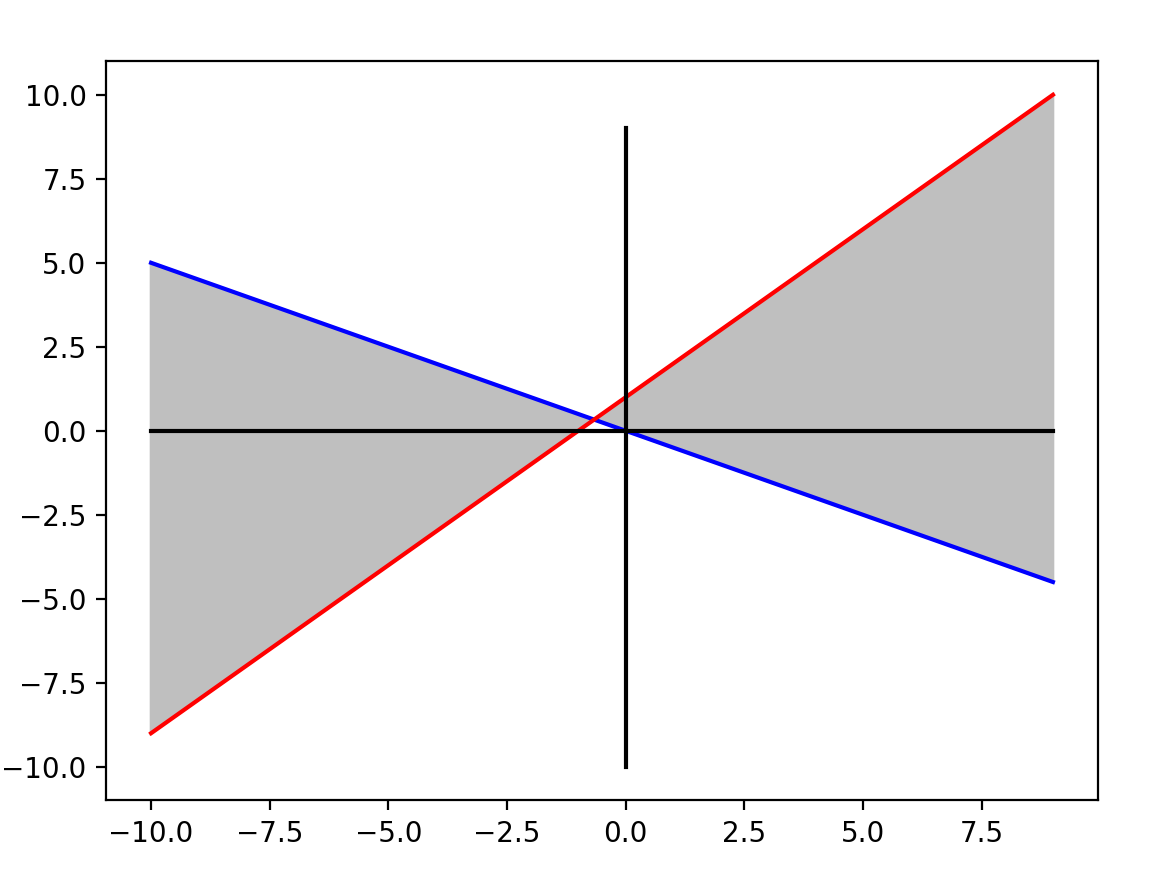
\includegraphics[scale=0.4]{EetF.png}
\end{center}
\begin{lstlisting}
import matplotlib.pyplot as plt
import numpy as np
plt.clf()
X=np.arange(-10,10,1)
Y=-X/2

plt.plot(X,Y,'b')
plt.plot(X,X+1,'R')
plt.plot(X,0*X,'black')
plt.plot(0*X,X,'black')

plt.fill([-2/3,9,9],[1/3,-4.5,10],color = '0.75')
plt.fill([-2/3,-10,-10],[1/3,5,-9],color = '0.75')
plt.show()
\end{lstlisting}
\item Ecrivons $P(x)$ sous la forme bien connue d'un polynôme du second degré : $P(x) = x^2 +x(y+1) -2y^2+2y$. On calcule son discriminant on obtient 
$$\Delta = (y+1)^2 -4 (-2y^2+2y) = 9y^2 - 6y +1= (3y-1)^2\geq 0$$
On obtient donc deux racines réelles (possiblement confondues) 
$$\frac{-y-1 \pm|3y-1|}{2} $$
$$-2y  \quadet  y-1$$
On peut donc écrire 
$$P(x) = (x+2y) (x-y+1)$$
Comme $y$ est arbitraire on obtient pour tout $(x,y) \in \R^2$, $$u(x,y) = (x+2y) (x-y+1)$$

Ainsi, $u(x,y) \geq 0$ si et seulement 

$$\left\{ 
\begin{array}{cc}
x+2y &\geq 0\\
x-y+1&\geq 0
\end{array}\right. 
\quadou 
\left\{ 
\begin{array}{cc}
x+2y &\leq 0\\
x-y+1&\leq 0
\end{array}\right.$$

$$\left\{ 
\begin{array}{cc}
y &\geq -\frac{x}{2}\\
y&\leq x-1
\end{array}\right. 
\quadou 
\left\{ 
\begin{array}{cc}
y &\leq -\frac{x}{2}\\
y&\geq x-1
\end{array}\right.$$
$$(x,y)\in E \quadou (x,y)\in F$$

Ainsi $$u(x,y)\geq 0 \equivaut (x,y) \in E\cup F$$



\end{enumerate}
\item \begin{enumerate}
\item Notons $g(t) = e^{\sqrt{t}}$. $g$ est définie est continue sur $\R^+$. Ainsi $f$ est bien définie pour tout $(x,y)\in \R^2$ tel que $u(x,y) \geq 0$ c'est-à-dire d'après la question précédente : $(x,y)\in E\cup F$. 
\item On calcule les dérivées partielles. Notons $G$  une primitive de $g$ sur $\R_+$ on  a 
$$f(x,y) = G(u(x,y)) -G(0).$$
Donc 
\begin{align*}
\frac{\partial f}{\partial x} (x,y) &= \frac{\partial u}{\partial x} (x,y) G'(u(x,y))\\
												&= (2x+y +1)e^{u(x,y)}
\end{align*}

et 

\begin{align*}
\frac{\partial f}{\partial y} (x,y) &= \frac{\partial u}{\partial y} (x,y) G'(u(x,y))\\
												&= (x-4y+2) e^{u(x,y)}
\end{align*}
D'où 
$$\nabla f  (x,y) = \left( \begin{array}{c}
 (2x+y +1)e^{u(x,y)}\\
  (x-4y+2) e^{u(x,y)}
\end{array}
\right)$$
\item \begin{align*}
\nabla f = \left( \begin{array}{c}
0\\
0
\end{array}
\right)
\quad &\equivaut\quad  \left( \begin{array}{c}
 (2x+y +1)e^{u(x,y)}\\
  (x-4y+2) e^{u(x,y)}
\end{array}\right) =\left( \begin{array}{c}
0\\
0
\end{array}
\right)\\
&\equivaut \left\{\begin{array}{cl}
2x+y +1&=0\\
x-4y+2&=0
\end{array}\right.\\
&\equivaut \left\{\begin{array}{cl}
x-4y&=-2\\
2x+y&=-1
\end{array}\right.\\
&\equivaut \left\{\begin{array}{ccl}
x&-4y&=-2\\
&9y&=3
\end{array}\right.\\
&\equivaut \left\{\begin{array}{ccl}
x&-4y&=-2\\
&y&=\frac{1}{3}
\end{array}\right.\\
&\equivaut \left\{\begin{array}{cl}
x&=-2+4\frac{1}{3} = \frac{-2}{3}\\
y&=\frac{1}{3}
\end{array}\right.\\
\end{align*}


\end{enumerate}
\item \begin{enumerate}
\item $u\left(\frac{-2}{3},\frac{1}{3}\right) =\left(\frac{-2}{3}\right)^2 +\left(\frac{-2}{3} \frac{1}{3}\right)  -\frac{2}{3}  -2 \left(\frac{1}{3}\right)^2 +2 \frac{1}{3} = 0$. Donc 
$$f\left(\frac{-2}{3},\frac{1}{3}\right) = 0$$
\item Pour tout $(x,y) \in D_f$, $u(x,y) \geq 0$ donc comme pour tout $t\geq 0, $  $e^{\sqrt{t}}>0$ on  a bien 
$$\int_0^{u(x,y)} e^{\sqrt{t}} dt \geq 0$$
et ainsi, $$u(x,y) \geq 0 =f\left(\frac{-2}{3},\frac{1}{3}\right)  $$
\item Tous les points 'au bord' de $E$ et $F$ satisfont $u(x,y)=0$ en effet si 
$x+2y = 0 $ ou $x-y+1=0$ on a bien $u(x,y) =0$ d'après la factorisation obtenue a la question 1b). 
Ces points n'ont pas un gradient nul alors que ce sont aussi des minima... Il n'y a pas de problème car dans le théorème disant "minima $\implique$ gradient nul" il faut que le point soit à \underline{intérieur} du domaine de définition. -
\end{enumerate}
\end{enumerate}

\end{correction}






%------------------------------------------------------------------------------------
%------------------------------------------------------------------------------------
%------------------------------------------------------------------------------------
%------------------------------------------------------------------------------------
%------------------------------------------------------------------------------------

\subsection{Intégrale de Gauss (D'après G2E 2019]}

\begin{exercice}[G2E 2019]
Dans cet exercice $\sigma$ désigne un réel strictement positif. \\

On considère les trois fonctions définies respectivement sur $\R$, $\R$ et $\R^*$ par :
$$
f_\sigma (x) = \left\{\begin{array}{lr}
0 & \text{si $x\leq 0,$}\\
\frac{x}{\sigma^2}e^{-\frac{x^2}{2\sigma^2}} &\text{si $x> 0$}
\end{array}\right. \quad g(x) =xe^{-x}, \quad h(x) = \frac{2}{ex}
$$
$\cC_\sigma$ désigne la courbe représentative de $f_\sigma$ et $\cH$ la courbe représentative de $h$
\begin{enumerate}
\item Soit $\ddp I_\sigma(t) = \int_0^t f_\sigma(x) dx$. Calculer $I_\sigma(t) $ pour tout $t\geq 0$ et en déduire la limite $\ddp \lim_{t\tv \infty} I_\sigma(t) $ \\
{\footnotesize L'année prochaine, on dira que $f_\sigma$ est une fonction de densité.}
\item $f_\sigma$ est-elle continue ? 
\item \begin{enumerate}
\item Démontrer que $g$ admet un maximum que l'on déterminera. 
\item En déduire que :
$$\forall x\in \R_+^*, \quad f_\sigma (x) \leq h(x).$$
\item Etudier le cas d'égalité dans l'inégalité précédente puis montrer que pour tout $\sigma \in \R^*_+$, les courbes $\cC_\sigma$ et $\cH$ ont une tangente commune dont on donnera une équation cartésienne. 
\end{enumerate}
\end{enumerate}

\end{exercice}

\begin{correction}
\begin{enumerate}
\item Considérons $F_\sigma$ définie par $F_\sigma(t) =-e^{-\frac{x^2}{2\sigma^2}}$ pour tout $x\geq 0$, $F_\sigma$ est dérivalbe sur $\R_+$ et on a pour $x\geq 0$, $F_\sigma'(x) = f_\sigma(x)$ ainsi
$$I_\sigma( t) =\left[ F_\sigma(x) \right]_0^t = F_\sigma(t) -F_\sigma(0)= e^{-\frac{t^2}{2\sigma^2}}+1.$$

Or $\lim_{t\tv \infty} e^{-\frac{t^2}{2\sigma^2}}=0$ donc 
$$\ddp \lim_{t\tv \infty} I_\sigma(t) =1.$$
\item $f_\sigma $ est continue sur $\R_- $ et $\R_+$ comme composée de fonctions usuelles. En $0$, 
$$\lim_{x\tv 0^+} f_\sigma(x)  = \lim_{x\tv 0^+} \frac{x}{\sigma^2}e^{-\frac{x^2}{2\sigma^2}}  =0$$ 
et 
$$\lim_{x\tv 0^-} f_\sigma(x)  = \lim_{x\tv 0^+} 0 =0$$ 
Ainsi $f_\sigma $ est continue en $0$ et finalement continue sur $\R$. 
\item 
\begin{enumerate}
\item $g$ est définie et dérivable sur $\R$ et on a pour tout $x\in \R$: 
$$g'(x) = e^{-x} -xe^{-x} = (1-x) e^{-x}$$
Ainsi $g$ est croissante sur $]-\infty, 0] $ et décroissante sur $[1,+\infty[$. 

$g$ atteint son maximum en $1$ et vaut $e^{-1}$. 
\item Pour tout $x> 0$ on   
\begin{align*}
f_\sigma(x)& = \frac{2}{x}  \frac{x^2}{2\sigma^2}e^{-\frac{x^2}{2\sigma^2}} \\
				&= \frac{2}{x}   g(\frac{x^2}{2\sigma^2})\\
				&\leq \frac{2}{x}   e^{-1} \quad \text{ d'après la question précédente} 
\end{align*}
 Ainsi $f_\sigma(x) \leq \frac{2}{ex} =h(x)$.  
\item L'égalité a lieu en $x_0\geq 0$ vérifiant $g(\frac{x_0^2}{2\sigma^2})=e^{-1} =g(1)$. On a vu à la question 3)a) que $e^{-1}$ était atteint uniquement en $1$ par $g$. On a  donc $\frac{x_0^2}{2\sigma^2} =1$. 
C'est-à-dire, comme $x_0\geq 0$, $$x_0=\sqrt{2}\sigma$$

On a bien $$f_\sigma (x_0) = \frac{\sqrt{2}}{\sigma} e^{-1} = \frac{2}{e \sqrt{2} \sigma} = h(x_0).$$

Ainsi $\cC_\sigma $ et $\cH$ ont bien un point en commun. Vérifions que les tangentes sont identiques en ce point. 

Tout d'abord remarquons ques les deux courbes admettent bien  des tangentes car sont des courbes représentatives de fonctions $\cC^1$. L'équation de la tangente à $\cC_\sigma$ en $x_0$ est donnée par 
$Y - f_\sigma(x_0) = f'_\sigma(x_0) (X-x_0)$
et on a $f'_\sigma(x_0) = \frac{1}{\sigma^2} e^{-\frac{x_0^2}{2\sigma^2}}  - \frac{x_0^2}{\sigma^4}e^{-\frac{x_0^2}{2\sigma^2}} $ ce qui donne en  simplifiant :
$$f'_\sigma(x_0) =  \frac{1}{\sigma^2} e^{-1} - \frac{2}{\sigma^2}e^{-1}= - \frac{1}{\sigma^2}e^{-1} $$

On obtient ainsi comme équation pour la tangente à $\cC_\sigma$ en $x_0$:
$$Y- \frac{\sqrt{2}}{e\sigma} = - \frac{1}{e\sigma^2} (X- \sqrt{2}\sigma)$$

Faisons de même avec la tangente à $\cH$ en $x_0$ et calculons $h'(x_0)$. 
On  a $h'(x_0) =\frac{-2}{ex_0^2}= \frac{-2}{e 2 \sigma^2} =- \frac{1}{e\sigma^2} =f'_\sigma(x_0) $
Ainsi les deux courbes admettent bien la même tangente en $x_0$ à savoir :

$$Y- \frac{\sqrt{2}}{e\sigma} = - \frac{1}{e\sigma^2} (X- \sqrt{2}\sigma)$$

 
\end{enumerate}
\end{enumerate}
\end{correction}













%------------------------------------------------------------------------------------
%------------------------------------------------------------------------------------
%------------------------------------------------------------------------------------
%------------------------------------------------------------------------------------
%------------------------------------------------------------------------------------






\subsection{Etude famille de fonction, intégrale, et somme (ECRICOME 2002)}

\begin{exercice}



On consid\`ere la famille de fonctions $(f_n)_{n\in\mathbb{N}^*}$ d\'efinies
sur $]-1,+\infty[$ par~: 
\begin{equation*}
f_n(x)=x^n\ln (1+x).
\end{equation*}


\paragraph{A- \'Etude des fonctions $f_n$.\\}




Soit $n\in \mathbb{N}^*$. On note $h_n$ la fonction d\'efinie sur $%
]-1,+\infty[$ par~: 
\begin{equation*}
h_n(x)=n\ln(1+x)+\frac{x}{1+x}.
\end{equation*}

\begin{enumerate}
\item \'{E}tudier le sens de variation des fonctions $h_{n}$.

\item Calculer $h_{n}(0)$, puis en d\'{e}duire le signe de $h_{n}$.

\item \'{E}tude du cas particulier $n=1$.

\begin{enumerate}
\item Apr\`{e}s avoir justifi\'{e} la d\'{e}rivabilit\'{e} de $f_{1}$ sur $%
]-1,+\infty [$, exprimer $f_{1}^{\prime }(x)$ en fonction de $h_{1}(x)$.

\item En d\'{e}duire les variations de la fonction $f_{1}$ sur $]-1,+\infty
[ $.
\end{enumerate}

\item Soit $n\in \mathbb{N}^{*}\setminus \{1\}$.

\begin{enumerate}
\item Justifier la d\'{e}rivabilit\'{e} de $f_{n}$ sur $]-1,+\infty [$ et
exprimer $f_{n}^{\prime }(x)$ en fonction de $h_{n}(x)$.

\item En d\'{e}duire les variations de $f_{n}$ sur $]-1,+\infty [$. (On
distinguera les cas $n$ pair et $n$ impair). On pr\'{e}cisera les limites
aux bornes sans \'{e}tudier les branches infinies.
\end{enumerate}
\end{enumerate}

\paragraph{B- \'Etude d'une suite.\\}

On consid\`ere la suite $\left(U_n\right)_{n\in\mathbb{N}^*}$ d\'efinie
par~: 
\begin{equation*}
U_n=\int_0^1f_n(x)\,dx.
\end{equation*}
\begin{enumerate}
\item Calcul de $U_1$.


\begin{enumerate}
\item Prouver l'existence de trois r\'{e}els $a$, $b$, $c$ tels que~: 
\begin{equation*}
\forall x\in [0,1],\quad \frac{x^{2}}{x+1}=ax+b+\frac{c}{x+1}.
\end{equation*}

\item En d\'{e}duire la valeur de l'int\'{e}grale~: 
\begin{equation*}
\int_{0}^{1}\frac{x^{2}}{x+1}\,dx.
\end{equation*}

\item Montrer que $\displaystyle U_{1}=\frac{1}{4}$.
\end{enumerate}

\item Convergence de la suite $\left(U_n\right)_{n\in\mathbb{N}^*}$\\

\begin{enumerate}
\item Montrer que la suite $\left( U_{n}\right) _{n\in \mathbb{N}^{*}}$ est
monotone.

\item Justifier la convergence de la suite $\left( U_{n}\right) _{n\in 
\mathbb{N}^{*}}$. (On ne demande pas sa limite.)

\item D\'{e}montrer que~: 
\begin{equation*}
\forall n\in \mathbb{N}^{*},\quad 0\leqslant U_{n}\leqslant \frac{\ln 2}{n+1}%
.
\end{equation*}

\item En d\'{e}duire la limite de la suite $\left( U_{n}\right) _{n\in 
\mathbb{N}^{*}}$.
\end{enumerate}


\item Calcul de $U_n$ pour $n\geqslant 2$


Pour $x\in [0,1]$ et $n\in \mathbb{N}^*\setminus \{1\}$, on pose~: 
\begin{equation*}
S_n(x)=1-x+x^2+\cdots+(-1)^nx^n=\sum_{k=0}^n(-1)^kx^k.
\end{equation*}

\begin{enumerate}
\item Montrer que~: 
\begin{equation*}
S_{n}(x)=\frac{1}{1+x}+\frac{(-1)^{n}x^{n+1}}{1+x}.
\end{equation*}

\item En d\'{e}duire que~: 
\begin{equation*}
\sum_{k=0}^{n}\frac{(-1)^{k}}{k+1}=\ln 2+(-1)^{n}\int_{0}^{1}\frac{x^{n+1}}{%
1+x}\,dx.
\end{equation*}

\item En utilisant une int\'{e}gration par parties dans le calcul de $U_{n}$%
, montrer que~: 
\begin{equation*}
U_{n}=\frac{\ln 2}{n+1}+\frac{(-1)^{n}}{n+1}\left[ \ln 2-\left( 1-\frac{1}{2}%
+\cdots +\frac{(-1)^{k}}{k+1}+\cdots +\frac{(-1)^{n}}{n+1}\right) \right] .
\end{equation*}
\end{enumerate}

\end{enumerate}

\end{exercice}





\begin{correction}
On consid\`ere la famille de fonctions $(f_n)_{n\in\mathbb{N}^*}$ d\'efinies
sur $]-1,+\infty[$ par~: 
\begin{equation*}
f_n(x)=x^n\ln (1+x).
\end{equation*}

\paragraph{A - \'Etude des fonctions $f_n$.}

Soit $n\in \mathbb{N}^{*}$. On note $h_{n}$ la fonction d\'{e}finie sur $%
]-1,+\infty [$ par~: 
\begin{equation*}
h_{n}(x)=n\ln (1+x)+\frac{x}{1+x}.
\end{equation*}

\begin{enumerate}
\item $h_{n}$ est d\'{e}rivable sur $]-1,+\infty [$ comme compos\'{e}e et
quotient de fonctions d\'{e}rivables et 
\begin{equation*}
h_{n}^{\prime }\left( x\right) =\frac{n}{1+x}+\frac{1+x-x}{\left( 1+x\right)
^{2}}=\frac{n+1+nx}{\left( 1+x\right) ^{2}}
\end{equation*}

Et comme $x>-1$ on a $nx>-n$ et $h_{n}^{\prime }\left( x\right) >0.$

Donc $h_{n}$ est strictement croissante sur $]-1,+\infty [$

\item On a : $h_{n}(0)=0$, et comme $h_{n}$ est strictement croissante, sur $%
]-1,0[$ on a :

\fbox{$h_{n}<0$ sur $]-1,0[$ et sur $]0,+\infty [$ on a $h_{n}>0$}

\item \'{E}tude du cas particulier $n=1$.

\begin{enumerate}
\item $f_{1}(x)=x\ln (1+x).$

La compos\'{e}e de $x\rightarrow 1+x$ d\'{e}rivable sur $]-1,+\infty [$ \`{a}
valeurs dans $]0,+\infty [$ o\`{u} $\ln $ est d\'{e}rivable.

Et $x\rightarrow x$ est d\'{e}rivable sur $\mathbb{R}$ donc $f_{n}$ est d%
\'{e}rivable sur $]-1,+\infty [$

\begin{equation*}
f_{1}^{\prime }(x)=\ln \left( 1+x\right) +\frac{x}{1+x}=h_{1}\left( x\right)
\end{equation*}

\item Donc $f_{1}$ est strictement d\'{e}croissante sur $]-1,0[$ et
strictement croissante sur $]0,+\infty [.$
\end{enumerate}

\item Soit $n\in \mathbb{N}^{*}\setminus \{1\}$.

\begin{enumerate}
\item Comme $n\in \mathbb{N}^{*},$ la fonction $x\rightarrow x^{n}$ est d%
\'{e}rivable sur $\mathbb{R}$ (la formule pour d\'{e}river serait diff\'{e}%
rente pour la puissance 0) donc (produit et somme ) $f_{n}$ est d\'{e}%
rivable sur $]-1,+\infty [$

\begin{eqnarray*}
f_{n}^{\prime }(x) &=&nx^{n-1}\ln (1+x)+\frac{x^{n}}{1+x}=x^{n-1}\left( n\ln
\left( 1+x\right) +\frac{x}{1+x}\right) \\
&=&x^{n-1}h_{n}\left( x\right)
\end{eqnarray*}

\item Donc si $n$ est pair, $n-1$ est impair donc

$n$ pair: 
\begin{tabular}{|c|ccccc|}
\hline
$x$ & -1 &  & 0 &  &  \\ \hline
$h_{n}\left( x\right) $ &  & $-$ & 0 & $+$ &  \\ \hline
$x^{n-1}$ &  & $-$ & 0 & $+$ &  \\ \hline
$f_{n}^{\prime }$ &  & $+$ & 0 & $+$ &  \\ \hline
&  &  &  & $\nearrow $ & $+\infty $ \\ 
$f_{n}\left( x\right) $ &  &  & 0 &  &  \\ 
& $-\infty $ & $\nearrow $ &  &  &  \\ \hline
\end{tabular}
$n$ impair : 
\begin{tabular}{|c|ccccc|}
\hline
$x$ & $-1$ &  & $0$ &  &  \\ \hline
$h_{n}\left( x\right) $ &  & $-$ & $0$ & $+$ &  \\ \hline
$x^{n-1}$ &  & $+$ & $0$ & $+$ &  \\ \hline
$f_{n}^{\prime }\left( x\right) $ &  & $-$ & $0$ & $+$ &  \\ \hline
$f_{n}\left( x\right) $ & $+\infty $ & $\searrow $ &  & $\nearrow $ & $%
+\infty $ \\ 
&  &  & $0$ &  &  \\ \hline
\end{tabular}

En -1, $x^{n}\rightarrow +1$ si $n$ est pair et $x^{n}\ln (1+x)\rightarrow
-\infty $ et $x^{n}\ln (1+x)\rightarrow +\infty $ si $n$ impair

En $+\infty :x^{n}\ln (1+x)\rightarrow +\infty $
\end{enumerate}
\end{enumerate}

\paragraph{B - \'{E}tude d'une suite.}

On consid\`ere la suite $\left(U_n\right)_{n\in\mathbb{N}^*}$ d\'efinie
par~: 
\begin{equation*}
U_n=\int_0^1f_n(x)\,dx.
\end{equation*}

\begin{enumerate}
\item Calcul de $U_1$.
\begin{enumerate}
\item Pour comparer, on met les deux expressions sous la m\^{e}me forme (m%
\^{e}me d\'{e}nominateur) en r\'{e}ordonnant par rapport aux puisances de $x$
: 
\begin{equation*}
ax+b+\frac{c}{x+1}=\frac{ax^{2}+\left( b+a\right) x+b+c}{x+1}
\end{equation*}

On a donc l'\'{e}galit\'{e} \textbf{si} $a=1$ et $b+a=0$ et $b+c=0$ soit $%
a=1 $, $b=-1$ et $c=1$

Une autre r\'{e}daction est de chercher ces coefficients au brouillon et de
constater que : 
\begin{equation*}
x-1+\frac{1}{x+1}=\frac{x^{2}}{x+1}
\end{equation*}%
et donc que $a=1$, $b=-1$ et $c=1$ conviennent

\item On peut alors d\'{e}terminer une primitive (la fonction int\'{e}gr\'{e}%
e est continue sur l'intervalle d'int\'{e}gration) et $x+1>0$ 
\begin{eqnarray*}
\int_{0}^{1}\frac{x^{2}}{x+1}\,dx &=&\int_{0}^{1}\left( x-1+\frac{1}{x+1}%
\right) dx=\left[ \frac{x^{2}}{2}-x+\ln \left( x+1\right) \right] _{x=0}^{1}
\\
&=&\ln \left( 2\right) -\frac{1}{2}.
\end{eqnarray*}

\item On a 
\begin{equation*}
U_{1}=\int_{0}^{1}f_{1}(x)\,dx=\int_{0}^{1}x\ln \left( 1+x\right) dx
\end{equation*}%
et en int\'{e}grant par partie (on d\'{e}rive le $\ln $ pour le faire dispara%
\^{\i}tre)

$u\left( x\right) =\ln \left( 1+x\right) ,$ $u$ de classe $C^{1}$ sur $\left[
0,1\right] $, $u^{\prime }\left( x\right) =\displaystyle
\frac{1}{1+x}$

$v^{\prime }\left( x\right) =x,$ $v^{\prime }$ est continue $v\left(
x\right) =x^{2}/2$%
\begin{eqnarray*}
U_{1} &=&\left[ \frac{x^{2}}{2}\ln \left( 1+x\right) \right]
_{0}^{1}-\int_{0}^{1}\frac{x^{2}}{2\left( 1+x\right) }dx=\frac{\ln \left(
2\right) }{2}-\frac{1}{2}\int_{0}^{1}\frac{x^{2}}{1+x}dx \\
&=&\frac{1}{4}
\end{eqnarray*}
\end{enumerate}

\item Convergence de la suite $\left( U_{n}\right) _{n\in \mathbb{N}%
^{*}}$.

\begin{enumerate}
\item Pour monter que la suite $\left( U_{n}\right) _{n\in \mathbb{N}^{*}}$
est monotone, il suffit de comparer $U_{n}$ et $U_{n+1}$.

Comme ce sont des int\'{e}grales, on compare leurs contenus sur $\left[ 0,1%
\right] $ :

$x^{n+1}-x^{n}=x^{n}\left( x-1\right) \le 0$ pour tout $x\in \left[ 0,1%
\right] $ et comme $\ln \left( 1+x\right) \ge 0$ sur $\left[ 0,1\right] $
(car $1+x\ge 1$) donc $x^{n+1}\ln \left( 1+x\right) \le x^{n}\ln \left(
1+x\right) $ et comme $0\le 1$ (ordre des bornes) on a alors 
\begin{equation*}
\int_{0}^{1}x^{n+1}\ln \left( 1+x\right) dx\le \int_{0}^{1}x^{n}\ln \left(
1+x\right) dx
\end{equation*}
et $U_{n+1}\le U_{n}.$

\textsl{Conclusion : }\fbox{la suite $U$ est d\'{e}croissante}

\item Toutes ces int\'{e}grales sont positive ou nulles car le contenu est
positif et les bornes sont en ordre croissant

Donc $U$ est d\'{e}croissante et minor\'{e}e par $0$donc convergente.

\item Pour encadrer l'int\'{e}grale, on encadre l\`{a} encore le contenu.
Pour obtenir $\frac{1}{n+1}$ on conserve le $x^{n}$ dans cet encadrement. On
se contente donc d'encadre le $\ln :$

Si $0\le x\le 1$ alors $1\le 1+x\le 2$ et comme $\ln $ est strictement
croissante sur $]0,+\infty [$ et que 1, $1+x$ et $2$ en sont \'{e}l\'{e}%
ments, $\ln \left( 1\right) \le \ln \left( 1+x\right) \le \ln \left(
2\right) .$

Comme $x^{n}\ge 0$ alors $0\le x^{n}\ln \left( 1+x\right) \le x^{n}\ln
\left( 2\right) $

Enfin comme $0\le 1:$%
\begin{equation*}
0\le \int_{0}^{1}x^{n}\ln \left( 1+x\right) dx\le \int_{0}^{1}x^{n}\ln
\left( 2\right) dx=\ln \left( 2\right) \left[ \frac{x^{n+1}}{n+1}\right]
_{0}^{1}=\frac{\ln \left( 2\right) }{n+1}
\end{equation*}
\textsl{Conclusion : }\fbox{$\forall n\in \mathbb{N}^{*}:\displaystyle
0\leqslant U_{n}\leqslant \frac{\ln 2}{n+1}$}

\item Et comme $\displaystyle
\frac{\ln 2}{n+1}\rightarrow 0,$ \fbox{par encadrement $U_{n}\underset{%
n\rightarrow +\infty }{\rightarrow }0$}
\end{enumerate}


\item Calcul de $U_n$ pour $n\geqslant 2$.

Pour $x\in [0,1]$ et $n\in \mathbb{N}^{*}\setminus \{1\}$, on pose~: 

\begin{equation*}
S_{n}(x)=1-x+x^{2}+\cdots +(-1)^{n}x^{n}=\sum_{k=0}^{n}(-1)^{k}x^{k}.
\end{equation*}
\begin{enumerate}
\item Comme $-x\ne 1$ on a : 
\begin{eqnarray*}
S_{n}(x) &=&\sum_{k=0}^{n}(-1)^{k}x^{k}=\sum_{k=0}^{n}(-x)^{k}=\frac{\left(
-x\right) ^{n+1}-1}{-x-1}. \\
&=&\frac{1}{1+x}-\frac{(-1)^{n+1}x^{n+1}}{1+x} \\
&=&\frac{1}{1+x}+\frac{(-1)^{n}x^{n+1}}{1+x}
\end{eqnarray*}

\item On a donc en int\'{e}grant l'\'{e}galit\'{e} pr\'{e}c\'{e}dente sur $%
\left[ 0,1\right] :$%
\begin{eqnarray*}
\int_{0}^{1}\sum_{k=0}^{n}(-1)^{k}x^{k}dx
&=&\sum_{k=0}^{n}(-1)^{k}\int_{0}^{1}x^{k}dx=\sum_{k=0}^{n}(-1)^{k}\left[ 
\frac{x^{k+1}}{k+1}\right] _{x=0}^{1} \\
&=&\sum_{k=0}^{n}\frac{(-1)^{k}}{k+1}
\end{eqnarray*}%
d'une part et d'autre part 
\begin{eqnarray*}
\int_{0}^{1}\sum_{k=0}^{n}(-1)^{k}x^{k}dx &=&\int_{0}^{1}\left( \frac{1}{1+x}%
+\frac{(-1)^{n}x^{n+1}}{1+x}\right) dx \\
&=&\int_{0}^{1}\frac{1}{1+x}dx+(-1)^{n}\int_{0}^{1}\frac{x^{n+1}}{1+x}dx \\
&=&\left[ \ln \left( 1+x\right) \right] _{0}^{1}+(-1)^{n}\int_{0}^{1}\frac{%
x^{n+1}}{1+x}dx \\
&=&\ln 2+(-1)^{n}\int_{0}^{1}\frac{x^{n+1}}{1+x}\,dx
\end{eqnarray*}%
et finalement 
\begin{equation*}
\sum_{k=0}^{n}\frac{(-1)^{k}}{k+1}=\ln 2+(-1)^{n}\int_{0}^{1}\frac{x^{n+1}}{%
1+x}\,dx.
\end{equation*}

\item On reconna\^{\i}t dans la formule propos\'{e}e $\displaystyle%
\sum_{k=0}^{n}\frac{(-1)^{k}}{k+1}$. On fait donc appara\^{\i}tre dans
l'expression de $U_{n}$ la quantit\'{e} $\displaystyle\int_{0}^{1}\frac{%
x^{n+1}}{1+x}\,dx:$

On a 
\begin{equation*}
U_{n}=\int_{0}^{1}x^{n}\ln \left( 1+x\right) dx
\end{equation*}
avec $u\left( x\right) =\ln \left( 1+x\right) $, $u$ est de classe $C^{1}$
sur $\left[ 0,1\right] $ et $u^{\prime }\left( x\right) =\displaystyle
\frac{1}{1+x}$

et avec $v^{\prime }\left( x\right) =x^{n}$ continue on a $v\left( x\right) =%
\displaystyle
\frac{x^{n+1}}{n+1}$ donc en int\'{e}grant par parties : 
\begin{eqnarray*}
U_{n} &=&\left[ \frac{x^{n+1}\ln \left( 1+x\right) }{n+1}\right]
_{x=0}^{1}-\int_{0}^{1}\frac{x^{n+1}}{\left( n+1\right) \left( 1+x\right) }dx
\\
&=&\frac{\ln 2}{n+1}-\frac{1}{n+1}\int_{0}^{1}\frac{x^{n+1}}{1+x}dx
\end{eqnarray*}
et de 
\begin{equation*}
\sum_{k=0}^{n}\frac{(-1)^{k}}{k+1}=\ln 2+(-1)^{n}\int_{0}^{1}\frac{x^{n+1}}{%
1+x}\,dx
\end{equation*}
on tire 
\begin{equation*}
\int_{0}^{1}\frac{x^{n+1}}{1+x}\,dx=(-1)^{n}\left[ \sum_{k=0}^{n}\frac{%
(-1)^{k}}{k+1}-\ln 2\right]
\end{equation*}

d'o\`{u} finalement 
\begin{equation*}
U_{n}=\frac{\ln 2}{n+1}+\frac{(-1)^{n}}{n+1}\left[ \ln 2-\left( 1-\frac{1}{2}%
+\cdots +\frac{(-1)^{k}}{k+1}+\cdots +\frac{(-1)^{n}}{n+1}\right) \right] .
\end{equation*}
\end{enumerate}

\end{enumerate}






%%%%%---
\subsection{Binome de Newton}


\begin{exercice}


\begin{enumerate}
\item Vérifier que la formule du binôme est vraie pour $n=0$, $n=1$, $n=2$ (et sur votre brouillon faite $n=3$).
On va prouver la formule par récurrence. On détaille les différentes étapes dans les prochaines questions: 
\item Montrer que $\forall (a,b)\in \bC^2,\,  \forall n \in \N, $:
$$\sum_{k=0}^n \binom{n}{k}a^{k+1} b^{n-k} = a^{n+1}+\sum_{k=1}^{n} \binom{n}{k-1}a^{k} b^{n-k+1}.$$


\item Montrer que $\forall (a,b)\in \bC^2,\,  \forall n \in \N, $
$$(a+b)\left( \sum_{k=0}^n \binom{n}{k}a^k b^{n-k}\right) = a^{n+1}+b^{n+1}+\sum_{k=1}^{n} \left( \binom{n}{k-1}+\binom{n}{k}\right)a^{k} b^{n-k+1}$$

\item En déduire que 
$$(a+b)\left( \sum_{k=0}^n \binom{n}{k}a^k b^{n-k}\right) = \sum_{k=0}^{n+1}  \binom{n+1}{k}a^{k} b^{n+1-k}$$

\item Conclure. 

Application : 
Soit $n,m\in \N^2$ 
\begin{enumerate}
\item Calculer $(1+x)^n(1+x)^m$  et $(1+x)^{n+m}$ à l'aide du binome de Newton. 
\item En déduire que pour tout $r\leq n+m$ on a : 
$$\sum_{j=0}^r  \binom{n}{j} \binom{m}{r-j}=\binom{n+m}{r}$$
%\item En déduire que pour tout $N\in \N^*$ et tout $n\in \intent{0,N}$ 
%$$\sum_{k=n}^N \binom{k}{n}=\binom{N+1}{n+1}$$
%(jouer avec les indices, changement de variables etc... ) 
\end{enumerate}


\end{enumerate}




\end{exercice}




\begin{correction}



\begin{enumerate}

\item Vérifier que la formule du binôme est vraie pour $n=0$, $n=1$, $n=2$ (et sur votre brouillon faite $n=3$).



\begin{enumerate}
\item $n=0$

On a 
$(a+b)^0 =1$ et 
$\sum_{k=0}^0 \binom{0}{k}a^k b^{0-k} = a^0b^0=1$

\item $n=1$

On a 
$(a+b)^1 =a+b$ et 
$\ddp \sum_{k=0}^1 \binom{1}{k}a^k b^{1-k} = \binom{1}{0}a^0 b^{1-0}+\binom{1}{1}a^1 b^{1-1}= a+b$


\item $n=2$

On a 
$(a+b)^2 =a^2+2ab+b^2$ et 
$\ddp \sum_{k=0}^2 \binom{2}{k}a^k b^{2-k} = \binom{2}{0}a^0 b^{2-0}+\binom{2}{1}a^1 b^{2-1}+\binom{2}{2}a^2 b^{2-2} =b^2+2ab+b^2$


\end{enumerate}
 









On va prouver la formule par récurrence. On détaille les différentes étapes dans les prochaines questions: 
\item Montrer que $\forall (a,b)\in \bC^2,\,  \forall n \in \N, $:
$$\sum_{k=0}^n \binom{n}{k}a^{k+1} b^{n-k} = a^{n+1}+\sum_{k=1}^{n} \binom{n}{k-1}a^{k} b^{n-k+1}.$$


\begin{align*}
\sum_{k=0}^n \binom{n}{k}a^{k+1} b^{n-k}  &= \sum_{k=0}^{n-1} \binom{n}{k}a^{k+1} b^{n-k}  + \binom{n}{n}a^{n+1} b^{n-n} \\
&= \sum_{k=0}^{n-1} \binom{n}{k}a^{k+1} b^{n-k}  + a^{n+1} 
\end{align*}
On fait le changement devariable $k+1=j$ sur la somme. On obtient 
$j\in \intent{1,n}$, donc 
$$\sum_{k=0}^{n-1} \binom{n}{k}a^{k+1} b^{n-k}  = \sum_{j=1}^{n} \binom{n}{j-1}a^{j} b^{n-j+1} $$
Comme $j$ est un indice muet, on peut le changer en $k$. On a donc la formule demandée.




\item Montrer que $\forall (a,b)\in \bC^2,\,  \forall n \in \N, $
$$(a+b)\left( \sum_{k=0}^n \binom{n}{k}a^k b^{n-k}\right) = a^{n+1}+b^{n+1}+\sum_{k=1}^{n} \left( \binom{n}{k-1}+\binom{n}{k}\right)a^{k} b^{n-k+1}$$



\begin{align*}
(a+b)\left( \sum_{k=0}^n \binom{n}{k}a^k b^{n-k}\right) &=a  \sum_{k=0}^n \binom{n}{k}a^k b^{n-k} +b\sum_{k=0}^n \binom{n}{k}a^k b^{n-k}\\
&= \sum_{k=0}^n \binom{n}{k}a^{k+1} b^{n-k} +\sum_{k=0}^n \binom{n}{k}a^k b^{n+1-k} 
\end{align*}
Maintenant on fait un changement de variable sur la première somme en posant $j =k+1$. On obtient : 
$$ \sum_{k=0}^n \binom{n}{k}a^{k+1} b^{n-k}= \sum_{j=1}^{n+1} \binom{n}{j-1}a^{j} b^{n-j+1}$$
On a donc, en se rappelant que $j$ est muet et donc remplacable par $k$
\begin{align*}
(a+b)\left( \sum_{k=0}^n \binom{n}{k}a^k b^{n-k}\right) &= \sum_{k=1}^{n+1} \binom{n}{k-1}a^{k} b^{n-k+1}+ \sum_{k=0}^{n} \binom{n}{k}a^{k} b^{n+1-k}
\end{align*}
On applique la relation de Chasles au  dernier terme de la première somme et au premier terme de la deuxième somme. On obtient : 

\begin{align*}
(a+b)\left( \sum_{k=0}^n \binom{n}{k}a^k b^{n-k}\right) &= \sum_{k=1}^{n} \binom{n}{k-1}a^{k} b^{n-k+1}+\binom{n}{n+1-1}a^{n+1} b^{n-(n+1)+1} \\& \hspace{2cm} +\sum_{k=1}^{n} \binom{n}{k}a^{k} b^{n+1-k} + \binom{n}{0}a^{0} b^{n+1-0} \\
&=  a^{n+1}+b^{n+1}+\sum_{k=1}^{n} \left( \binom{n}{k-1}+\binom{n}{k}\right)a^{k} b^{n-k+1}
\end{align*}




\item En déduire que 
$$(a+b)\left( \sum_{k=0}^n \binom{n}{k}a^k b^{n-k}\right) = \sum_{k=0}^{n+1}  \binom{n+1}{k}a^{k} b^{n+1-k}$$



On applique la relation obtenue dans la question 2 (relation de Pascal) à ce qu'on vient de trouver. 
$$\sum_{k=1}^{n} \left( \binom{n}{k-1}+\binom{n}{k}\right)a^{k} b^{n-k+1} = \sum_{k=1}^{n} \binom{n+1}{k}a^{k} b^{n-k+1}$$
Par ailleurs, 
$$a^{n+1} = \binom{n+1}{n+1}a^{n+1} b^{n-(n+1)+1}$$
et 
$$b^{n+1} = \binom{n+1}{0}a^{0} b^{n-0+1}$$
Ce sont donc les deux termes qui manquent à la somme de $0$ à $(n+1)$. ON a ainsi 
$$a^{n+1}+b^{n+1}+\sum_{k=1}^{n} \left( \binom{n}{k-1}+\binom{n}{k}\right)a^{k} b^{n-k+1} =\sum_{k=0}^{n+1}  \binom{n+1}{k}a^{k} b^{n+1-k}$$
Ce qui prouve le résultat grace à la question 5




\item Conclure. 



On fait une récurrence. On pose pour tout $n\in \N$:
$$\cP :' \forall a, b\in \bC, (a+b)^n =\sum_{k=0}^n \binom{n}{k}a^k b^{n-k}.$$
L'initialisation a été faite à la question 3.

L'hérédité correspond à la question 6. 

\paragraph{Application }

D'après le binome :
$$(1+x)^n(1+x)^m = \sum_{k=0}^n \binom{n}{k}x^k \times  \sum_{l=0}^m \binom{m}{l}x^l $$
Et par ailleurs 
$$(1+x)^{n+m} =  \sum_{j=0}^{n+m} \binom{n+m}{j}x^j$$

Comme $(1+x)^n(1+x)^m =(1+x)^{n+m}$ on peut identifier les  coefficients des deux polynomes. On obtient pour tout $r\in \intent{0,n+m}$
$$ \binom{n+m}{r} = \sum_{k,l, k+l=r}  \binom{n}{k} \binom{m}{l}$$
et 
$$ \sum_{k,l, k+l=r}  \binom{n}{k} \binom{m}{l} = \sum_{k=0}^n  \binom{n}{k} \binom{m}{r-k}$$




\end{enumerate}










\end{correction}

























%------------------------------------------------------------------------------------
%------------------------------------------------------------------------------------
%------------------------------------------------------------------------------------
%------------------------------------------------------------------------------------
%------------------------------------------------------------------------------------






\subsection{inéquation à paramétre - Une bien l'autre pas finie}

\begin{exercice}
On considère l'inéquation $(E_a)$ de paramètre $a\in \R$ suivante  :
$$ \frac{2x+a}{x-4a}  \leq \frac{x}{x-2a} \quad (E_a)$$

\begin{enumerate}
\item Donner l'ensemble des solutions pour $a=0$\\

Pour la suite on supppose que $a\neq 0$.
\item Donner le domaine de définition de $(E_a)$ en fonction de $a$. 
\item Résoudre pour $a>0$ l'inéquation : $(x-4a)(x-2a)\geq 0$.
\item Résoudre pour $a>0$ l'inéquation : $x^2+ax-2a^2\geq 0$.
\item En déduire pour $a>0$ les solutions de $(E_a)$. 
\item Faire de même avec $a<0$. 
\end{enumerate}
\end{exercice}
%%%----
\begin{correction}
\begin{enumerate}
\item Pour $a=0$, l'équation devient $(E_0)  : \frac{2x}{x} \leq \frac{x}{x}$ 
C'est-à-dire $$2\leq 1$$. 
\conclusion{ $(E_0)$ n'admet pas de solution.}
\item L'équation est bien définie pour tout $x-4a \neq 0$ et $x -2a\neq 0$. 
\conclusion{ Le domaine de définition de $(E_a)$ est $\R\setminus\{ 2a,4a\}$}
\item Remarquons que pour $a>0$, $4a>2a$, les solutions de $(x-4a)(x-2a)\geq0$ sont donc 
\conclusion{ $S_1 = ]-\infty , 2a[ \cup ]4a, +\infty[$}
\item Regardons le discriminant de $x^2 +ax-2a^2 $. On obtient 
$\Delta = a^2 +4a^2 = 9a^2$.
Ainsi il y a deux racines réelles distinctes (rappelons que $a\neq 0$ ) 
$$r_1 = \frac{-a +\sqrt{9a^2}}{2} = a \quadet r_2  = \frac{-a -\sqrt{9a^2}}{2} = -2a$$
On  a donc $$x^2 +ax-2a^2  = (x-a)(x+2a)$$
(Remarquons par ailleurs que cette égalité est aussi vraie pour $a<0$, ceci nous sera utile pour la question 6) 
Les solutions  de $x^2 +ax-2a^2 \geq 0 $ sont donc 
\conclusion{ $] -\infty, -2a[\cup ]a, +\infty[$}
\item 
\begin{align*}
(E_a) \equivaut & \frac{2x+a}{x-4a} -\frac{x}{x-2a} \leq 0\\
		\equivaut & \frac{(2x+a)(x-2a) -(x-4a)x}{(x-4a)(x-2a)}\leq 0\\		
		\equivaut & \frac{(2-1)x^2+(-4a+a+4a)x -2a^2)}{(x-4a)(x-2a)}\leq 0\\		
		\equivaut & \frac{x^2+ax -2a^2}{(x-4a)(x-2a)}\leq 0	\\			
		\equivaut & \frac{x^2+ax -2a^2}{(x-4a)(x-2a)}\leq 0	
\end{align*}
  \begin{tikzpicture}

     \tkzTabInit[lgt=4,espcl=2]
       {$x$ / 1 , $x^2+ax -2a^2$ / 1, $(x-4a)(x-2a)$ / 1  ,  $\ddp \frac{x^2+ax -2a^2}{(x-4a)(x-2a)}$ /1.5 }
       {$-\infty$, $-2a$, $a$, $2a$, $4a$,$+\infty$}
       \tkzTabLine
       { ,+ , z,- , z ,+ , d, +, d, + , }
       \tkzTabLine
		{ ,+ , , +,  ,+ , d, -, d, + , }
       \tkzTabLine
		{ ,+ ,z , -, z ,+ , d, -, d, + , }
  \end{tikzpicture}
  
 Ainsi les solutions sont 
 \conclusion{ $S_a =[-2a,a] \cup ]2a,4a[$}
 
 \item Pour $a<0$, la seule chose qui change est l'ordre des  valeurs $-2a,a,2a,4a$. On a dans ce cas : $4a<2a <a<-2a$ et donc le tableau de signes suivant : 
 
 
  \begin{tikzpicture}

     \tkzTabInit[lgt=4,espcl=2]
       {$x$ / 1 , $x^2+ax -2a^2$ / 1, $(x-4a)(x-2a)$ / 1  ,  $\ddp \frac{x^2+ax -2a^2}{(x-4a)(x-2a)}$ /1.5 }
       {$-\infty$, $4a$, $2a$, $a$, $-2a$,$+\infty$}
       \tkzTabLine
       { ,+ , d,+ , d ,+ , z, -, z, + , }
       \tkzTabLine
		{ ,+ , d, -, d ,+ , , +, , + , }
       \tkzTabLine
		{ ,+ ,d , -, d ,+ , z, -, z, + , }
  \end{tikzpicture} 
  Ainsi les solutions pour $a<0$ sont 
 \conclusion{ $S_a =]4a,2a[ \cup [a,-2a]$}
 
\end{enumerate}
\end{correction}


\begin{exercice}
On considère l'équation $(E_a)$ de paramètre $a\in \R$ suivante  :

$$ \sqrt{x+a^2} =\frac{a^2}{x-a} \quad (E_a)$$

On note $\cS_a$ l'ensemble des solutions de $(E_a)$ 
\begin{enumerate}

\item 
\begin{enumerate}
\item Determiner $\cC$ l'ensemble des solutions de l'inéquation d'inconnue $a\in \R$, $-a^2\leq a$.
\item Déterminer en fonction de $a\in \R$  l'ensemble de définition $\cD_a$ de l'équation $(E_a)$. 
\item Résoudre l'équation $(E_0)$.
\item A quelle condition sur $a\in \R$, le nombre $0$ est il solution de $(E_a)$ ? (En d'autres termes, déterminer l'ensemble des $a\in \R$ tel que $0\in \cS_a$) 
\end{enumerate}
% A partir de maintenant et jusqu'à la fin, on supposera que $a>0$
\item Résoudre pour $x\in \cD_a$ et en fonction de $a\in \R$ l'inéquation : $$\frac{a^2}{x-a} < 0$$
(On distinguera les cas $a\in \cC$ et $a\notin \cC$)
\item En déduire que $\cS_a \subset ]a,+\infty[$. 
\item Montrer que pour tout $x>a$, 
$$(E_a) \equivaut x^2 +(a^2-2a)x +(a^2-2a^3)=0$$
\item Soit $\Delta_a$ le discriminant du polynôme $ x^2 +(a^2-2a)x +(a^2-2a^3)$. 
Montrer que $$\Delta_a =a^3 (a+4)$$
\item En déduire une expression simple de l'ensemble $P =\{ a >0 \, |\, \Delta_a \geq 0\}$

\item Résoudre finalement $(E_a) $ en fonction de $a$ (On suppose toujours $a>0$)


\end{enumerate}

\end{exercice}

\begin{correction}
\begin{enumerate}
\item \begin{enumerate}
\item $-a^2\leq a \equivaut a^2+a\geq 0 \equivaut a(a+1) \geq 0$
L'ensemble des solutions est dont 
\conclusion{$\cC = ]-\infty, -1[ \cup ]0,+\infty[$}

\item L'équation est bien défiinie pour $x$ vérifiant  :
$$x+a^2\geq 0 \quadet x-a\neq 0$$
C'est à dire $x\geq -a^2 $ et $x\neq a$. 

On obtient deux cas 
\begin{itemize}
\item Si $a\in \cC$ :  $$D_a= ]-a^2,a[\cup ]a, +\infty[$$
\item Si $a\notin \cC:$  $$D_a= ]-a^2,+\infty[$$
\end{itemize}  

\item L'équation $(E_0) \equivaut \sqrt{x} =0$, dont la seule solution sur $\R$ est $x=0$. Mais l'ensemble de définition est $]0,+\infty[$, donc 
\conclusion{ $(E_0)$ n'admet pas de solution. }
\item $0\in \cS_a\equivaut \sqrt{a^2} = \frac{a^2}{-a} \equivaut |a | =-a$.
Ainsi \conclusion{ $0 \in \cS_a$ pour tout $a \in \R_-^*$} 


\end{enumerate}
\item Comme $a^2>0$: $$\frac{a^2}{x-a}<0 \equivaut x-a<0 \equivaut x<a$$
L'ensemble des solutions est donc 
\conclusion{ $]-\infty, a[$}

\item Comme la fonction racine est positive, pour que $x$ soit une solution de $(E_a)$ il faut que $\frac{a^2}{x-a}\geq 0$. Ainsi l'ensemble des solutions des inclus dans le complémentaire des solutions de l'inéquation précédente : $\cS_a \subset [a,+\infty[$. Mais $a\notin D_a$ donc 
\conclusion{ $\cS_a\subset]a, +\infty[$}

\item Pour $x>a$, les deux membres sont positifs, on peut donc élever au carré l'équation. On obtient :
%\begin{align*}
%(E_a)\equivaut &x+a^2 =\left(\frac{a^2}{x-a}\right)^2\\
%\equivaut & x+a^2 - \frac{a^4}{(x-a)^2}=0\\
%\equivaut &(x+a^2)(x-a)^2  -a^4=0 \quad \text{ car (x-a)^2\neq 0} \\
%\equivaut & (x+a^2)(x^2-2ax+a^2)-a^4=0\\
%\equivaut & (x^3 +(a^2-2a)x^2 +(a^2 -2a^3)x +a^4) -a^4=0\\
%\equivaut & x (x^2 + (a^2-2a) x + (a^2-2a^3)) =0\\
%\equivaut & x^2 + (a^2-2a) x + (a^2-2a^3)  =0\quad \text{ car x\neq 0} 
%\end{align*}

On obtient bien pour $x>a$ :
\conclusion{ $(E_a) \equivaut  x^2 + (a^2-2a) x + (a^2-2a^3)  =0$}

\item
\begin{align*}
\Delta_a &= (a^2-2a)^2 - 4(a^2-2a^3) \\
				&= a^2(a-2)^2 - 4a^2(1-2a) \\
				&=a^2 (a^2-4a+4 -4(1-2a))\\
				&=a^2 (a^2 +4a)\\
				&=a^3(a+4)
\end{align*}

\item P(

\end{enumerate}
\end{correction}
